\UseRawInputEncoding
\documentclass[a4paper,oneside,12pt]{book}
\usepackage[utf8]{inputenc}
\usepackage[T1]{fontenc}
\usepackage{lmodern}

\usepackage[style=phys,biblabel=brackets]{biblatex} 
\addbibresource{bibliography.bib}

\usepackage{minted}
\usepackage[minted]{tcolorbox}
\newtcblisting{mylisting}{listing only,listing engine=minted, minted language=matlab,colback=gray!20}

\usepackage{amsbsy}
\usepackage{amssymb}
\usepackage{amsmath}
\usepackage{graphicx}
\usepackage{multirow}
\usepackage{mathrsfs}
\usepackage{color}
\usepackage{enumitem}
\usepackage{epsfig}
\usepackage{caption}
\usepackage{subcaption}
\usepackage[strict]{changepage}
\usepackage{csquotes}
\usepackage{lipsum}
\usepackage{tikz}
\usetikzlibrary{shapes}
\usetikzlibrary{arrows, arrows.meta}
\usepackage{ifthen}
\usepackage{relsize}
\usepackage{physics}
\usepackage{textcomp}
\usepackage{placeins}
\usepackage{algorithm}
\usepackage[noend]{algpseudocode}
\usepackage{xpatch}
\xpatchcmd{\algorithmic}{\itemsep\z@}{\itemsep=2ex plus2pt}{}{}
\usepackage{dcolumn}

\DeclareCiteCommand{\fullcite}
  {\usebibmacro{prenote}}
  {\usedriver
     {\defcounter{minnames}{6}%
      \defcounter{maxnames}{6}}
     {\thefield{entrytype}}.}
  {\multicitedelim}
  {\usebibmacro{postnote}}  
  
% Page Margins - Strath Requirement
\usepackage[
left=4cm,
right=2.5cm,
top=2cm,
bottom=4cm,
includehead,
includefoot,
headheight=28pt
]{geometry}

% Page Headers
\usepackage{fancyhdr}
\usepackage{setspace}
\setstretch{1.5}
\setlength{\parindent}{0pt}

\usepackage{titling}
\usepackage{tocloft}
\usepackage[hidelinks]{hyperref}

\raggedbottom

% Custom commands

\newcommand\blfootnote[1]{%
  \begingroup
  \renewcommand\thefootnote{}\footnote{#1}%
  \addtocounter{footnote}{-1}%
  \endgroup
}

\newcommand*{\Heff}{\hat{H}_\text{eff}}
\newcommand*{\expectation}[1]{\langle#1\rangle}

\begin{document}
	
    \frontmatter

    \pagestyle{empty}
\begin{titlepage}
   \begin{center}
       \vspace*{0.5cm}

       \textbf{\LARGE Measurement-Induced Phase Transitions and the Interplay between Coherent and Dissipative Dynamics}

       \vspace{1.5cm}
            
       
\includegraphics[width=0.4\textwidth]{Logos/strath_fullcolour.png}
       
       \LARGE University of Strathclyde 
            
       \textit{\Large Department of Physics and SUPA}\\
       
       \vspace{1.0cm}

       \Large Tom Bintener \\
       \Large{September 2023}

       \vspace{1cm}
       
       \textit{\Large A thesis submitted in partial fulfilment \\ 
		of the requirements for the degree of \\
		Doctor of Philosophy} \\

        \vspace{1cm}
            
   \end{center}
\end{titlepage}
\cleardoublepage 


	\pagestyle{empty}
\vspace*{0.2\textheight}

\begin{center}
    \vspace{0.9cm}

    \begin{flushleft}
	
	This thesis is the result of the author's original research. It has been composed by the author and has not been previously submitted for examination which has led to the award of a degree. \\[5pt]
	%
	The copyright of this thesis belongs to the author under the terms of the United Kingdom Copyright Acts as qualified by University of Strathclyde Regulation 3.50. Due acknowledgement must always be made of the use of any material contained in, or derived from, this thesis. \\[5pt]
	%
	\vspace{1cm}
	\end{flushleft}
 
	\begin{flushleft}
		Signed: \\
		\vspace{0.3cm}
		Date: 	
	\end{flushleft}
    
\end{center}

% Declaration
\topskip0pt
\vspace*{\fill}
\noindent

\cleardoublepage

	

	\pagestyle{empty}
\vspace*{0.2\textheight}

{\itshape Fascinating Story. Any Chance You're Nearing The End?\bigbreak}

\hfill - Geralt of Rivia


    \newgeometry{
left=4cm,
right=2.5cm,
top=2cm,
bottom=4cm
}

\chapter*{Preface}
\addcontentsline{toc}{section}{Preface}

In May 2019, I started working on the project that is the focus of chapter~\ref{chap:MIPT_bosons}. Towards the final stages of the project in 2020, we became aware of a paper \cite{fuji2020}, which investigated a very similar model, which led to the decision not to publish our manuscript. Regardless of this decision, I have contributed to new insight into the physics of measurement-induced phase transitions in continuous-time systems. I explored and analyzed different models and presented transitions manifesting in the entanglement entropy in individual trajectories, presented in chapter~\ref{chap:MIPT_bosons}.

Moreover, I have expanded our understanding of why these transitions are so difficult to measure directly in experiments. Although some quantities, like the entanglement entropy, visualize the transition quite clearly, the exact location of the transition is quite difficult to pinpoint. This difficulty is also discussed in chapter~\ref{chap:MIPT_bosons}, and the presented analysis provides new insight into the difficulties that were not discussed in the existing literature. Furthermore, I proved why, in a homodyne detection scheme, you cannot use the measurement outcomes to reconstruct nonlinear functions that witness the transition. The reason why this is the case is subtle, and it is the focus of chapter~\ref{chap:MIPT_continuous_measurement}.

Lastly, I have explored the consequences of competition between dissipative and coherent processes for many-body dynamics at short to medium times. I have investigated the signatures of the transitions we can observe at short times in models that undergo phase transitions in the long time limit of non-linear functions of the density operator. In addition, I have explored how this short-time competition might be investigated. This topic is the focus of chapter~\ref{chap:short_time_dynamics}. \\

Overall, I have generated both new theoretical understanding, of interest to theorists in this particularly topical area, and also experimental proposes, especially for exploring competition between coherent and dissipative processes in short-time dynamics. \\

\textbf{Publications during the Ph.D.}
\begin{enumerate}
    \item \fullcite{bintener2024}

    This paper is the topic of chapter~\ref{chap:short_time_dynamics}. To be submitted to Physical Review A, 2024.
\end{enumerate}

\cleardoublepage

    \newgeometry{
left=4cm,
right=2.5cm,
top=2cm,
bottom=4cm}
\chapter*{Acknowledgements}
\addcontentsline{toc}{section}{Acknowledgements}

After spending almost a third of my life in Glasgow, pursuing both my undergraduate and postgraduate studies at Strathclyde, I am deeply grateful to everyone who has made this journey unforgettable and supported me every step of the way. \\

First and foremost, I would like to express my heartfelt thanks to my supervisor, Andrew Daley, for granting me the opportunity to undertake this PhD under his exceptional guidance and unwavering support. Under his mentorship, I have acquired a wealth of knowledge in physics and honed numerous skills that have prepared me for my professional career. \\

I am also profoundly grateful to my fellow PhD students and post-docs in our group: Callum, François, Gerard, Johannes, Liam, Rosaria, and Sridevi. Special thanks go to Jorge for being a true friend and providing immense help throughout my PhD. I would also like to acknowledge Jacopo, Stuart, and Tomohiro, who were always ready to offer their assistance whenever needed. \\

Next, I extend my gratitude to my friends: Ahmed, Amine, and Athina, for their companionship since our first days in Glasgow; Eduardo, for sharing countless dark beverages and making music together; Iro, for her friendship and for showing me the beauty of Athens; the Shuttlecock Destroyers—Jack, Johan, and Jorge—for the fun and camaraderie on the badminton court; and finally Nicole, for being an incredible flatmate and the greatest prankster I've had the pleasure to meet. \\

I am especially thankful to my girlfriend, Maria, for her unwavering support, particularly during the challenging process of writing this thesis. Her motivation and encouragement have been invaluable. \\

Finally, I would like to thank my family for their support throughout this journey. Their encouragement has always driven me to strive for better. Merci.

\vspace{1cm}
\hspace*{\fill} \textit{Bintener Tom, 01.09.2023}

\cleardoublepage
\restoregeometry
    
	\newgeometry{
left=4cm,
right=2.5cm,
top=2cm,
bottom=4cm
}
\chapter*{Abstract}
\addcontentsline{toc}{section}{Abstract}

Measurement-induced phase transitions arise from the interplay of coherent quantum dynamics and local measurements. For example, coherent dynamics can generate entanglement and long-ranged correlations, while local measurements destroy them. By tuning the strength of the measurements, the system undergoes a phase transition at the level of individual stochastic measurement trajectories. It is only witnessed by non-linear functions in the density operator, and due to the stochastic nature of the measurement outcomes, the average density operator masks the transition. 

In this thesis, we explore how this type of transition arises in bosonic and fermionic models that are subject to dephasing or measurement and consider ways to detect the transition in experiments. We first give an overview of the transition and describe the difficulties in identifying the exact location of the transition and finding experimental protocols to detect them. We then show that in a homodyne detection setup, it is impossible to reconstruct the nonlinear correlation function that witnesses the transition, using only the linear information from homodyne currents, and we discuss the difficulties that arise when considering the experimental detection of this transition. We finally show that features of the competition between coherent and dissipative dynamics are already present at short times during the system evolution. We also present a protocol that displays the characteristic behavior of the transition, starting from an infinite temperature state. 

In all projects, we employ a range of numerical techniques, such as Monte-Carlo wavefunction methods, which allow us to simulate the open quantum systems dynamics and enable us to explore the presented models.

\cleardoublepage
\restoregeometry


	
    \tableofcontents 
    
    \mainmatter

    \chapter{Introduction}
\thispagestyle{empty}
\label{chap:intro}
    
    \pagestyle{fancy}
    \renewcommand{\chaptermark}[1]{ \markboth{#1}{} }
    \renewcommand{\sectionmark}[1]{ \markright{#1}{} }
    \fancyhead{}
    \fancyhead[R]{\leftmark}
    \fancyhead[R]{\rightmark}
    \fancyfoot{}
    \renewcommand{\footrulewidth}{0.4pt}
    \fancyfoot[R]{\thepage}

In recent years, the competition between coherent and dissipative dynamics in many-body quantum systems has been studied, which has led to the emergence of novel types of dynamical phase transitions known as measurement-induced phase transitions (MIPTs) \cite{li2018,li2019,chen2020,skinner2019,bao2020,jian2020,zabalo2020,zhang2020,gullans2020,bentsen2021a}.  In chapter~~\ref{chap:MIPT_bosons}-\ref{chap:short_time_dynamics}, we study this competition between coherent and dissipative dynamics in continuous time models and analyze some scenarios in which MIPTs arise. We begin by providing a brief overview and introducing this novel transition type.

\section{Overview}

The field of quantum many-body physics explores emergent properties of ensembles of many quantum particles, such as atoms, electrons, or photons, interacting with each other according to the laws of quantum mechanics. These systems can give rise to new exciting physics, such as the behavior of ultra-cold atomic gases in optical lattices \cite{bloch2012} or the emergence of novel phases of matter in condensed matter systems \cite{bernevig2013}.

The interplay of quantum mechanics of how particles interact in quantum many-body systems leads to novel and often unexpected phenomena, such as quantum phase-transitions, high-temperature superconductivity \cite{leggett2006}, thermalization \cite{srednicki1994} and novel states of matter such as superfluidity \cite{schmitt2015} or Bose-Einstein condensation \cite{georgescu2020}, which have both fundamental significance and potential technological applications.

Furthermore, quantum many-body physics plays a vital role in investigating fundamental problems in fields such as quantum information theory. For example, exploring the entanglement structure of quantum many-body states gives valuable insight into the potential use in quantum information processing tasks \cite{luecke2014, schmied2016, luo2017}. Quantum entanglement is an interesting property of quantum many-body states, as it characterizes the non-classical correlations in the system. When two or more quantum systems are entangled, their properties, such as spin or polarization, become correlated so that the state of one system instantaneously affects the state of the others, regardless of the distance between them. Such non-local correlations challenge classical intuition and form the basis of various quantum technologies, including quantum cryptography, quantum teleportation, and quantum computing. A quantum many-body system is said to be entangled when the quantum states of individual particles that make up the system cannot be described independently of the state as a whole \cite{nielsen2000}. In other words, if the wave function of the system cannot be written as the product of the wave function of two subsystems that make up the whole system, then these subsystems are entangled. 

\begin{figure}[ht]
    \centering
    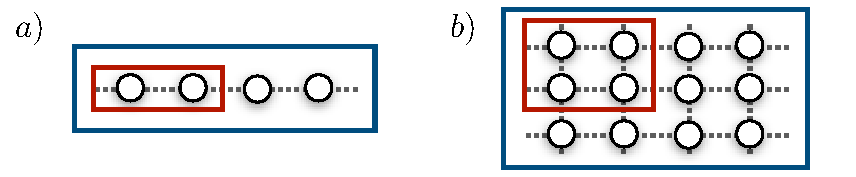
\includegraphics[width=\textwidth]{Chapters/Plots/Chapter1/Chapter0_Fig2.pdf}
    \caption{Schematic representation of a quantum many-body system consisting of particles on a lattice in a) 1D and b) 2D. The blue boundary denotes the total quantum system, and the red boundary denotes a subsystem of the total quantum system.} 
    \label{fig:Chapter0_Fig2}
\end{figure}

Mathematically, we formulate this as $\ket{\psi_{AB}} \neq \ket{\psi_A} \ket{\psi_B}$, where $\ket{\psi_{AB}}$ denotes the wave function of the whole system, and $\ket{\psi_A}, \ket{\psi_B}$ denote the wave functions of the subsystems A and B, respectively. In contrast, if a quantum system is not entangled, it is possible to express it as the product of subsystems, $\ket{\psi}_{AB} = \ket{\psi}_A \ket{\psi}_B$, and we can fully describe either subsystem independently of the system as a whole. For this reason, such states are also known as separable states. Quantum entanglement has a range of useful applications, such as in quantum cryptography \cite{pirandola2020}, where entangled states can be used for quantum key distribution protocols (see, e.g., \cite{ekert1991}) that ensure that nobody intercepted the communication. Entanglement provides a sensitive probe, such as for quantum thermalization \cite{deutsch1991,rigol2008,dalessio2016}, information scrambling \cite{srednicki1994,trail2008,bentsen2019}, or the characterization of quantum phases \cite{calabrese2004}.

In quantum information processing, entanglement is connected to quantum resource theories, defined by some operations classes. Choosing, for instance, local operations and classical communication as the set of operations that can be used, only separable (non-entangled) states can be created under this class \cite{horodecki2013}. Since entangled states cannot be created under this class of operations, they become a resource as they cannot be created for 'free'. Given entangled states, however, performing tasks that would otherwise not be possible via the allowed operations becomes possible~\cite{nielsen,horodecki2009,horodecki2013}. Entanglement measures provide useful ways to quantify how much entanglement (or, in other words, quantum correlations) there is (are) in a system \cite{plenio2006}, and one important measure is the von Neumann entropy ($S_{VN}$), which we will use throughout this thesis. The von Neumann entropy is an entanglement measure that quantifies the amount of entanglement present in a pure system. Let us consider again a quantum state $\hat{\rho}_{AB} = \ket{\psi_{AB}}\bra{\psi_{AB}}$, where A and B denote two subsystems that make up the whole system. To quantify the amount of entanglement present between the two subsystems, $A$ and $B$, we can use the von Neumann entropy of the reduced system $S_{VN}(\hat{\rho}_A) = S_{VN}(\Tr_B(\hat{\rho}_{AB}))$, where $\Tr_B$ denotes the partial trace over the subsystem $B$. 

Computational simulation of quantum many-body systems dynamics is challenging as the Hilbert space in which quantum states live grows exponentially with the number of particles in the system. In a system that consists of $n$ 2-level systems, $2^n$ complex coefficients are needed to describe the state fully. Consequently, for simulations, $2^n$ complex numbers must be stored in a computer, which quickly becomes impossible for many particles. In quantum computing \cite{forcer2002, nandhini2022}; however, a superposition of $2^n$ states can be represented using $n$ 2-level systems, which can lead to exponential speed-ups for certain problems and is also known as quantum parallelism. Moreover, entanglement plays a vital role in quantum computing, as it has been shown that to achieve exponential speed-up over classical computation, multipartite entanglement (i.e., entanglement between more than just two subsystems) is needed in the system \cite{jozsa2003}. One of the most well-known algorithms benefitting from this exponential speed-up is Shor's algorithm for factoring numbers into their prime factors\cite{shor1997}.

\begin{figure}[ht]
    \centering
    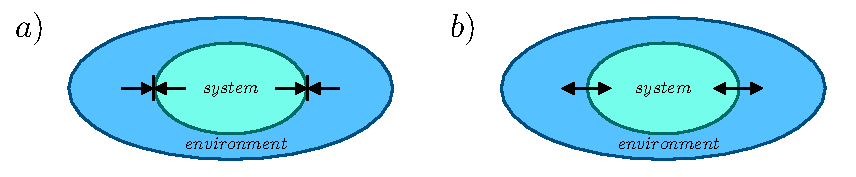
\includegraphics[width=\textwidth]{Chapters/Plots/Chapter1/Chapter0_Fig4.pdf}
    \caption{Schematic representations of a) a closed and b) an open quantum system. The closed quantum system does not interact with the environment nor exchange matter or energy, as indicated by the arrows blocked by the solid black lines. In contrast, an open quantum system does interact with its environment. It is a more realistic representation, as it is essentially impossible to guarantee that no energy or particles leave the system of interest.}
    \label{fig:Chapter0_Fig4}
\end{figure}

The closed system behavior of a many-body quantum system is prescribed by the Schr\"{o}dinger equation, leading to the description of the unitary time evolution of the density operator. Moreover, in isolated systems that thermalize, the entanglement entropy of a subsystem is extensive \cite{nandkishore2015}, corresponding to linear growth of entanglement entropy with subsystem size in $1D$, also known as \textit{volume-law} scaling of the entanglement entropy. 

In reality, however, no quantum system is ever truly isolated, leading to dissipative processes that prevent the system from evolving unitarily. Such dissipative processes can occur either as a result of measurements being voluntarily performed by an observer or simply due to the coupling to the environment, resulting in loss of information. More specifically, local measurements (such as projective measurements) tend to decrease the amount of entanglement present in the system by projecting the wave function on a given site to be in a definite state, effectively disentangling it from the rest of the system. One question that arises is whether or not the volume-law scaling of the entropy in thermalizing systems survives when local measurements are performed, as they reduce the total amount of entanglement present in the system. 

\begin{figure}[ht]
    \centering
    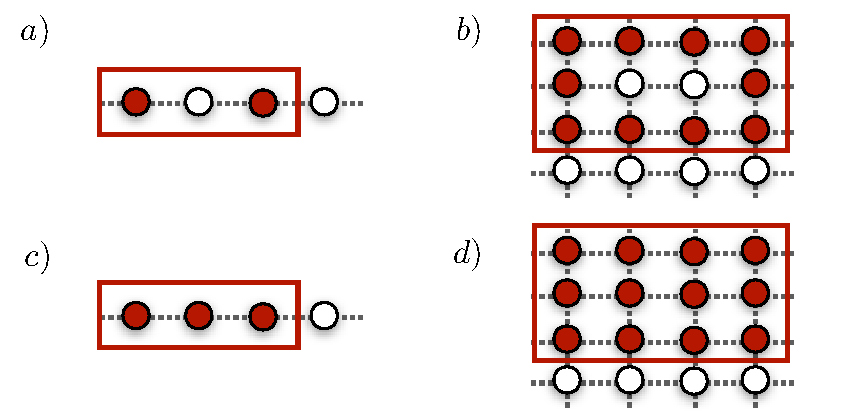
\includegraphics[width=\textwidth]{Chapters/Plots/Chapter1/Chapter0_Fig3.pdf}
    \caption{Schematic representation of the area of the boundary in a) $1D$ and b) $2D$, and the volume of the boundary in c) $1D$ and d) $2D$. In $1D$, the area will remain constant, no matter how much the subsystem grows, as only one (or two if one considers periodic boundary conditions) cut(s) are needed to divide the system into two subsystems. Therefore, if the entropy is constant with subsystem size, we call this area-law, as we will see in later chapters. On the other hand, the volume consists of all the particles contained within the subsystem, which grows linearly as the subsystem grows. We, therefore, speak of volume-law entanglement when the entropy grows linearly with the subsystem size. Similarly, in $2D$, the area grows linearly with subsystem size while the volume grows quadratically, and analogous to the $1D$ case, one speaks of area and volume-law scaling of the entropy when the entropy of the subsystem scales either linearly or quadratically with the boundary.}
    \label{fig:Chapter0_Fig3}
\end{figure}

As we have discussed, having access to quantum states that withstand disentangling dynamics is particularly useful for quantum computers and simulators, where entangled states serve as an important resource. Therefore, it is important to understand the effect of measurements on unitary dynamics, as it allows us to characterize the entanglement properties of states in novel dynamical quantum phases that may be employed in quantum computers.

The competition between coherent and local dissipative dynamics has led to the notion of measurement-induced phase transitions (MIPTs), which were first discovered in random circuits. The competition arises because coherent dynamics can build up the total amount of entanglement in the system, while local dissipative dynamics tend to decrease it. We will now provide a brief overview of MIPTs in the context of random circuits before we discuss them in continuous time models.

\subsection{MIPTs in Random Circuits}

 MIPTs have been explored in recent years in random circuit models \cite{li2018,li2019,skinner2019,bao2020,jian2020,zabalo2020,zhang2020,lang2020, moghaddam2023,martin-vazquez2023} where it has been shown that continuous phase transitions arise as a result of the competition between entangling unitary dynamics and disentangling local measurements. These transitions are characterized by the qualitative change in the wave function undergoing a measurement trajectory, making it crucial to track measurement outcomes.

\begin{figure}[ht]
    \centering
    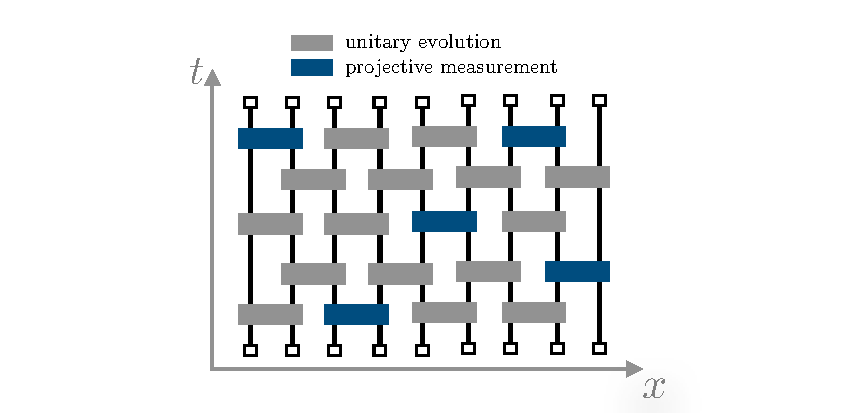
\includegraphics[width=\textwidth]{Chapters/Plots/Chapter1/Chapter0_Fig5.pdf}
    \caption{Schematic representations of hybrid circuit model. The unitary gates (gray) are applied pairwise on neighboring qubits. The projective measurements (blue) are applied randomly in time (t) and space (x) before applying the unitary gates.}
    \label{fig:Chapter0_Fig5}
\end{figure}

Refs.~\cite{li2018,li2019,skinner2019} present a phase transition in a hybrid circuit model (Fig.~\ref{fig:Chapter0_Fig5}), where an initial non-entangled product state is time-evolved by applying random unitary gates drawn from various distributions. The unitary evolution is interrupted by performing projective measurements randomly in time and space with a probability $p$ per unitary gate. No projective measurements occur for $p \to 0$, while for $p \to 1$, projective measurements are applied before each unitary gate. The entanglement grows over time with this model, and the steady-state exhibits volume-law scaling of the entanglement entropy for small measurement probabilities, indicated by linear growth of the entropy with the subsystem size. Then, at a critical measurement probability, it undergoes a phase transition into a ``quantum Zeno'' regime \cite{itano1990}. In this regime, measurements occur frequently, suppressing the entanglement growth, resulting in the area-law scaling of the entropy, where the entropy is constant and independent of the subsystem size.

As mentioned before, these transitions are characterized by qualitative changes in the measurement trajectories, and it is important to note that at the level of the density operator, this transition is masked. As the measurement outcomes are random, after a long time evolution, each local measurement outcome is obtained roughly equally. This has the consequence that upon averaging over all measurement outcomes, any state in the Hilbert space is equally likely corresponding to an infinite temperature state. For any nonzero measurement probability, given enough time, the infinite temperature state is reached, and therefore, the transition is not accessible. 

Other types of transitions have also been explored in random circuits, such as purification transitions \cite{gullans2020,bentsen2021a} where an initially mixed state is time evolved while subjected to continuous measurement. As the measurements destroy quantum correlations between subsystems, the entropy also decreases. Above a critical measurement strength, the average entropy decays to zero independent of the system size, implying that as a result of the measurements, we know what the state of the system is. Below the critical measurement strength, the entanglement is not entirely destroyed, and the time to purify the system grows exponentially with the system size.  

Not only are these transitions of fundamental interest, but they can also be related to the generation of error correction codes in quantum channels \cite{choi2020,gullans2021,fan2021,li2021}, where they arise during the unitary time evolution and protect the volume-law phase against disentangling projective measurements. Furthermore, there has been progress in probing these entanglement transitions \cite{gullans2020a,noel2022}. In Ref.~\cite{gullans2020a}, the authors propose the entropy of a reference qubit entangled with a system of interest as an order parameter for a MIPT. Below the critical measurement strength, the entropy of the reference qubit can stay nonzero while it decays to zero above the critical measurement strength. In Ref.~\cite{noel2022}, the authors probe the transition using the probe proposed in \cite{gullans2020a} on a trapped-ion quantum computer and find experimental evidence of the two phases by measuring the entropy of the reference qubit.

\subsection{MIPTs in Continuous Time Models}

\begin{figure}[ht]
    \centering
    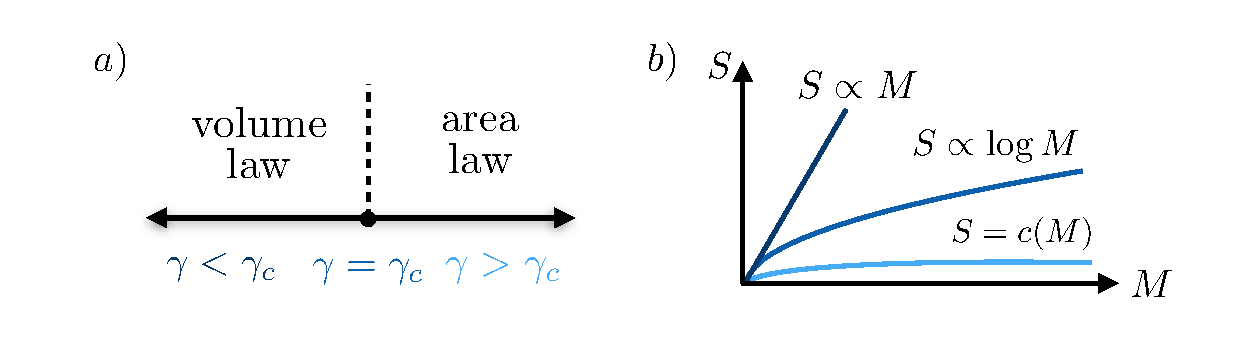
\includegraphics[width=\textwidth]{Chapters/Plots/Chapter1/Chapter0_Fig1.pdf}
    \caption{a) Schematic representation of a phase diagram in a non-integrable model that exhibits a measurement-induced phase transition at a critical measurement strength $\gamma_c$ from volume law scaling of the entropy to area-law scaling. b) Schematic representation of the characteristic behavior of the entropy; close to criticality, the entropy scales logarithmically with the subsystem size $M$, the volume-law phase is characterized by linear growth of the entropy, and in the area-law phase, the entropy grows minimally and remains constant.}
    \label{fig:Chapter0_Fig1}
\end{figure}

As we have just discussed, random circuits have been explored in depth in recent years \cite{fisher2022}, and a natural question is whether the same entanglement transition can be seen in continuous time models. This type of transition has also been investigated in spin chains and bosonic systems \cite{fuji2020,tang2020,biella2021,doggen2022, botzung2021, muller2022}. Refs.~\cite{fuji2020,tang2020,doggen2022} investigate a bosonic system, where they break the integrability of the model to witness a stable volume-law scaling phase. They find an entanglement transition where a qualitative change from volume-law scaling to area-law scaling of the entropy occurs. The characteristic behavior of this transition is schematically represented in Fig.~\ref{fig:Chapter0_Fig1}. Integrable models tend to possess many symmetries \cite{retore2022}, which means they are exactly solvable. Non-integrable models, on the other hand, are not exactly solvable, and it has been shown that they exhibit volume-law scaling of the entanglement entropy \cite{nakagawa2018}. Interestingly, as we will see, MIPTs can arise in both integrable and non-integrable models. 

A chain of non-interacting free fermions has been shown to have no volume-law phase for arbitrarily small measurement strengths \cite{cao2019} and an area-law phase that is present for any nonzero measurement rates. It was later shown \cite{alberton2021} that the model exhibits a phase transition where the entanglement entropy scales logarithmically with the subsystem size for small but nonzero measurement rates. At a critical rate of the measurements, the system undergoes a phase transition beyond which the entropy exhibits area-law scaling. In later chapters, we will also analyze these transitions and discuss the difficulties of accurately identifying them. Some schemes have been proposed to observe these transitions, using pre-selection \cite{buchhold2022}, where the stationary state of the model can be altered by steering the system towards a specific state that does not destroy the underlying properties that result in the transition.

In Ref.~\cite{doggen2022}, a transition was predicted in the Ising model, where the transverse magnetization is monitored. Similar to other systems, a transition in the quantitative behavior of the wave function occurs; however, instead of using the entanglement entropy, they consider the overlap between the trajectory steady-state and the localized quantum Zeno product state, which characterizes at which point the dissipative dynamics take over.

\subsection{Challenges}

As previously mentioned, the MIPTs are masked at the density operator level for random circuits. In continuous models, where dissipation in the form of dephasing occurs, the steady-state obtained through averaging over all possible measurement outcomes is the trivial infinite temperature state, independent of measurement strength. Similarly, by considering the master equation, which describes such a system, it also always reaches the infinite temperature state, so we cannot directly use the master equation to find the signatures of MIPTs in steady-states of continuous time models. Instead, we need to consider non-linear quantities, such as the entanglement entropy at the quantum trajectory level, to access these transitions. These quantities need to be evaluated at the trajectory level before computing the average over all trajectories as linear quantities, which would again correspond to the expectation value in the infinite temperature state. Another challenge to overcome is to extract these non-linear quantities from individual trajectories, as generally, multiple measurements on a single trajectory are required to access these quantities. Suppose measurements are made deterministically in time and repeatable for specific measurement outcomes in these systems. In that case, it is theoretically possible to extract quantities like the entanglement entropy of subsystems by repeating trajectories and performing measurements with the interference of copies \cite{islam2015, daley2012} or random unitaries \cite{elben2018, brydges2019}. 

However, the measurement results are typically not reproducible - and more commonly, they are not even known when the dissipation comes from natural coupling to the environment or random noise. In this case, performing more than one measurement on a single trajectory is impossible, and techniques for extracting the entanglement entropy cannot be used. Here, we consider what can be realized in such realistic and also small, finite-sized systems corresponding, e.g., to current 1D experiments in quantum gas microscopes \cite{bakr2009, sherson2010, gross2021}. The random entangling gates are replaced by unitary dynamics of interacting dipolar bosons on a 1D lattice \cite{patscheider2020}. In contrast, the random measurements are replaced by local dephasing, which can be readily realized for ultracold gases through noise or light scattering~\cite{luschen2017,pichler2010,sarkar2014,poletti2013}. By looking at the trajectories corresponding physically to dephasing events at particular positions and locations, we can find a similar change in behavior moving between area- and volume-law entanglement growth as we change the dephasing rate. Investigating the steady-state properties of quantum trajectories will be the main focus of chapters \ref{chap:MIPT_bosons} and \ref{chap:MIPT_continuous_measurement}.

These difficulties are somewhat reduced when we relax the focus on steady-state dynamics and also consider short- or intermediate-time dynamics. In this case, at long times, the steady-state remains the infinite temperature state, and the master equation cannot be used to detect signatures of the MIPTs. Interestingly, however, by investigating how the system in question reaches the infinite temperature state, signatures of the transitions are present in both non-linear and linear quantities in the density operator. Obviously, for non-linear quantities, the order in which we compute the average and quantity still matters. However, this is not the case for linear quantities (such as the local densities), and here, in principle, the master equation approach can also be employed to investigate the system and gain information on the transition signatures. However, it is essential to note that the transition itself cannot be detected this way, as this is only possible in the steady-state where the master equation approach does not work. The signatures that are present at early and intermediate times are the focus of chapter \ref{chap:short_time_dynamics}. Although it is, in principle, possible to use the master equation approach in some cases that we just discussed, we continue to use the trajectory approach, as we are not only interested in the evolution of the average values but also in the statistics when many trajectories are simulated as we gain additional information from the statistics and how the quantities are distributed.

\section{Thesis Outline}

In chapter~\ref{chap:intro}, we have introduced the main background ideas that have inspired the work presented in this thesis. We introduced measurement-induced phase transitions in the context of random circuits where they were first studied and in continuous time models. \\

In chapter~\ref{chap:phase_sec}, we will discuss classical and quantum phase transitions to provide a brief overview of this topic. We will consider a simple example to introduce the main concepts that we need to study the phase transitions presented in the following chapters. \\

Chapter~\ref{chap:tech_sec} focuses on the main tools and methods used to simulate open quantum systems numerically. We outline the derivation of the Lindblad master equation, which describes the time evolution of an open quantum system subject to dissipative processes. We then introduce the Monte Carlo wave function method to simulate the master equation more efficiently. Finally, we discuss homodyne detection and quantum state diffusion, which provide another unraveling of the master equation, also allowing us to simulate the master equation numerically.  \\

In chapter~\ref{chap:MIPT_bosons}, we study a chain of interacting hardcore bosons subject to dephasing. We present a measurement-induced phase transition that arises from the competition between coherent and dissipative processes manifesting in the entanglement entropy. We use the main ideas introduced in chapter~\ref{chap:intro}-\ref{chap:phase_sec} to characterize the phase transition and highlight the limitations we encounter in the model. We also provide a detailed discussion on the scaling collapses for the system sizes we can simulate and turn to free fermions to allow for the simulation of larger systems. Finally, we explicitly break the $U(1)$ symmetry conserved in the model and investigate whether we still see this phase transition. \\

In chapter~\ref{chap:MIPT_continuous_measurement}, we attempt to find a way to witness the quantum phase transition experimentally, which is no easy task as the quantities witnessing the transition need to be non-linear in the density operator. We show for a class of correlation functions how this rules out the possibility of measuring them experimentally. \\

In chapter~\ref{chap:short_time_dynamics}, we relax the constraints of focusing exclusively on steady-state properties by considering non-linear as well as linear quantities at early times. We show that signatures of the competition between coherent and dissipative dynamics can be resolved even at early times. This allows us to propose an experimental protocol that can probe the competition between coherent and dissipative dynamics in the model. \\

In chapter\ref{chap:conclusion}, we conclude the thesis and summarize what we have learned by undertaking the projects discussed in chapter~\ref{chap:MIPT_bosons}-\ref{chap:short_time_dynamics}. 

	
	\chapter{Phase Transitions}
\thispagestyle{empty}
\label{chap:phase_sec}

We have already introduced the ideas of measurement-induced phase transitions, and in this chapter, we provide a general overview of phase transitions. We briefly discuss classical phase transitions, and then, with the help of a simple model, we introduce the main tools, such as correlation functions, that we use in the coming chapters to analyze the MIPTs in a few different models.

\section{Classical Phase Transitions}

Classical phase transitions (CPTs) surround us in our everyday lives, and everyone has, at some point, experienced them firsthand. As we enjoy a drink on a hot summer day, we see the ice cubes melting and cooling down the glass. At atmospheric pressure, water freezes at $0^\circ C$ and boils at $100^\circ C$, and at these points, it undergoes a phase transition. Although everyone is familiar with these processes happening in everyday life, the physics behind them is quite interesting. Phase transitions are defined via discontinuities in the free energy derivatives with respect to thermal variables such as pressure or temperature. If we consider water, the quantity that shows drastic changes is the density. The density is proportional to the inverse of the volume, which in turn is related to the first derivative of the free energy with respect to pressure. An ice cube will float in a glass of water, so we know its density is lower than liquid water. If we heat ice, it will absorb heat, and its temperature will continuously rise until it has reached $0^\circ C$. At this point, the energy put into the system will not further heat the ice but will melt it. The energy needed to convert ice to liquid water at the critical temperature entirely is also known as \textit{latent heat}. Once all the ice has melted, it will continue to increase in temperature as more heat is added to the system until it reaches $100^\circ C$, where it will stop rising in temperature until the latent heat has wholly converted the liquid water into water vapor. At each of these points, while the temperature remains constant, the density changes, such that at atmospheric pressure and at $0^\circ C$ ($100^\circ C$), ice and liquid water (liquid water and vapor) have two densities. This discontinuity in the density defines these transition points, and as the discontinuity occurs in the first derivative of the free energy, these phase transitions involving latent heat are known as \textit{first-order} phase transitions. 

However, there are many more phases than just the ones we are familiar with in our everyday life. An iron magnet is ferromagnetic and produces a stable magnetic field; however, if heated to high enough temperatures, it undergoes a phase transition and becomes paramagnetic. To witness the transition, we typically choose an order parameter that exhibits distinct behavior in the two phases. For this example, magnetization is a useful order parameter. In the ferromagnetic phase, the spins are all aligned in the same direction, giving rise to non-zero total net magnetization. As the temperature increases, thermal fluctuations will start to destroy the ferromagnetic ordering, leading to a decrease in net magnetization. The magnetization will be zero at a critical temperature, and we enter the paramagnetic phase. Now, the spins randomly fluctuate around and have no preferred direction, and therefore, the net magnetization is zero at temperatures greater than the critical temperature. This is an example of a \textit{second-order phase transition}, or alternatively known as a \textit{continuous phase transition} due to the magnetization continuously decreasing to zero as the temperature increases and crosses the critical temperature. Another way of looking at this is by considering the symmetry present in the system. If we think about the direction rather than the magnitude of the magnetization vector, we see that this also allows us to characterize the phase transition as well. As mentioned before, the spins have no preferred direction at high temperatures, which is why the magnetization is zero. As no particular direction is preferred, we can describe this system as being rotationally invariant. Below the critical temperature, however, all spins are aligned in some direction, which means this rotational invariance of the system is no longer present, which is also known as spontaneous symmetry breaking.

More generally, symmetries are defined in symmetry groups, such as rotations or translations. For example, a two-dimensional rotation around an angle $\theta = 2 \pi/n$ generates the $\mathbb{Z}_n$ group. This describes the various symmetries that one encounters in nature, and the spontaneous breaking of symmetries is associated with phase transitions \cite{sachdev2011}. Furthermore, close to the critical point, the behavior of the order parameter can be investigated, and a critical exponent can be extracted. This exponent describes how the order parameter or a correlation function decays at criticality. Such critical exponents have been used to define universality classes, where the idea is that one can classify different types of transitions by their critical exponents \cite{odor2004}. Models belonging to a universality class do not necessarily exhibit the same behavior away from criticality; however, their behavior becomes increasingly similar close to it. 

\section{Quantum Phase Transitions}

After introducing some examples and features of phase transitions in general, let us now consider quantum phase transitions (QPTs)~\cite{sachdev2011, vojta2002, vojta2003,  heyl2018}. QPTs are phase transitions that occur in a quantum system at zero temperature. Hence, they do not occur as the result of tuning a thermal parameter but rather some other system parameter, such as a coupling term in the Hamiltonian. Therefore, thermal fluctuations cannot be the reason for quantum phase transitions to occur; instead, they are caused by quantum fluctuations. 

An example of a quantum phase transition can be seen in the transverse Ising model, where the Hamiltonian is defined by,
\begin{equation}
    \label{eq:transIsing}
    \hat{H} = -J \sum\limits_i \hat{\sigma}^z_i \hat{\sigma}^z_{i+1} - h \sum_i \hat{\sigma}^x_i,
\end{equation}

where $J$ is the interaction strength, $h$ the coupling strength of an external magnetic field in the $x$-direction, and $\hat{\sigma}^z_i, \hat{\sigma}^x_i$ are the Pauli matrices on site $i$. The transverse Ising model is the quantum equivalent of the classical Ising model. It is one of the simplest models exhibiting a quantum phase transition, allowing us to highlight the main concepts we use in later chapters to present measurement-induced phase transitions. In this section, we will focus on the quantum phase transition in $1D$. However, dynamical quantum phase transitions in this model in $2D$ have also been explored in recent years \cite{halimeh2017, hashizume2022}. Dynamical quantum phase transitions can occur when an initial state is prepared under a Hamiltonian with some initial control parameter, such as $h$ in Eq.~\ref{eq:transIsing} and then exploring the dynamics resulting from quenching the control parameter. Let us now explore some common tools used to highlight and explore quantum phase transitions in the $1D$ transverse Ising model.

The Transverse Ising Hamiltonian is invariant under flipping all spins in the $z$-direction. It is easy to verify that $\comm{\hat{H}}{\hat{P}} = 0$, where $\hat{P}$  is the spin-flip operator $\hat{P}  = \prod_i \hat{\sigma}^x_i$. A spin flip corresponds to a rotation about an angle $\theta = \pi$, which we mentioned earlier generates the $\mathbb{Z}_2$ group. As the Hamiltonian is invariant under this transformation, we say that it possesses a $\mathbb{Z}_2$ symmetry group. For the following analysis, we will consider $J = 1$ to define units of energy. 

A quantum system at absolute zero will be in its ground state, and without an external magnetic field ($h = 0$), the Hamiltonian exhibits two degenerate ground states, the two ferromagnetic states with all spins pointing either up ($\ket{\uparrow}$) or down ($\ket{\downarrow}$) in the $z$-direction. In reality, however, there is always a small external magnetic field that breaks this degeneracy, and the system favors one of these two states. Neither of these two states is invariant under the spin-flip operator, 
\begin{align}
\begin{split}
    \hat{P}  \ket{\uparrow} & = \ket{\downarrow} \\
    \hat{P}  \ket{\downarrow} & = \ket{\uparrow},
\end{split}
\end{align}
where $\ket{\uparrow}, \ket{\downarrow}$ are the two eigenstates of $\sigma_z$,
\begin{align}
\begin{split}
    \hat{\sigma}^z \ket{\uparrow} & = \ket{\uparrow} \\
    \hat{\sigma}^z \ket{\downarrow} & = - \ket{\downarrow}.
\end{split}
\end{align}

Then, as the coupling to the magnetic field $h$ is increased, there is a competition for the spins to all align (or anti-align) along the $z$ or the $x$ direction, which results in the order of the ferromagnetic ground state being destroyed. There are two degenerate ground states in the two limits $h = 0$ and $h \to \infty$. When choosing one ground state in a numerical simulation, one needs to select an eigenvector with the smallest eigenvalue. Due to the degeneracy, the chosen ground state will depend on the programming language or algorithm that is used in the simulation, leading to inconsistent results if we use the magnetization. For consistency, we therefore define an order parameter $P_{FM}$ given by the probability of finding the ground state in either one of the two ferromagnetic states, 
\begin{equation}
    P_{FM} = |\braket{\uparrow}{\psi}|^2 + |\braket{\downarrow}{\psi}|^2, 
\end{equation}
where $\ket{\psi}$ is the ground state that is found by the simulation. 

In Fig.~\ref{fig:Chapter1_Fig1}a), we see that for small $h$, the order parameter is $1$, indicating the ferromagnetic ordering of the ground state. As $h$ is increased, the ferromagnetic ordering of the ground state is destroyed, and the system undergoes a quantum phase transition at $h = 1$. In the limit $h \to \infty$ the ground state will point along the $x$-direction, where each spin will be in the superposition $\ket{\xrightarrow{}} = \frac{1}{\sqrt{2}}(\ket{\uparrow}+\ket{\downarrow})$. This state clearly is invariant under the spin-flip operator, $\hat{P}  \ket{\xrightarrow{}} = \ket{\xrightarrow{}}$. This phenomenon is known as spontaneous symmetry breaking. This phase transition is an example of a continuous phase transition, where the order parameter continuously changes with $h$, but the $\mathbb{Z}_2$-symmetry is broken. 

\begin{figure}[ht]
    \centering
    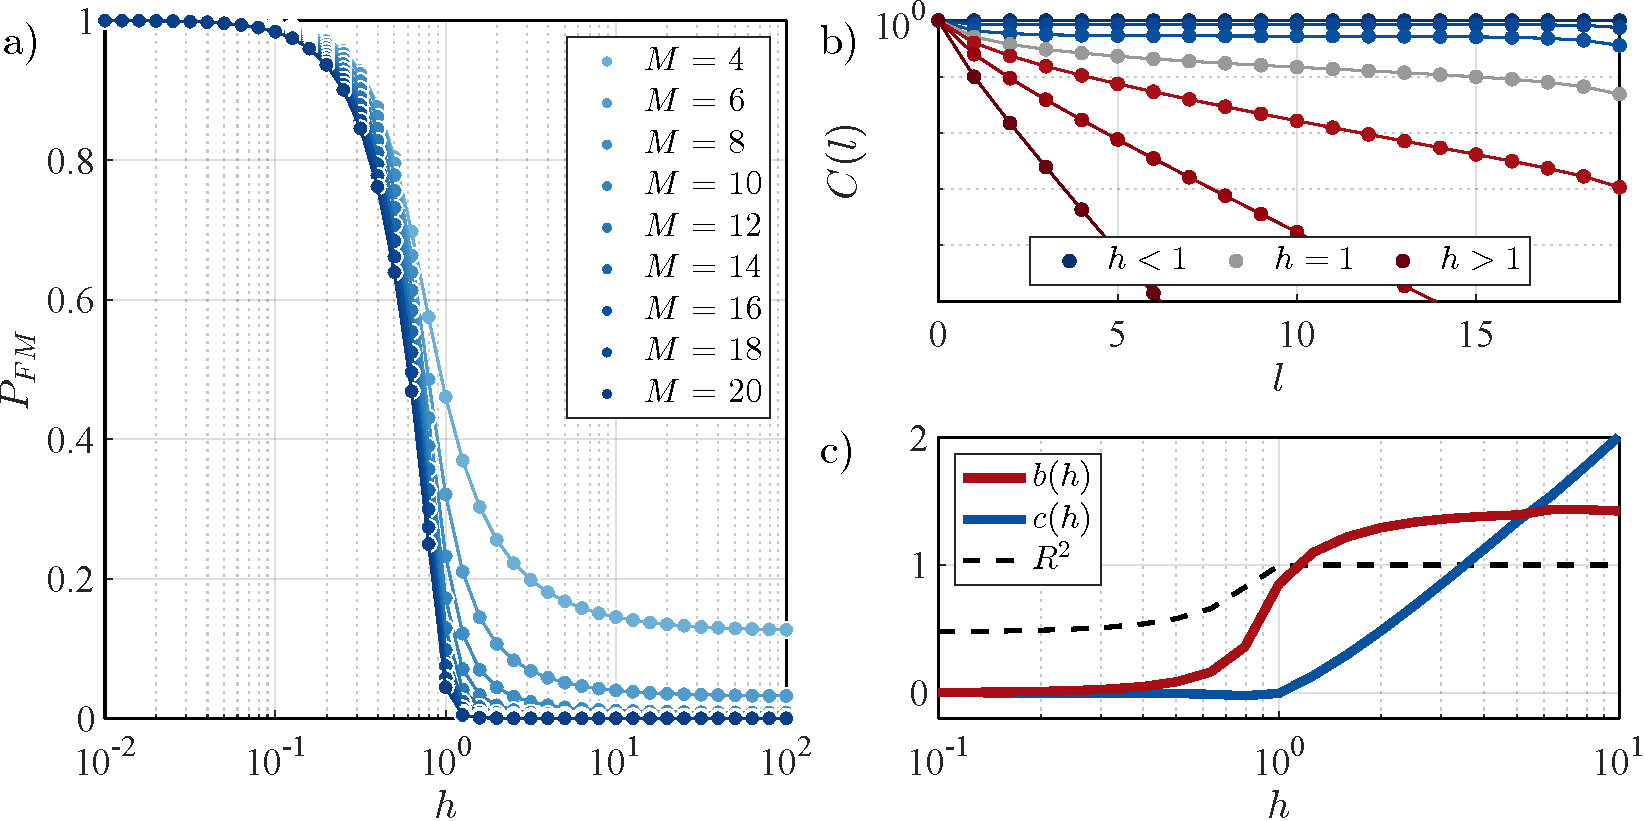
\includegraphics[width=\textwidth]{Chapters/Plots/Chapter2/Chapter1_Fig1.pdf}
    \caption{a) The ferromagnetic order parameter $P_{FM}$ as a function of the coupling strength $h$ of the external magnetic field for a range of system sizes. b) The correlation function $C(l) = \langle \hat{\sigma}^z_1 \hat{\sigma}^z_{1+l} \rangle$ for $M = 20$. c) The parameters of the fitting function $f(h) = a l^{-b} e^{-c l}$ used to fit the correlation function $C(l)$.} 
    \label{fig:Chapter1_Fig1}
\end{figure}

Correlation functions are another useful tool for investigating phase transitions; they are expectation values of products of operators that measure either temporal or spatial correlations. In the model we are considering, we define the correlation function $C(l) = \langle \hat{\sigma}^z_1 \hat{\sigma}^z_{1+l} \rangle$. For $h = 0$, it is easy to see that $C(l) = 1$ as the ferromagnetic ground state has long-range order \cite{carlin1986}. In the limit where $h \to \infty$, the correlation function will decay exponentially to $0$, i.e., $C(l) \propto \exp(- l/\xi)$, where $\xi$ is the length scale over which correlations decay. Typically, correlation functions near criticality exhibit algebraic decay with distance, and a correlation length $\xi$ that diverges \cite{carr2010}. To verify this, we consider the fitting function $f(h) = a l^{-b} \exp(-c l)$, and show the fitting parameters $b, c$ as a function of $h$ in Fig.~\ref{fig:Chapter1_Fig1}~c). The parameter $a$ is simply a scaling factor and does not offer additional insight in our analysis. For $h < 1$, the fit is not accurate ($R^2 \approx 0.5$), and the fitting function does not accurately describe the behavior of the correlation function. For $h \geq 1$, however, we have good agreement with the fitting function ($R^2 \approx 1$). At $h = 1$, we see that $c = 0$, i.e., the correlation function is purely characterized by the algebraically decaying term $l^{-b}$. As the correlation length $\xi$ is the inverse of the fitting parameter $c$, we see that if $c \to 0$, then $\xi \to \infty$. At the critical point, the correlation length diverges, and correlations are non-zero at all possible length scales; for infinite systems, the state and correlations at the transition point are said to be \textit{scale-invariant} \cite{carr2010, sachdev2011}. For $h > 1$, we see the value for $b$ saturates while $c$ continuously increases with $h$, indicative of the exponential decay taking over the behavior of the correlation function. It is important to note that, while $c=0$ also for $h<0$, and this is due to the bad fit for $h<1$. If we subtract the square of the magnetization $\expval{\hat\sigma^z}$, we would see that the correlation length $\xi$ only diverges at the critical point.

Everything we have seen here serves as an introduction to phase transitions and what we look for to determine their existence and behavior. The phase transitions we analyze in chapters~\ref{chap:MIPT_bosons}-\ref{chap:short_time_dynamics} have a different flavor; however, they result from local measurements in open quantum systems. Regardless, all the tools and characteristics we have seen here will be important as they allow us to characterize quantum phases similarly. Now, we continue with the introduction of open quantum systems and the numerical tools that will enable us to simulate them.

 	\chapter{Numerical Simulations of Open Quantum Systems}
\thispagestyle{empty}
\label{chap:tech_sec}

This chapter gives a brief introduction to the field of open quantum systems and the Gorini–Kossakowski–Sudarshan–Lindblad (GKSL) master equation, an equation at the heart of simulating Markovian open quantum systems. We introduce numerical algorithms that can be employed to simulate the GKSL master equation more efficiently via stochastic methods. As we will see in the following chapters, the study of open quantum systems does not only lead to a more complete description of quantum systems, but it also leads to the emergence of new phenomena, such as dephasing \cite{pichler2010,sarkar2014} and dissipative phase transitions \cite{diehl2008, carmichael2015, kessler2012, minganti2018}. Furthermore, the loss of information to the environment usually describes an undesirable process; however, it can also be used as a tool to control, in a programable way, the state of a system, giving rise to dissipative state engineering \cite{verstraete2009, muller2012, vidanovic2014}. These effects are not accessible in closed systems, rendering open quantum systems an interesting scenario for exploring new phenomena.

\section{Introduction}

When studying a quantum system, we consider its time evolution governed by some Hamiltonian $\hat{H}$ that describes the dynamics of the system. The most general description of a quantum state is given by its density matrix $\hat{\rho}$ whose evolution can be studied to infer how a system behaves in a given model. Considering a closed quantum system, the von Neumann equation prescribes its time evolution,
\begin{equation}
    \frac{d \hat{\rho}}{dt} = -i \hbar [\hat{H}, \hat{\rho}].
\end{equation}

In the case of a time-independent Hamiltonian (and setting $\hbar =1$), the evolution of the density operator is then given by the equation,

\begin{equation}
    \hat{\rho}(t) = e^{-i \hat{H} t} \hat{\rho}(0) e^{i \hat{H} t}.
\end{equation}

In practice, however, one is usually only interested in a small part of the global system, which can interact with the rest of the system. In order to obtain a description of this smaller subsystem in terms of a Schr\"{o}dinger equation, one would need to neglect the effects of its interactions with its environment and assume it to be a closed system. This, however, is not a realistic description since, often, one cannot simply ignore these interactions.

\begin{figure}[h]
    \centering

    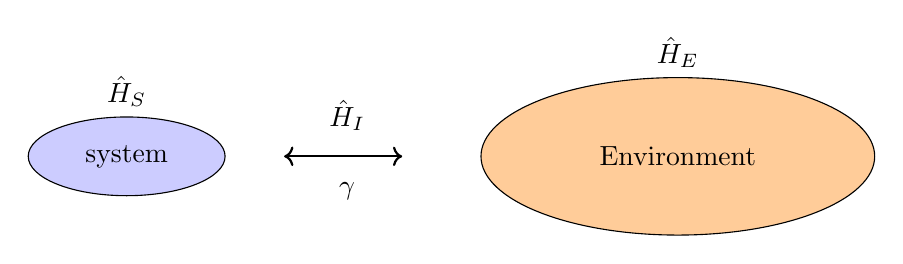
\begin{tikzpicture}
        \node[
            xshift = 0.5cm,
            ellipse,
            draw,fill=blue!20,
            minimum width = 2.5cm,
            minimum height = 1cm,
            label=north: $\hat{H}_{S}$] (sys) at (2,2) {system};
        \node[
            xshift = 7.5cm,
            ellipse,
            draw,
            fill=orange!40,
            minimum width = 5cm,
            minimum height = 2cm,
            label=north: $\hat{H}_{E}$] (env) at (2,2) {Environment};
        \draw[thick,<->] (4.5,2) -- (6,2) node[xshift= -0.7cm,yshift=-0.2cm, anchor=north] {$\gamma$} node[xshift = -0.7cm, yshift = 0.2cm, anchor=south]{$\hat{H}_I$}; 
    \end{tikzpicture}

    \caption{Schematic representation of an open quantum system. The system of interest is coupled to an environment, and the three components describing the overall system are the system Hamiltonian $\hat{H}_S$, the environment Hamiltonian $\hat{H}_E$, and the interaction Hamiltonian $\hat{H}_I$ with coupling rate $\gamma$ between system and environment.}
    \label{fig:Chapter2_Fig1}
\end{figure}

We cannot simply consider the closed system dynamics of the global system, consisting of a system of interest and its environment, due to the exponential scaling of the Hilbert space, which is a difficult problem to solve. This has led to the development of quantum master equations \cite{carmichael1993,breuer2002, manzano2020} to derive equations of motion only for the reduced system (i.e., the system of interest) that account for interactions between the system and its environment but where the environment degrees of freedom have been traced out. Under a set of approximations, which we will discuss later, this leads to a simplified description of only the system of interest, where the effects of the environment on the system are taken into account. 

Without going through the full derivation, we will now introduce the GKSL master equation, perhaps the most well-known master equation, and outline the most important concepts that are at the core of its derivation.

\section{GKSL Master Equation}

As mentioned in the previous section, we will now introduce the GKSL master equation and explain the main ideas behind its derivation. Fig.~\ref{fig:Chapter2_Fig1} shows the schematic representation of the global system $\hat{\rho}_{SE}$ that we are considering; we have the system of interest $\hat{\rho}_S$ with Hamiltonian $\hat{H}_S$, the environment $\hat{\rho}_E$ with Hamiltonian $\hat{H}_E$, and the interaction between system and environment is described by the Hamiltonian $\hat{H}_I$. We combine these components and obtain the global Hamiltonian:
\begin{equation}
    \hat{H} = \hat{H}_S + \hat{H}_E + \hat{H}_I.
\end{equation}

Now, we can write down the time evolution of this global system using the von Neumann equation for density operators, 
\begin{equation}
\label{eq:schr_eq}
    \frac{d}{dt} \hat{\rho}_{SE} = -i [\hat{H}_S+\hat{H}_E+\hat{H}_I, \hat{\rho}_{SE}].
\end{equation}

We then move to the interaction picture by defining the unitary transformations, 
\begin{equation}
\begin{aligned}
    \hat{H}_I(t) = e^{i (\hat{H}_S+\hat{H}_E)t} \hat{H}_I e^{-i (\hat{H}_S+\hat{H}_E)t},\\
    \hat{\rho}_{SE}(t) = e^{i (\hat{H}_S+\hat{H}_E)t} \hat{\rho}_{SE} e^{-i (\hat{H}_S+\hat{H}_E)t},
\end{aligned}
\end{equation}

which allows us to rewrite Eq.~\ref{eq:schr_eq} as:
\begin{equation}
\label{eq:schr_eq_se}
    \frac{d}{dt} \hat{\rho}_{SE}(t) = -i [\hat{H}_I(t), \hat{\rho}_{SE}(t)],
\end{equation}
where we have now introduced the explicit time dependence. As we are interested in the density operator time evolution, we integrate the right-hand side to transform this equation further and obtain, 
\begin{equation}
    \hat{\rho}_{SE}(t) = \hat{\rho}_{SE}(t_0) - i \int_{t_0}^t dt' [\hat{H}_I(t'),\hat{\rho}_{SE}(t')].
\end{equation}

Substituting this expression back into Eq.~\ref{eq:schr_eq_se} we arrive at the following equation, 
\begin{equation}
\label{eq:integro_diff}
    \frac{d}{dt} \hat{\rho}_{SE}(t) = -i [\hat{H}_I(t),\hat{\rho}_{SE}(t_0)] - \int_{t0}^t dt' \big[\hat{H}_I(t), [\hat{H}_I(t'),\hat{\rho}_{SE}(t')]\big]
\end{equation}

As we wish to describe the time evolution of our physical system $\hat{\rho}_S = \Tr_E[\hat{\rho}_{SE}]$, we compute the partial trace over the environment degrees of freedom. Furthermore, we can set the first term to $0$ by choosing an interaction Hamiltonian of the form $\hat{H}_I = \sum\limits_j \hat{S}_j \otimes \hat{E}_j$, where $\hat{S}, \hat{E}$ act on system and environment respectively, and making two assumptions; firstly, that the initial states of the environment and system are not correlated, $\hat{\rho}_{SE}(t_0) = \hat{\rho}_S \otimes\hat{\rho}_E$, and secondly that the initial state of the environment is thermal, $\hat{\rho}_E(t_0) = \exp(- H_E/T)/\Tr[\exp(- H_E/T)]$ with temperature $T$ and setting the Boltzmann constant $k_B=1$. As a result, we can write,
\begin{equation}
\label{eq:integro_diff_trace}
\frac{d}{dt} \hat{\rho}_S(t) = - \int_{t_0}^{t} dt' \Tr_E\big(\big[\hat{H}_ I(t), [\hat{H}_I(t'),\hat{\rho}_{SE}(t')]\big]\big).
\end{equation}
However, having applied the partial trace operator to Eq.~\ref{eq:integro_diff} has not removed the explicit dependence on the global density operator $\hat{\rho}_{SE}$. Furthermore, as it stands now, this expression is exact but very complicated and too difficult to solve analytically or numerically in most cases. For this reason, we will make three approximations, known jointly as the \textit{Born-Markov approximation}, which will allow us to reduce the complexity of this equation heavily. 

\textbf{Born approximation}

The Born approximation assumes that the coupling between the system and environment is weak, which is a valid approximation in many quantum optical systems. The condition is met by simply including all degrees of freedom in the system that strongly interact with each other. Weakly interacting degrees of freedom are kept as the environment. Physically, this means the environment is only minimally affected by interactions with the system, and the system and environment are not entangled. We, therefore, can approximate the total density operator as the tensor product,
\begin{equation}
    \hat{\rho}_{SE}(t) = \hat{\rho}_S(t) \otimes \hat{\rho}_E.
\end{equation}

\textbf{Markov approximation}

The Markov approximation assumes that the time evolution of the system only depends on its current state and has no memory of its past evolution. This means we assume the effects of the interactions between the system and the environment dissipate quickly, and the environment returns back to its equilibrium state to remain approximately static as assumed by the Born approximation. Given the relaxation timescales of the system $\tau_R$ and environment $\tau_E$ for the Markov approximation to hold, we need $\tau_E \ll \tau_R$.

As we have assumed the rapid decay of the environment correlation functions, we can choose $t_0 = 0$ for further simplification and extend the integral from $t$ to $\infty$, which we may do without changing the result.

Applying this together with the \textit{Born-Markov} approximation to Eq.~\ref{eq:integro_diff_trace} we obtain a Markovian master equation, 
\begin{equation}
    \label{eq:born-markov_meq}
\frac{d}{dt} \hat{\rho}_S(t) = - \int_{0}^{\infty} dt' \Tr_E\big(\big[\hat{H}_ I(t), [\hat{H}_I(t'),\hat{\rho}_S(t)\otimes \hat{\rho}_E]\big]\big).
\end{equation}

This equation, also known as the Redfield equation, is trace-preserving but does not guarantee positivity. In order to obtain the GKSL form of the master equation, we need to apply one more approximation, namely the \textit{rotating-wave} approximation. 

\textbf{Rotating-wave approximation}
Let us introduce a general interaction Hamiltonian which can be written in the so-called linear coupling form, 
\begin{align}
    \hat{H}_I(t) &=  \sum_{i,j} \sum_{k}  \Big(\hat{c}_i(t) + \hat{c}^\dagger_i(t)\Big) \Big(\hat{b}_{j,k}(t) + \hat{b}_{j,k}(t)\Big)\\
    &= \sum_{i,j} \sum_{k} (\hat{c}_i(t) \hat{b}_{j,k}(t) + \hat{c}^\dagger_i(t) \hat{b}_{j,k}(t) + \text{h.c.}),
\end{align}
where $\hat{c}_i,\hat{c}^\dagger_i$ denote the system operators, $\hat{b}_{j,k},\hat{b}^\dagger_{j,k}$ denote bosonic environment operators, and h.c. stands for Hermitian conjugate. The index $k$ indicates the sum over the energy modes of the environment, and the Hamiltonian of the environment \cite{gardiner2004} in terms of the bosonic environment operators reads, 
\begin{equation}
    \hat{H}_E = \sum\limits_{j,k} \omega_{j,k} \hat{b}^\dagger_{j,k} \hat{b}_{j,k},
\end{equation}
where $\hat{b}^\dagger_{j,k}, \hat{b}_{j,k}$ satisfiy the bosonic canonical commutation relations.
If we rewrite the operators in the interaction picture, $\hat{c}(t), \hat{b}(t)$ in terms of the Schr\"{o}dinger picture operators $\hat{c}(0), \hat{b}(0)$, we obtain, 
\begin{equation}
\label{eq:int_ham}
    \hat{H}_I(t) = \sum_{i,j} \sum_{k} (\hat{c}_i(0) \hat{b}_{j,k}(0) e^{-i(\omega_i+\omega_{j,k})t} + \hat{c}^\dagger_i(0) \hat{b}_{j,k}(0) e^{-i(\omega_i-\omega_{j,k})t} + \text{h.c.}),
\end{equation}
where $\omega_i, \omega_{j,k}$ are some energy scales of the system and the environment respectively. The rotating wave approximation assumes that these energy scales are approximately equal and we, therefore, obtain two slow-rotating terms $e^{-i(\omega_i-\omega_{j,k})t}$ and two fast-rotating terms, $e^{-i(\omega_i+\omega_{j,k})t}$, and their respective Hermitian conjugates. As the fast-rotating terms oscillate quickly over the typical system relaxation timescale $\tau_R$, they average to zero in this time interval \cite{fujii2017}, and as a consequence, we can omit these terms, which is known as the rotating-wave approximation.
Having described the main approximations used in the derivation of the Markovian master equation, we now present the GKSL form of the master equation, which can be obtained by substituting Eq.~\ref{eq:int_ham} into Eq.~\ref{eq:born-markov_meq}. For the full derivation needed to obtain this form of the master equation, see references \cite{manzano2020}.

\textbf{GKSL master equation}

\begin{equation}
\label{eq:GKSL_meq}
    \dot{\hat{\rho}} = -i [\hat{H}, \hat{\rho}] - \sum_i \frac{\gamma_i}{2} ( \{ \hat{c}^\dagger_i \hat{c}_i, \hat{\rho} \} - 2 \hat{c}_i \hat{\rho} \hat{c}^\dagger_i), 
\end{equation}
where $H$ describes the system Hamiltonian, $\hat{\rho}$ is the system density operator (The subscript \textit{S} has been omitted as we have traced out all environment degrees of freedom, so all operators are now referring to the system.). The operators $\hat{c}_i$ are known as the \textit{Lindblad}, or \textit{jump} operators acting on the $i$-th dissipation channel in a many-body system and describe the type of dissipation that is being simulated in some model of interest. The parameter $\gamma_i$ describes the strength of the dissipation and at what rate energy is being exchanged with the environment. 

We can see from this equation that the first term describes the coherent closed-system time evolution, and the second term describes the resulting dynamics in the system stemming from interactions with the environment, without the need to also simulate the environment and its interactions with the system in a larger Hilbert space. This equation can be solved in many cases for limited system sizes; however, we will now proceed and describe other methods that simulate the GKSL master equation \textit{stochastically}, at the level of the pure vector state instead of the density operator, reducing the dimension of the objects to be simulated, leading to the powerful tool of \textit{quantum trajectories}.

One interesting aspect is that the GKSL Master Equation provides flexibility in choosing jump operators, allowing different sets of related operators to produce the same overall behavior. In contrast, for MIPTs, the choice of operator sets has a clear physical meaning and could lead to different phase transitions. However, even with these differences, the equilibrium state, when averaged over all paths, remains the same.

\section{Quantum Trajectories}

As previously mentioned, we can compute the dynamics of a system coupled to an environment via the GKSL master equation. Numerically, this entails that we need to manipulate and store density operators $\hat{\rho}$, which live in an exponentially large Hilbert space $\mathcal{H}$, represented numerically by matrices consisting of $dim(\mathcal{H})^2$ elements. A pure vector state, however, is numerically represented by a vector consisting of $dim(\mathcal{H})$ elements, which is the motivation behind the so-called \textit{Monte-Carlo} wavefunction method \cite{dum1992, dalibard1992, molmer1993, carmichael1993, plenio1998}, which is a possible choice for the stochastic unraveling of the master equation. This method allows us to simulate the dynamics of the density operator under the GKSL master equation, as in Eq.~\ref{eq:GKSL_meq}, by time-evolving pure states $\{\ket{\psi_i(t)}\}_i$ (with $dim(\mathcal{H}) = 2^M$), sampled from an initial state $\hat{\rho}(t=0)$ and using them to compute individual random trajectories whose statistical averages recover the master equation. Given enough trajectories we can then write $\hat{\rho}(t) = \overline{\ket{\psi(t)}\bra{\psi(t)}}$, where $\overline{\cdot\cdot\cdot}$ denotes the stochastic average over trajectories. This method can be more efficient than the direct simulation of the master equation involving the density operator, as only $dim(\mathcal{H})$ coefficients are required to store a single pure vector state instead of $dim(\mathcal{H})^2$. Still, we must bear in mind that this comes at the cost of having to sample many trajectories to minimize statistical errors, but this is a less restrictive problem as many trajectories can be run in parallel. In the following two sections, we will discuss first-order and higher-order methods, how they are implemented concretely, and how they can be interpreted physically. 

\subsection{First-Order Method}

To obtain a first-order trajectory method, we begin by defining the non-Hermitian effective Hamiltonian,

\begin{equation}
	\label{eq:heff}
	\Heff = \hat{H} - i  \frac{\gamma}{2} \sum\limits_i \hat{c}_i^\dagger \hat{c}_i,
\end{equation}

with which we rewrite the GKSL master equation \ref{eq:GKSL_meq},

\begin{equation}
	\label{eq:meq_heff}
	\dot{\hat{\rho}} = -i [\Heff, \hat{\rho}] + \gamma \sum\limits_i \hat{c}_i \hat{\rho} \hat{c}_i^\dagger.
\end{equation}

To simulate an individual trajectory, we sample a pure state $\ket{\psi{(t =0)}}$ from the initial state $\hat{\rho}(t = 0)$.  With this, we are able to set up an iterative algorithm that computes the dynamics under the effective Hamiltonian undergoing random jumps. The state at time $t+ dt$ in first-order reads,
\begin{equation}
	\label{eq:traj_dt}
	\ket{\psi(t+dt)} = (1 - i \Heff dt) \ket{\psi(t)}.
\end{equation}

As we time evolve under a non-Hermitian effective Hamiltonian, the norm decreases, 
	\begin{align}
    \label{eq:dp}
		\braket{\psi(t+dt)} &= \bra{\psi(t)} (1 + i \Heff^\dagger dt)(1- i \Heff dt)  \ket{\psi(t)} \\
		&= 1 - \gamma dt \sum\limits_i  \bra{\psi(t)} \hat{c}^\dagger_i \hat{c}_i  \ket{\psi(t)} \equiv 1 - \sum\limits_i \delta p_i = 1 - \delta p,
	\end{align}
where the $\delta p_i$ can be seen as the probabilities with which a jump, described by the operator $\hat{c}_i$ will occur in the time interval between $t$ and $t+dt$. 
After propagating the state under the effective Hamiltonian, we make a stochastic selection,
\begin{itemize}
	\item with probability $1-\delta p$, we renormalize the state:
	\begin{equation}
		\ket{\psi(t+dt)} = \frac{	\ket{\psi(t+dt)} }{\sqrt{\delta p}},
	\end{equation}
\item and with probability $\delta p$ a jump occurs:
	\begin{equation}
		\label{eq:jump}
	\ket{\psi(t+dt)} = \frac{	\hat{c}_i \ket{\psi(t)} }{\sqrt{\delta p_i/dt}},
	\end{equation}
where we choose $\hat{c}_i$ randomly according to to the probabilities $\Pi_i = \delta p_i/\delta p$. 
\end{itemize}
This procedure is then repeated to compute the time evolution for a single trajectory until we reach some desired final time $T$.

\begin{mylisting}
    function trajectory(psi0, c, dt, time, Heff)
        psi_t = psi0; % Initialize \psi(t) 
        for t = 1:length(time)-1
            psi_t = (id-1i*dt*Heff)* psi_t; % compute \psi(t+dt) 
            dp = 1-norm(psi_t)^2; % compute jump probability
            if rand < dp 
                % determine where to apply the jump operator
                l = randomJump(psi_t); 
                psi_t = c{l}*psi_t; % apply jump operator
            end
            psi_t = psi_t/norm(psi_t); % renormalize
            % calculate and save observables here
        end
    end
\end{mylisting}    

This pseudocode outlines the described procedure, we have the initial state $\texttt{psi0}$, the array $\texttt{c}$ containing the jump operators $\hat{c}_i$ in position $i$, the numerical time step $\texttt{dt}$, time vector $\texttt{time}$, and the effective Hamiltonian $\texttt{Heff}$. We first initialize a temporary variable containing the initial state and use it in the first time step to compute the state at time $t+dt$ according to Eq.~\ref{eq:traj_dt}. We then compute the jump probability and generate a random number that is uniformly distributed between $0$ and $1$. If it is less than the jump probability we apply a jump operator at a random site $l$. To determine $l$ using $\texttt{randomJump}$, we compute $\Pi_i = \delta p_i/\delta p$ as mentioned above and we define intervals between $0$ and $1$ whose size is proportional to $\delta p_i$. We then draw again a random uniformly distributed number between $0$ and $1$ and pick the index $l$ of the interval in which the random number lies. After this step, we simply renormalize and compute observables or save the state at time $t+dt$ before repeating it until the final simulation time is reached. This has to be then repeated for a large number of trajectories, and upon averaging over many trajectories, we are able to recover the time evolution under the GKSL master equation \ref{eq:GKSL_meq}, which we will prove in the next paragraph.

\textbf{Recovery of the master equation:}

To demonstrate that this stochastic method is equivalent to the master equation \ref{eq:meq_heff} let us consider the density operator of a pure state at a time $t$,
\begin{equation}
 	\hat{\rho}(t) = \ket{\psi(t)} \bra{\psi(t)}.
\end{equation}
As described in the algorithm, with probability $1-\delta p$, we choose the renormalized state, and with probability $\delta p$, we choose the state where a jump occurred. Then, the averaged density matrix at time $t+\delta t$ will be given by the following average,
\begin{equation}
	\overline{\hat{\rho}(t+dt)} = (1-\delta p) \frac{\ket{\psi(t+dt)} \bra{\psi(t+dt)}}{1-\delta p} + \delta p \sum\limits_i \frac{\delta p_i}{\delta p}  \frac{ \hat{c}_i \ket{\psi(t)} \bra{\psi(t)}\hat{c}^\dagger_i}{\delta p_i/dt},
\end{equation}
where $\overline{\hat{\rho}}$ denotes a statistical trajectory average for a given $\hat{\rho}$. With the above definition in equation~\ref{eq:traj_dt} the first term yields: 
\begin{align}
	\ket{\psi(t+dt)} \bra{\psi(t+dt)} &= (1- i dt \Heff ) \ket{\psi(t)} \bra{\psi(t)} (1+ i dt \Heff^\dagger ) \\
	&= (\ket{\psi(t)} - i dt \Heff \ket{\psi(t)} ) (\bra{\psi(t)} - i dt \bra{\psi(t)} \Heff) \\
	&= \hat{\rho}(t) - i dt (\Heff \hat{\rho}(t) - \hat{\rho}(t) \Heff^\dagger),
\end{align}
where in the last line, we omit terms that are not linear in $dt$. 
We obtain: 
\begin{equation}
	\overline{\hat{\rho}(t+dt)} = \hat{\rho}(t) - i dt (\Heff \hat{\rho}(t) - \hat{\rho}(t) \Heff^\dagger)+ dt \sum\limits_i  \hat{c}_i \hat{\rho}(t) \hat{c}^\dagger_i,
\end{equation}
which is equivalent to the Markovian master equation \ref{eq:meq_heff} in a single time step $dt$. Hence we have shown that the algorithm described in this section recovers the evolution under the master equation upon trajectory averaging. 

\subsection{Higher-Order Method}
\label{subsec:higher_order}
In the previous section, we have seen a first-order quantum trajectory method, which time evolves the state using a first-order Taylor expansion of the application of the evolution operator. We can improve the accuracy of this, at the cost of computing a matrix exponential of the effective Hamiltonian, by time evolving via, 
\begin{equation}
	\ket{\psi(t+dt)} = e^{- i \Heff dt} \ket{\psi(t)},
\end{equation}
and then applying the jumps as previously discussed. Computationally, in comparison to before, this step is more costly to perform, as here, the matrix exponential needs to be evaluated. This, however, can be circumvented by using the sparsity of the Hamiltonian or by using functions that compute the action of the exponential operator on the state, see, e.g., Ref.~\cite{expv}. This does not circumvent the fact that jumps require a full time step, leading to an underestimation of the rate at which jumps occur. This can be improved by considering a method that allows the computation of the jump times with arbitrary precision. We start the routine as described in the previous section by sampling a pure state from the initial state $\hat{\rho}(t=0)$. 

We then solve the following equation numerically or analytically for $t_{i+1}$,
\begin{equation}
\label{eq:jumptime}
	||e^{-i \Heff t_{i+1}} \ket{\psi(t_i)} ||^2 = r,
\end{equation}
where $r$ is a uniformly distributed random number between 0 and 1 and $t_{i+1}$ is the time at which the next jump will occur. 
We then compute the time evolution of the state for the time interval $t \in [t_i, t_{i+1}]$ via
\begin{equation}
	\ket{\psi(t)} = \frac{1}{N}  e^{- i \Heff (t -t_i)} \ket{\psi(t_i)},
\end{equation}
with normalization factor: $N = || e^{- i \Heff (t -t_i)} \ket{\psi(t_i)} ||$.

At the time $t = t_{i+1}$, we then apply the quantum jump in the same fashion as described in Eq.~\ref{eq:jump},
	\begin{equation}
	\label{eq:jump_higher}
	\ket{\psi(t_{i+1})} = \frac{	\hat{c}_i \ket{\psi(t_{i+1})} }{\sqrt{\delta p_i/dt}}.
	\end{equation}

As for the first-order method, we repeat these steps to compute the time evolution over the desired time-interval and compute many trajectories over which we compute statistical averages to recover the evolution of the density operator $\hat{\rho}$ under the GKSL master equation \ref{eq:GKSL_meq}. 

Computationally, this method only differs minimally from the previously outlined pseudocode here rather than time evolving with a constant time step throughout the whole simulation, we can numerically solve the exact time at which the jump occurs with arbitrary precision and use any time step we wish, so long as we can accurately compute the state at some time $t$. If, for example, we time evolve a system in the time interval $t\in[0,1]$ using a numerical time step of $dt=0.1$, we have a total of 10 iterations to reach the final simulation time. If at $t=0.35$ a jump occurs, using the first-order method, we will not apply the jump until we reach the time $dt=0.4$. To apply the jump at the exact time it is supposed to occur, we would need to consider a time step of $dt=0.01$, which would require $100$ iterations to reach the final simulation time. Using the higher-order method to compute the jump time exactly and use the numerical time step $dt=0.1$ until we reach the step before the jump, then decrease our time step to the difference between the time when the jump happens and the current time, $dt=0.35-0.3=0.05$. We then apply the jump at this time and continue time-evolving until we reach the final simulation time. This way, we achieve the same accuracy as the first-order method but using only $11$ iterations. When the dissipation rate is low, and jumps only rarely occur, the error tends to remain low, rendering the first-order method a good choice for simulations. When the dissipation rate increases, however, the number of jumps will be underestimated, decreasing the accuracy cumulatively as one time evolves. If, for example, the number of jumps happening in this time interval passes $10$, the average time between jumps will be smaller than the numerical time step, as only $10$ time steps are needed to reach the final simulation time. This simple example demonstrates that as the number of jumps increases with the dissipation rate and the average time between jumps decreases, the first-order becomes increasingly inaccurate due to the over-estimation of when the next jump will occur unless one is willing to reduce the time step significantly. Especially in this regime where the dissipation rate is larger, the higher-order method can prove very useful for both efficiency and accuracy. Note that this has completely ignored the fact that the computation of solving when the jump occurs exactly can also be numerically expensive, so one needs to take into account all these considerations when choosing a method. As we will later show, this computation can also be straightforward to perform, providing both immense improvements in accuracy and computation times.

\subsection{Physical Interpretation}

As we have seen, the quantum trajectory method consists of two parts: the time evolution under an effective Hamiltonian and the random application of jump operators, which simulate the dissipative dynamics of the model. To give some physical context to this method, let us consider a simple two-level system that experiences spontaneous emission \cite{cohen1992}. If we drive the system, we will see coherent Rabi oscillations where the population is transferred back and forth between the ground and the excited state. The Hamiltonian describing this system is given by,
\begin{equation}
    \hat{H} = - \frac{\Omega}{2} (\hat{\sigma}_+ + \hat{\sigma}_-) - \Delta \hat{\sigma}_+ \hat{\sigma}_-,
\end{equation}
where $\Omega$ is the Rabi frequency, characterizing the interaction strength between the system and an external oscillating electromagnetic field, $\Delta$ is the detuning from the resonant frequency, and $\hat{\sigma}_+, \hat{\sigma}_-$ are the raising and lowering operators respectively. The master equation describing the dynamics of the system is given by, 
\begin{equation}
    \dot{\hat{\rho}} = -i [\hat{H}, \hat{\rho}] - \frac{\gamma}{2} \big( \{ \hat{\sigma}_+ \hat{\sigma}_-, \hat{\rho} \} - 2 \hat{\sigma}_- \hat{\rho} \hat{\sigma}_+ \big). 
\end{equation}

\begin{figure}[ht]
    \centering
    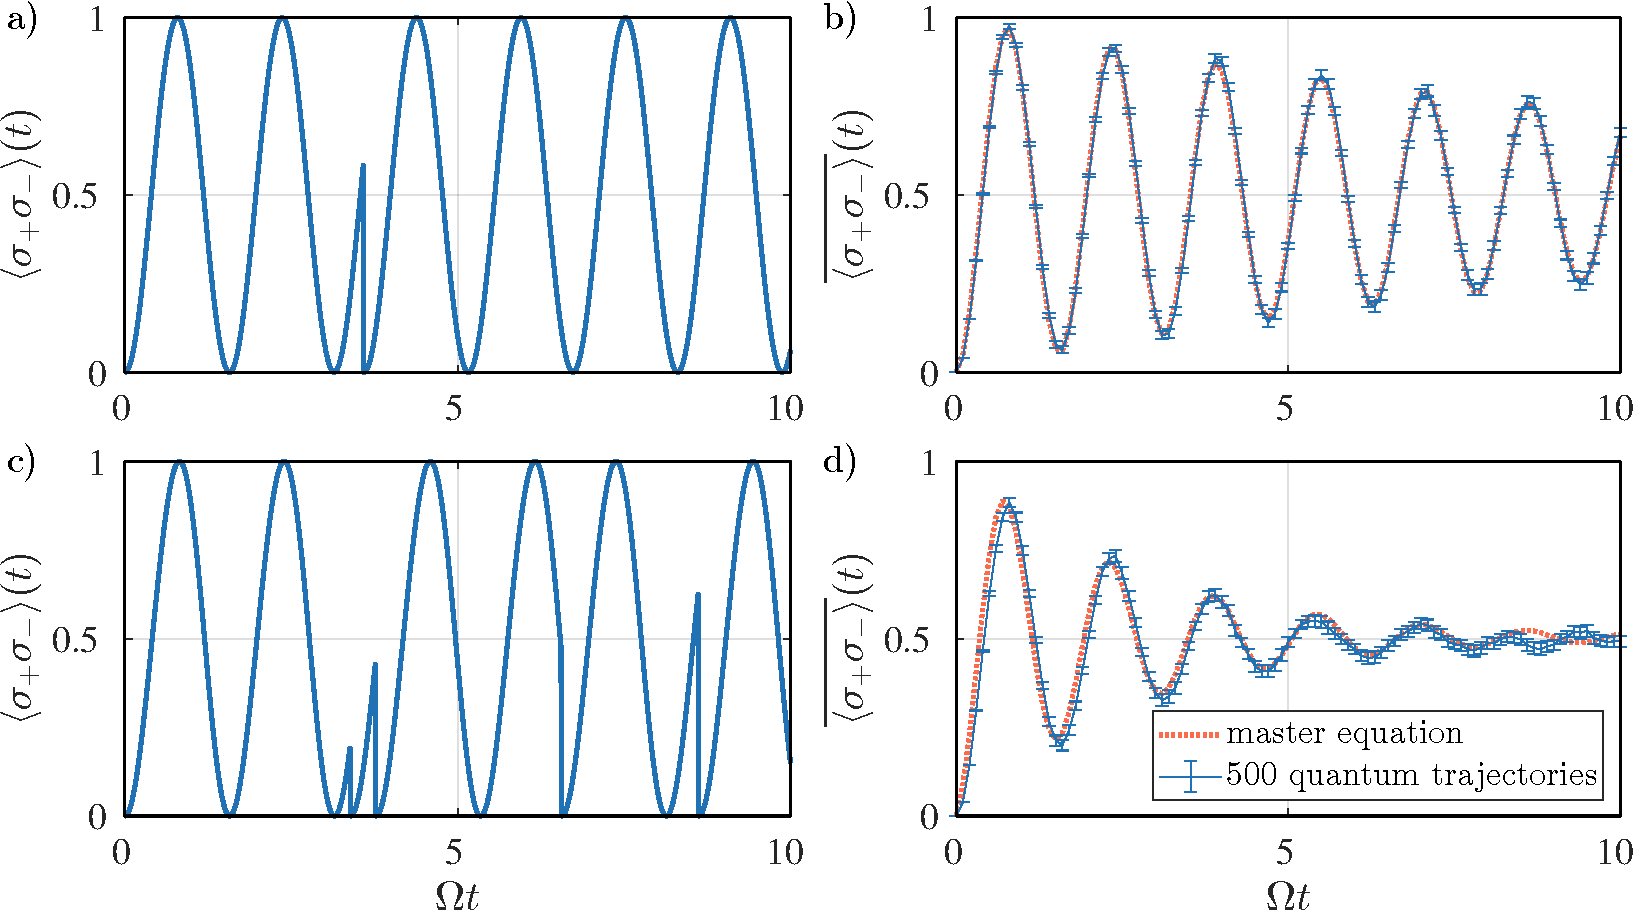
\includegraphics[width=\textwidth]{Chapters/Plots/Chapter3/Chapter2_Fig2.pdf}
    \caption{a), c) Excited state population $\expectation{\hat{\sigma}_+ \hat{\sigma}_-}$ of a two-level system as a function of time in an individual trajectory for two spontaneous decay rates $\gamma = 0.1, 0.5$. Starting from the ground state, the excited state population oscillates coherently at the Rabi frequency $\Omega = 2$ while being interrupted randomly by spontaneous emissions. b), d) Trajectory-averaged excited state population $\overline{\expectation{\hat{\sigma}_+ \hat{\sigma}_-}}$ as a function of time for two spontaneous decay rates $\gamma = 0.1, 0.5$. We compare the quantum trajectory result (blue) to the direct simulation of the master equation (red), where the jump operator is the lowering operator $\hat{\sigma}_-$. We observe good agreement between both methods, using a numerical timestep $dt=10^{-2}$, averaging over $N_t = 500$ trajectories. The statistical errors are computed by dividing the standard deviation of the excited state population by the square root of the number of trajectories \cite{daley2014}.}
    \label{fig:Chapter2_Fig2}
\end{figure}

In Fig.~\ref{fig:Chapter2_Fig2}~a), c) the population of the excited state in a single trajectory is visualized for two spontaneous decay rates $\gamma = 0.1, 0.5$, where the jump operator is the lowering operator $\hat{\sigma}_-$. Starting from the ground state, the system undergoes Rabi oscillations, and we observe the population oscillating between the ground and excited state. Due to spontaneous emission, the atom gets projected into the ground state at random times, and the coherent oscillations are interrupted. With an increasing spontaneous emission rate, we observe the projection into the ground state more frequently. 

In Fig.~\ref{fig:Chapter2_Fig2}~b), d) we display the trajectory-averaged population of the excited state and observe that the quantum trajectory method (blue) recovers the expected dynamics from the master equation (red). An increase in the spontaneous emission rate leads to a stronger damping of the population of the excited state. This example illustrates how individual trajectories can be physically interpreted. The jumps that are randomly applied during the evolution correspond to a sequence of spontaneous emission events that interrupt the coherent dynamics, and if we were to measure the environment, we would gain knowledge that the system was projected into the ground state whenever a photon is detected. In contrast, the time evolution under the effective Hamiltonian corresponds to the coherent dynamics, during which the system undergoes Rabi oscillations. Averaging over many trajectories, we recover the evolution prescribed by the GKSL master equation, where we see the damping effect of the Rabi oscillations caused by spontaneous emissions.

From Fig.~\ref{fig:Chapter2_Fig2}~a), c) we observe at the trajectory level that the number of spontaneous emissions increases with the decay rate. Therefore, the probability of finding the state in the excited state decreases due to an increasing number of projections to the ground state. After some time, $\delta t$, the probability of finding the atom in the excited state is $P_e = \dfrac{\Omega^2 \delta t^2}{4}$. If the decay rate is increased, the number of jumps increases, and the average time $\delta t$ between jumps decreases, and as a consequence, the probability of finding the state in the excited state decreases. This phenomenon, referred to as the \textit{quantum Zeno effect} was first discovered by Itano et al. \cite{itano1990} and is characterized by its tendency to suppress coherent processes, illustrated explicitly in this context by the inhibition of Rabi oscillations. One important point to note is that the equivalence between the Lindblad master equation and the quantum trajectory method is valid for arbitrary decay rates. When increasing the decay rate in numerical simulations, one has to ensure that the numerical parameters are chosen appropriately and that the trajectory-averaged dynamics still coincide with the dynamics resulting from the master equation. Physically, however, the Markov approximation assumes that the environment returns rapidly back to its equilibrium state after being excited, and, therefore, the spontaneous decay rate cannot be increased arbitrarily. At some point, the necessary separation between energy scales is no longer present, and the Markov approximation no longer holds. This means that although the equations themselves do not break, there comes a point where they no longer accurately describe the model that is initially considered.

The unraveling of the master equation we have discussed here is not unique, and in the next section, we will introduce another method, known as \textit{quantum state diffusion} relating to quantum measurement theory. These methods were developed around the same time \cite{gisin1992} as the quantum jump approaches and entail a different physical interpretation, which we will discuss as well. Rather than jump processes that model the dissipative dynamics, a stochastic Schr\"{o}dinger equation approach is used with random noise to model the incoherent dynamics.

\section{Homodyne Detection and Quantum State Diffusion}

As mentioned, the previous quantum jump approach is not a unique unraveling of the master equation, and we can write down other quantum trajectory methods. One such method, known as \textit{quantum state diffusion}, is the result of the analysis of stochastic differential equations and was first derived by \cite{gisin1992,wiseman1993}. We will discuss this further in chapter \ref{chap:MIPT_continuous_measurement} as this method lies at the heart of our work in that chapter. Instead, we will focus on the mathematical background and present the algorithm. We will also put it in the context of \textit{homodyne detection} to have a physical interpretation of this method.

\subsection{Quantum State Diffusion}
\label{subsec:qsd}
The GKSL master equation, Eq.~\ref{eq:GKSL_meq}, can be rewritten as a stochastic differential equation for a pure state $\ket{\psi}$, which is known as \textit{quantum state diffusion}. The following stochastic Schr\"{o}dinger equation (SSE) simulates the dynamics of a single trajectory,

\begin{align}
\label{eq:schr_sse}
\begin{split}
    \ket{\psi(t+dt)} &= \big[ 1 - i \hat{H} - \frac{\gamma}{2} \sum\limits_i \hat{c}^\dagger_i \hat{c}_i \big] \ket{\psi(t)} dt \\ 
&+ \big[ \sum\limits_i \frac{\gamma}{2} \expval{\hat{c}_i+\hat{c}^\dagger_i} \hat{c}_i + \sqrt{\gamma} \hat{c}_i \frac{dW_i(t)}{dt} \big] \ket{\psi(t)} dt,
\end{split}
\end{align}
where $\hat{c}_i,\hat{c}^\dagger_i$ are the jump operators, $dW_i(t)$ is a Wiener increment in It\^o form \cite{wiseman2009} and leads to a noisy output signal, which we further discuss in the next sections. Furthermore, the Wiener increment is not correlated in time or with other sites in the system, which we formally express as, 
\begin{align}
\begin{split}
\label{eq:noise}
        E[dW_i(t)] &= 0 \\
        E[dW_i(t) dW_j(t')] &= dt \delta_{i,j} \delta_{t,t'}.
\end{split}
\end{align}

Note that Eq.~\ref{eq:schr_sse} yields an unnormalized state, so in numerical simulations, one must explicitly normalize in each time step. Furthermore, this equation shows how the time evolution of the state at time $t+dt$ is conditioned on the expectation value of the observable $\expval{\hat{c}_i+\hat{c}^\dagger_i}$ at time $t$. This measurement corresponds to measuring the $x$ quadrature of the system, with the $x$ quadrature operator defined as $\hat{x} = \hat{c}+\hat{c}^\dagger$. This naturally emerges when considering a homodyne detection scheme, which is the topic of the next section. 

\subsection{Homodyne Detection}
\label{subsec:hom_detec}

Homodyne detection is a scheme where an output signal of a system of interest and a local strong oscillator field are mixed in a low-reflectivity beamsplitter (LRBS), as can be seen in Fig.~\ref{fig:Chapter2_Fig3}. The output signal gets recorded by a photodetector and is proportional to the homodyne current $J_\text{hom}$, in which the $x$ quadrature of the system output field is encoded. To see why this is the case, we will provide a brief derivation for the case of \textit{balanced homodyne detection} at the end of this section.

\begin{figure}[ht]
    \centering
    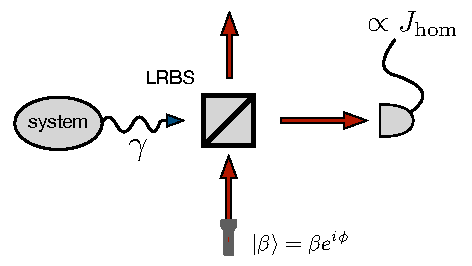
\includegraphics[width=9cm]{Chapters/Plots/Chapter3/Chapter2_Fig3.pdf}
    \caption{A schematic representation of the homodyne detection scheme. The system output signal is mixed in a low reflectivity ($R \to 0$) beamsplitter with a strong local oscillator. The state of the local oscillator is given by $\ket{\beta} = \beta e^{i \phi}$, where $\beta$ is the amplitude and $\phi$ the phase of the oscillator.}
    \label{fig:Chapter2_Fig3}
\end{figure}

Intuitively, we can think of this setup as mixing an unknown signal with a reference signal, allowing us to learn about the unknown system signal, but only weakly probing it and not fully collapsing the system wavefunction. As atoms have the ability to relax through fluorescence, they can emit photons into their electromagnetic environment. In experiments through detecting and counting the emitted photons, discrete quantum jumps of the state can be observed, collapsing the system wavefunction as we saw in the previous section. If, instead, the amplitude of the fluorescence field is mixed coherently with a local oscillator by a beamsplitter, then each realization of a measurement record can be used to construct a quantum trajectory whose evolution obeys quantum state diffusion, and a homodyne current can be measured. This is related to chapter \ref{chap:MIPT_continuous_measurement} where we consider a system of free fermions and use the homodyne current that arises in such a setup to investigate the measurement-induced phase transition that arises in this model. As we will discuss later, the local oscillator also amplifies the system output signal, so this setup is also useful when the output from the system is weak.

In this setup, only the transmitted signal is recorded in a photodetector, and although a low-reflectivity beamsplitter is used, some of the system signal will be reflected and lost. To counteract this, the local oscillator $\beta$ amplitude must be large. To completely avoid the loss of signal, we need the reflectivity $R$ of the beamsplitter to go to zero ($R \to 0$), which in turn means the amplitude $\beta$ of the local oscillator needs to be infinite ($\beta \to \infty$). In this limit, the photodetection rate goes to infinity, but as the local oscillator dominates the recorded signal, the effect on the system goes to zero. This means the collapses that the system experiences due to the measurement process become infinitesimally small; however, they happen at an infinite rate, leading to a continuous evolution in time of the conditioned state of the system. As individual collapses only affect the state of the system infinitesimally, the photocurrent at the detector needs to be integrated over a time interval $\Delta T$, chosen such that $\Delta T$ is small compared to times over which the system changes significantly, but large enough to have witnessed a large number of collapses. This treatment leads us to the approach of describing this setup using a stochastic Schr\"{o}dinger equation (SSE) (Eq.~\ref{eq:schr_sse}), and full derivations of this can be found in Refs.~\cite{carmichael1993}.

\textbf{Balanced Homodyne Detection}
Homodyne detection has proven to be a useful setup for measuring the dynamics of a system state that is conditioned on its measurements. Balanced homodyne detection (BHD) works similarly, and its setup is shown schematically in Fig.~\ref{fig:Chapter2_Fig4}.

\begin{figure}[ht]
    \centering
    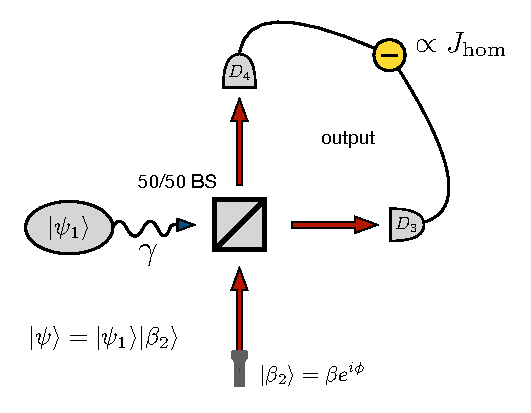
\includegraphics[width=9cm]{Chapters/Plots/Chapter3/Chapter2_Fig4.pdf}
    \caption{The homodyne detection setup consists of a $50/50$ beamsplitter, which mixes the system output equally with a strong local oscillator. The two output beams are then subtracted, and the resulting signal is proportional to the homodyne current $J_\text{hom}$.}
    \label{fig:Chapter2_Fig4}
\end{figure}

Instead of using an LRBS, a $50/50$ beamsplitter is used instead. The two equally mixed output signals are recorded in photodetectors and subtracted from one another, yielding the output signal. Due to the subtraction of the two signals, noise and fluctuations arising in this setup are canceled out as they often originate from the same source, resulting in BHD being the preferred setup. 

In order to find an expression for the current, let us consider some pure system state $\ket{\psi}_1$, and the local oscillator to be simply a coherent state $\ket{\beta}_2 = \beta e^{i \phi}$. The joint input state then is $\ket{\psi}_\text{in} = \ket{\psi}_1 \ket{\beta}_2$. The photocurrents that are measured on detectors $D_3, D_4$ will be proportional to the expectation value of the respective number operators $\hat{n}_i = \hat{c}^\dagger_i \hat{c}_i$ ($i = 3,4$), where $\hat{c}^\dagger_i, \hat{c}_i$ are the respective raising and lowering operators. We consider a $50/50$ beamsplitter so we have transmittivity $T = \frac{1}{\sqrt{2}}$ and reflectivity $R = \frac{1}{\sqrt{2}}i$ and with this we can rewrite the operators as $\hat{c}_3 = T \hat{c}_1 + R \hat{c}_2$ and $\hat{c}_4 = R \hat{c}_1 + T \hat{c}_2$. 
With some algebra, we can express the difference $\hat{n}_3-\hat{n}_4$ as, 
\begin{align*}
    \hat{n}_3 - \hat{n}_4 &= \hat{c}^\dagger_3 \hat{c}_3 - \hat{c}^\dagger_4 \hat{c}_4   \\
    &= \frac{1}{2} \big[ (\hat{c}^\dagger_1 - i \hat{c}^\dagger_2)(\hat{c}_1 + i\hat{c}_2) - (\hat{c}^\dagger_2 - i \hat{c}^\dagger_1)(\hat{c}_2 + i \hat{c}_1) \big]\\
    &= 2 \big[\frac{1}{2i} (\hat{c}_1 \hat{c}^\dagger_2 - \hat{c}^\dagger_1 \hat{c}_2) \big]. 
\end{align*}
The photocurrent $i_{34} = i_3-i_4$ is proportional to the expectation value of this operator, 
\begin{align*}
    i_3-i_4 & \propto \expval{\hat{n}_3 - \hat{n}_4} \\
    & \propto 2 \bra{\psi} \big[\frac{1}{2i} (\hat{c}_1 \hat{c}^\dagger_2 - \hat{c}^\dagger_1 \hat{c}_2) \big] \ket{\psi} \\
    & \propto 2 \bra{\psi_1} \big[\frac{1}{2i} (\hat{c}_1 \bra{\beta_2}\hat{c}^\dagger_2\ket{\beta_2} - \hat{c}^\dagger_1 \bra{\beta_2}\hat{c}_2\ket{\beta_2}) \big] \ket{\psi_1} \\
    & \propto 2 |\beta| \bra{\psi_1} \big[\frac{1}{2i} (\hat{c}_1 e^{-i \phi} - \hat{c}^\dagger_1 e^{i \phi}) \big] \ket{\psi_1}\\
    & \propto 2 |\beta| \expval{\hat{x}_\phi}_1,
\end{align*}
where $\hat{x}_\phi$ is the generalized quadrature operator. Choosing $\phi = \frac{\pi}{2}$, for example, leads to measuring the $\hat{x}$ quadrature of the system. This simple calculation shows that the subtraction of the two photocurrents leads to a signal that is proportional to the oscillator field amplitude and the measurement of the $\hat{x}$ quadrature of the system for some phase angle $\phi$ of the local oscillator field. BHD leads to the same SSE as in the case of simple homodyne detection, as can be seen in Ref.~\cite{carmichael1993}. To see where the stochastic nature arises from, we can consider a time interval during which the system experiences some number of collapses. These collapses occur randomly in time and can be modelled with a stochastic process. This is why the white noise term appears in the conditioned time evolution of the state. As we consider the limit where the amplitude of the local oscillator goes to infinity ($\beta \to \infty$), the homodyne current becomes a continuous function in time rather than a jump process. The homodyne current is not simply the amplitude of the output signal that we mix with the local oscillator, and it also consists of a white noise term. We define the homodyne current as, 
\begin{equation}
\label{eq:Jhom}
    J_\text{hom} = \frac{\expval{\hat{x}}}{2} + \frac{dW}{\sqrt{\gamma} dt}.
\end{equation}
With this definition we can rewrite the SSE \ref{eq:schr_sse} as, 
\begin{align}
\label{eq:schr_sse_hom}
\begin{split}
    \ket{\psi(t+dt)} &= \big[ 1 - i \hat{H} - \frac{\gamma}{2} \sum\limits_i \hat{c}^\dagger_i \hat{c}_i + \gamma \sum\limits_i J_\text{hom} \hat{c}_i \big] \ket{\psi(t)} dt,
\end{split}
\end{align}
where $J_\text{hom}$ is the current associated to the $\hat{x}$ quadrature operator $\hat{x}_i$. The signal that is picked up by the photodetector is proportional to this homodyne current, and as the white noise term has zero mean, upon averaging over many trajectories, the $\hat{x}$ quadrature of the system output field can be measured. This algorithm is easily implementable and has allowed us to obtain the results presented in chapter~\ref{chap:MIPT_continuous_measurement}.

\section{Fermionic Gaussian States}
\label{sec:FGS}

To conclude our introduction to the numerical tools used in this thesis, we now discuss Fermionic Gaussian States (FGS). These states are fully characterized by their correlation matrix, which we introduce below, substantially simplifying calculations. As mentioned earlier, the density operator that numerically represents a quantum state lives in an exponentially large Hilbert space $\mathcal{H}$. Therefore, it follows that the number of elements needed to store the state numerically also scales exponentially with the number of lattice sites. In contrast, as FGS are completely characterized by their correlation matrix, the number of elements needed for its representation scales with the square of the lattice size. For the simulation of dynamics, FGS have the useful property that they remain Gaussian under time evolution with a quadratic Hamiltonian. This means that the Hamiltonian can only contain quadratic terms in the fermionic raising and lowering operators, which restricts the models we can simulate with them. This section mainly introduces two trajectory algorithms we use to generate the data for chapters~\ref{chap:MIPT_bosons} and \ref{chap:MIPT_continuous_measurement}. The algorithms and methods below are adapted from the following References~\cite{alberton2021,cao2019,surace2022}. 

\subsection{Time evolution with FGS}
For a general Fermionic Quadratic Hamiltonian we write,
\begin{equation}
    \hat{H} = \sum\limits_{i,j} \big(A_{ij} \hat{c}_i^\dagger \hat{c}_j + B_{ij} \hat{c}_i \hat{c}_j \big) + h.c.,
\end{equation}
where $\hat{c}_i^\dagger,\hat{c}_i$ are the fermionic raising and lowering operators acting on site $i$. In this thesis, we only consider number-conserving quadratic Hamiltonians, i.e., $B_{ij} = 0 ~\forall i,j$. $A$ is the hopping matrix and encodes the connections between lattice sites. We parameterize the normalized FGS as follows, 
\begin{equation}
\label{eq:fgs}
\ket{\psi_t} = \prod_{n=1}^N\Big( \sum\limits_{i=1}^M \hat{U}_{i,n}(t) \hat{c}^\dagger_i \Big) \ket{0},
\end{equation}
where $M$ is the number of lattice sites, $N$ is the particle number, and $\hat{U}$ satisfies $\hat{U}^\dagger \hat{U} = \mathbb{I}$. From this parameterization, we compute the correlation matrix, which fully characterizes the FGS,
\begin{equation}
    D_{ij}(t) = \expectation{\hat{c}_i^\dagger \hat{c}_j} = [\hat{U}(t) \hat{U}^\dagger(t)]_{j,i},
\end{equation}
where $\hat{c}_i^\dagger,\hat{c}_i$ are the fermionic raising and lowering operators acting on site $i$. 
Then, the closed system time evolution follows the equation, 
\begin{equation}
\label{eq:timeev}
\hat{U}(t+dt) = e^{-iA dt} \hat{U}(t),
\end{equation}
where $D(t) = [\hat{U}(t)\hat{U}^\dagger(t)]^T$ is the correlation matrix at time $t$, $A$ is the hopping matrix, and $dt$ is the numerical time step.

Finally, for a subsystem $M = [m_i,m_j]$ we can compute the reduced correlation matrix $D_M(t) = D_{m_i,m_j\in M}(t)$. The von Neumann entropy can be computed \cite{surace2022} using,
\begin{equation}
\label{eq:vnE}
S(D_M) = -\sum\limits_{i} \lambda_i \ln\lambda_i + (1-\lambda_i)\ln(1-\lambda_i),
\end{equation}
where $\{\lambda_i\}$ is the spectrum of $D_M$. 

Because FGS are fully characterized by their correlation matrix, we only require $M^2$ to describe a system consisting of $M$ sites fully. Furthermore, as we are also able to calculate the entropy from the correlation matrix, we have efficient methods that we use throughout chapters \ref{chap:MIPT_bosons} and \ref{chap:MIPT_continuous_measurement}.

\subsection{Quantum Jump Algorithm}

To implement the quantum jump algorithm outlined in section \ref{subsec:higher_order}, we use the fact that we are dealing with a number-conserving Hamiltonian, which allows us to compute the times at which quantum jumps occur explicitly. Normally, we would need to solve Eq.~\ref{eq:jumptime} numerically; however, given the total particle number, we can solve this equation explicitly, and the jump times can be computed using, 
\begin{equation}
    t_{i} = t_{i-1} - \frac{\ln{r}}{\gamma N},
\end{equation}
where $t_{i-1}$ is the time when the last jump occurred ($t_0 = 0$), and $r$ is a random number between $0$ and $1$ drawn from a uniform distribution.

We then compute the time evolution of the correlation matrix using Eq.~\ref{eq:timeev} until the first jump occurs. Then, the jump is applied via, 
\begin{equation}
  D_{ij} =
    \begin{cases}
      1, & i = j = k\\
      0, & i \neq j \text{ and } (i = k \text{ or } j = k)\\
      D_{ij} - \frac{D_{kj}D_{ik}}{\expectation{n_k}_t}, & \text{otherwise},
    \end{cases}       
\end{equation}
where $\expectation{n_k}_t$ is the jump operator at site $k$ that has been selected considering the probabilities $p_i$ in Eq.~\ref{eq:dp}. Then, we perform a singular value decomposition, $D = U S U^\dagger$, to obtain a new $U$ matrix, continue time evolving until the next jump, and repeat this process until the end of the simulation.

\subsection{Quantum State Diffusion}

We previously introduced QSD in section~\ref{subsec:qsd}, which we can also simulate efficiently using FGS. This algorithm is generally more efficient as the whole time evolution can be simulated using only the $U$ matrix. We aim to simulate the following stochastic Schr\"{o}dinger equation,
\begin{equation}
\label{eq:SSE}
       \ket{\psi(t+dt} = \Big(1-iH dt + \sum\limits_{i=1}^M\Big[ \sqrt{\gamma} (n_i-\langle n_i\rangle_t) dW_{i,t}- \frac{\gamma}{2} (n_i-\langle n_i\rangle_t)^2 dt\Big]  \Big) \ket{\psi_t},
\end{equation}
which explicitly depends on the expectation value of $n_i(t)$. Note that this expression is equivalent to Eq.~\ref{eq:schr_sse}; however, this equation contains additional normalization terms. Furthermore, the monitored quadrature operator is the local number operator $\hat{c}_i = \hat{n}_i$.  

The time evolution for FGS is implemented using,
\begin{equation}
\label{eq:evol}
U(t+dt) = W e^{-iAdt} U(t),
\end{equation}
where  $W$ is the stochastic matrix $W = \text{diag}(e^{dW_{i,t}+\gamma(2\langle n_i \rangle-1)dt})$, and $A$ is the hopping matrix of the Hamiltonian, $\hat{H} = \sum\limits_{i,j} h_{ij} \hat{c}_i^\dagger \hat{c}_j  + \text{h.c.}$. Here, the factor $\sqrt{\gamma}$ has been absorbed in the white noise term, which now satisfies $E[dW_{i,t}] = 0$ and $E[dW_{i,t}dW_{j,t'}] = \delta_{i,j}\delta(t-t') \gamma dt$. Finally, the normalization of U is enforced via a QR decomposition, $U = QR$, and then redefining $U = Q$, which ensures that $U$ is orthonormal. Then, as with other trajectory algorithms we have discussed, we repeat this process until the final simulation time is reached. 

\section{Summary}

In this chapter, we have introduced the GKSL master equation, which can be used to simulate Markovian open quantum systems. We provided an overview of the derivation and the approximations used to obtain the final form of the equation. We then introduced stochastic unraveling methods of the master equation, namely quantum trajectories, where in individual trajectories, coherent dynamics are interrupted by so-called quantum jumps and quantum state diffusion, where the dynamics of a pure state are governed by a stochastic Schr\"{o}dinger equation. Lastly, we introduce Fermionic Gaussian States (FGS) as a numerical tool to simulate specific models. Specifically, in chapter~\ref{chap:MIPT_bosons}, we use both quantum jump trajectories and quantum state diffusion in combination with FGS to access larger system sizes; in chapter~\ref{chap:MIPT_continuous_measurement}, we use quantum state diffusion and FGS, and lastly, in chapter~\ref{chap:short_time_dynamics} we consider only quantum jump trajectories for limited system sizes.
	
	\chapter{Detection of a Measurement-Induced Phase Transition in Interacting Systems}
\thispagestyle{empty}
\label{chap:MIPT_bosons}

\section{Introduction}

\blfootnote{The content of this chapter consists of work done for a project which started in May 2019. Towards the final stages of finishing this project, we became aware of a preprint by Fuji et al., who independently were working on a very similar project \cite{fuji2020}. For this reason, we decided not to publish our work at the time. Furthermore, we concluded that with our limited system size data, we could not provide any strong claims regarding the precise location of the phase transition, which we will discuss in section \ref{subsec:discussion_scaling}.}

In chapter~\ref{chap:intro}, we introduced the measurement-induced phase transition (MIPT) that was discovered in random circuits \cite{li2018,li2019,skinner2019}, resulting from the competition between entangling unitary dynamics and disentangling local measurements. Qualitative changes in the system wave function characterize these phase transitions as the system undergoes a phase transition from volume-law to area-law scaling of the entropy at a critical measurement strength.

In this section, we study such MIPTs in continuous time systems at long times, which emerge from the competition between coherent time evolution and projective measurements that result from interactions with an environment. We explore a 1D chain of hard-core bosons that can tunnel between neighboring sites, and to break integrability, we include interactions between first and second neighbors. The system experiences on-site dephasing, which can be regarded as the result of an external observer performing projective measurements on the system and losing information to the environment. This could arise physically, for example, due to inelastic light scattering \cite{pichler2010,poletti2013,sarkar2014,luschen2017}. The model is discussed in more detail in the following section. The steady state of this model, at the density operator level, is the trivial infinite temperature state that is reached independent of the measurement strength, therefore masking the transition. To access the transition, we need to consider an unraveling of the master equation where we can study the entanglement properties. To achieve this, we use quantum trajectories and consider non-linear functions of the density operator, which are then averaged over individual measurement outcomes, which are no longer independent of measurement strength, thus revealing the transition.

We find that when the measurement strength is small, quantum correlations spanning the whole system are able to build up, and the volume-law scaling is preserved in the interacting model. For large measurement strengths, however, the system favors a product state where information becomes localized, and the entanglement does not build up. This provides an example of a system where the interplay between unitary and dissipative processes can fundamentally change the nature of the coherent dynamics, giving insights into how the entanglement properties of a system are affected by the coupling to an external reservoir. In the following sections, we will provide an analysis of the entropy scaling forms that emerge from this competition, perform finite size-scaling analysis, and provide conclusions that can be drawn from this analysis.

\section[Interacting Hard-Core Bosons and Free Fermions on a 1D Chain]{Interacting Hard-Core Bosons and Free \\ Fermions on a 1D Chain}

In this chapter, we study a chain of hard-core bosons that hop between neighboring sites, and we include first and second-neighbor interactions to break the integrability of the model. We simulate this model using exact diagonalization (ED) techniques, which heavily limits the system sizes we can access. We use the fact that in 1D, there is a one-to-one correspondence between a system consisting of hard-core bosons and spin-1/2 particles \cite{halperin1986}. Furthermore, spin-1/2 particles can be mapped to non-interacting free fermions via the Jordan-Wigner transformation \cite{nielsen}, 
\begin{align}
\begin{split}    
    \hat{\sigma}_j^+ &= \hat{c}_j^\dagger K_j^+, \\
    \hat{\sigma}_j^- &= \hat{c}_j K_j^-, \\
    \hat{\sigma}_j^z &= \hat{c}_j^\dagger \hat{c}_j - \frac{1}{2},
\end{split}
\end{align}
where $\hat{K}_j^{\pm} = e^{\pm i \pi \sum_{k<j} \hat{n}_k}$ is the string operator, with $n_k = \hat{c}_j^\dagger \hat{c}_i$ the fermionic number operator in site $j$, and $\hat{c}_j^\dagger, \hat{c}_j$ the creation and annihilation operators respectively in site $j$.
This transformation allows us to compare our results in a bosonic system with those in a fermionic system. Free fermions enable efficient simulation of much larger system sizes at the cost of being restricted to only being able to consider the non-interacting case. Nevertheless, this still is a powerful tool that allows us to draw valuable conclusions in this chapter.

\subsection{Model I}
    \begin{figure}[ht]
        \centering
        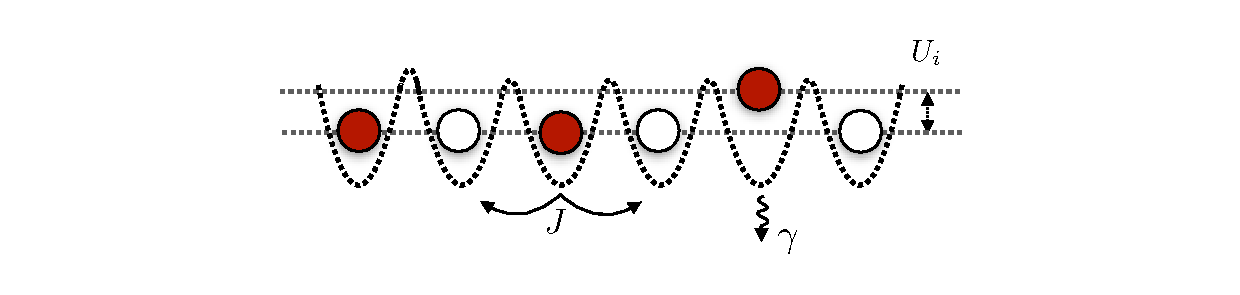
\includegraphics[width = \textwidth]{Chapters/Plots/Chapter4/Chapter3_Fig1.pdf}
        \caption{Schematic representation of a periodic 1D system consisting of hard-core bosons, subject to dissipation. $J$ describes the hopping strength, $U_i$ describes the interaction strength between sites at a distance $i$ and $\gamma$ describes the dissipation strength. We assume periodic boundary conditions, $M+1\equiv 1$, where $M$ is the number of lattice sites.}
        \label{fig:Chapter3_Fig1}
    \end{figure}
    
We consider a periodic 1D chain (Fig.~\ref{fig:Chapter3_Fig1}) that consists of hard-core bosons (particles that cannot occupy the same state, i.e., we have at most one particle per site) with nearest-neighbor hopping and interactions between first and second neighbors to break integrability, described by the system Hamiltonian,
\begin{equation}
\hat{H} =  \hat{H}^b_\text{hop} + \hat{H}_\text{int}.
\end{equation}
The term $\hat{H}^b_\text{hop}$ describes the hopping Hamiltonian,
\begin{equation}
\label{eq:ham}
\hat{H}^b_\text{hop} =-J \sum\limits_{i=1}^{M} ( \hat{a}^{\dagger}_i \hat{a}_{i+1} + \textrm{h.c.}),
\end{equation}
with hopping parameter $J$.  $\hat{a}^\dagger_i, \hat{a}_i$ are the respective bosonic creation and annihilation operators in sites $i$, satisfying the commutation relations, $[a_i,a_j^\dagger] = \delta_{ij}$ and $[a_i,a_j]= [a_i^\dagger, a_j^\dagger] = 0$.

The second term denotes the interaction Hamiltonian,
\begin{equation}
\hat{H}_\text{int} = U_1\sum\limits_{i=1}^{M} \hat{n}_i \hat{n}_{i+1}
+ U_2\sum\limits_{i=1}^{M} \hat{n}_i \hat{n}_{i+2},
\end{equation}
where $U_1$, and $U_2$ are the interaction strengths between first and second neighbors respectively and $\hat{n}_i=\hat{a}_i^\dagger \hat{a}_i$. 

For simulating the dynamics of the fermionic system, we replace the bosonic operators in the Hamiltonian described in Eq.~\ref{eq:ham}, with the fermionic raising and lowering operators, $\hat{c}^\dagger_i, \hat{c}_i$,
\begin{equation}
\hat{H}^f_\text{hop} =-J \sum\limits_{i=1}^{M} ( \hat{c}^{\dagger}_i \hat{c}_{i+1} + \textrm{h.c.}).
\end{equation}
The fermionic operators satisfy the anticommutation relations, $\{c_i,c_j^\dagger\} = \delta_{ij}$ and $\{c_i,c_j\}= \{c_i^\dagger, c_j^\dagger\} = 0$, where $\{a,b\} \equiv ab + ba$ defines the anticommutator.

For both hard-core bosons and FGS, we consider this system subject to dephasing of the local particle numbers, with the number operator $\hat{n}_i$ being the jump operator that models the dissipation. The system dynamics are described by the GKSL master equation (Eq.~\ref{eq:GKSL_meq}). We consider a photon counting unraveling of the master equation to simulate the dynamics and access the phase transition. Due to the conservation of the $U(1)$ symmetry in the model, we can explicitly compute the jump times from Eq.~\ref{eq:jumptime} using $t_{i+1} = -\dfrac{\ln{r}}{\gamma N}$, where $\gamma$ is the measurement strength, $N$ is the total particle number, and $r$ is a random number drawn uniformly from the interval $(0,1)$.

\subsection{Model II}
\label{subsec:model2}
To explore in more detail what can be deduced from Model I, we turn to the secondary model, which consists of the same Hamiltonian, but we substitute the dephasing process with a single particle pump and loss term. We do this to explicitly break the $U(1)$ symmetry associated with excitation number conservation. The resulting GKSL master equation reads, 
\begin{equation}
\label{eq:meqpm}
    \dot{\hat{\rho}} = -i [\hat{H},\hat{\rho}] + \gamma^+ \sum\limits_i \Big[ \hat{a}^{\dagger}_i \hat{\rho} \hat{a}_i -\frac{1}{2} \{\hat{a}_i\hat{a}^{\dagger}_i, \hat{\rho}\} \Big] + \gamma^- \sum\limits_i \Big[ \hat{a}_i \hat{\rho} \hat{a}^{\dagger}_i -\frac{1}{2} \{\hat{a}^{\dagger}_i\hat{a}_i, \hat{\rho}\}\Big],
\end{equation}
where $\gamma^+, \gamma^-$ are the new dissipation strengths that describe the pump and loss processes. The jump operators associated with the pump and loss terms are the creation $\hat{a}_i^\dagger$ and annihilation operators $\hat{a}_i$, respectively. As we would like to ensure the stationary state remains the infinite temperature state $\mathbb{I}/d$, where $d$ is the system dimension. Noting that in the stationary state $\dot{\hat{\rho}} = 0$, substituting $\rho=
\mathbb{I}/d$ in Eq.~\ref{eq:meqpm} and multiplying by $d$ we obtain, 
\begin{align}
\begin{split}
    -i [\hat{H},\mathbb{I}] + \gamma^+ \sum\limits_i \Big[ \hat{a}^{\dagger}_i \mathbb{I} \hat{a}_i -\frac{1}{2} \{\hat{a}_i\hat{a}^{\dagger}_i, \mathbb{I}\} \Big] + \gamma^- \sum\limits_i \Big[ \hat{a}_i \mathbb{I} \hat{a}^{\dagger}_i -\frac{1}{2} \{\hat{a}^{\dagger}_i\hat{a}_i, \mathbb{I}\}\Big] &= 0\\
    \gamma^+ \sum\limits_i \Big[ \hat{a}^{\dagger}_i \hat{a}_i - \hat{a}_i\hat{a}^{\dagger}_i \Big] + \gamma^- \sum\limits_i \Big[ \hat{a}_i \hat{a}^{\dagger}_i - \hat{a}^{\dagger}_i\hat{a}_i\Big] &= 0 \\
    (\gamma^+-\gamma^-) \sum\limits_i ( \hat{a}^{\dagger}_i\hat{a}_i - \hat{a}_i \hat{a}^{\dagger}_i) &= 0 \\
    (\gamma^+-\gamma^-) \sum\limits_i [\hat{a}_i, \hat{a}^{\dagger}_i] &= 0
\end{split}
\end{align}
As $[\hat{a}_i, \hat{a}^{\dagger}_i] = 1$, we deduce that in order to ensure that the stationary state remains the infinite temperature state, we must choose $\gamma^+ = \gamma^-$. 

\section{Non-interacting vs. interacting systems}

We will begin by analyzing the long-time entanglement properties for both the interacting and non-interacting models to find evidence of a dynamical phase transition between volume-law and area-law scaling of the entanglement entropy as a function of the dissipation strength. We explore whether: i) there are distinguishable phases in which the entanglement properties are qualitatively different, ii) there is a quantum critical point $\gamma_c$ at which the system undergoes a dynamical phase transition. We will shortly show that although the behavior in the interacting model clearly allows us to see different entanglement properties, especially in the regimes far from the transition point, pinpointing the critical point is a difficult task. Due to the finite-size systems explored here, the critical point cannot be extracted with certainty from this data, which is the topic of discussion in subsection \ref{subsec:discussion_scaling}. 

To obtain the data presented in this chapter, we make use of higher-order quantum trajectories and follow the procedure discussed in chapter \ref{subsec:higher_order}. To ensure that we have reached the stationary regime, we time-evolve until the trajectory averaged local densities stop oscillating and reach an approximately steady value. When the stationary regime is reached, we compute the trajectory average of the von Neumann entropy \cite{nielsen2000} as a function of the subsystem size. The von Neumann entropy is defined as,
\begin{equation}
    S(M_A) = -\Tr [\hat{\rho}_{A} \ln\hat{\rho}_{A}],
\end{equation}
where $\hat{\rho}_{A} = \Tr_B(\hat{\rho})$ is the reduced density operator of a subset $M_A \in [1,M-1]$ of the full system consisting of $M$ sites and $B$ denotes the remainder of the system.

    \begin{figure}[ht]
        \centering
        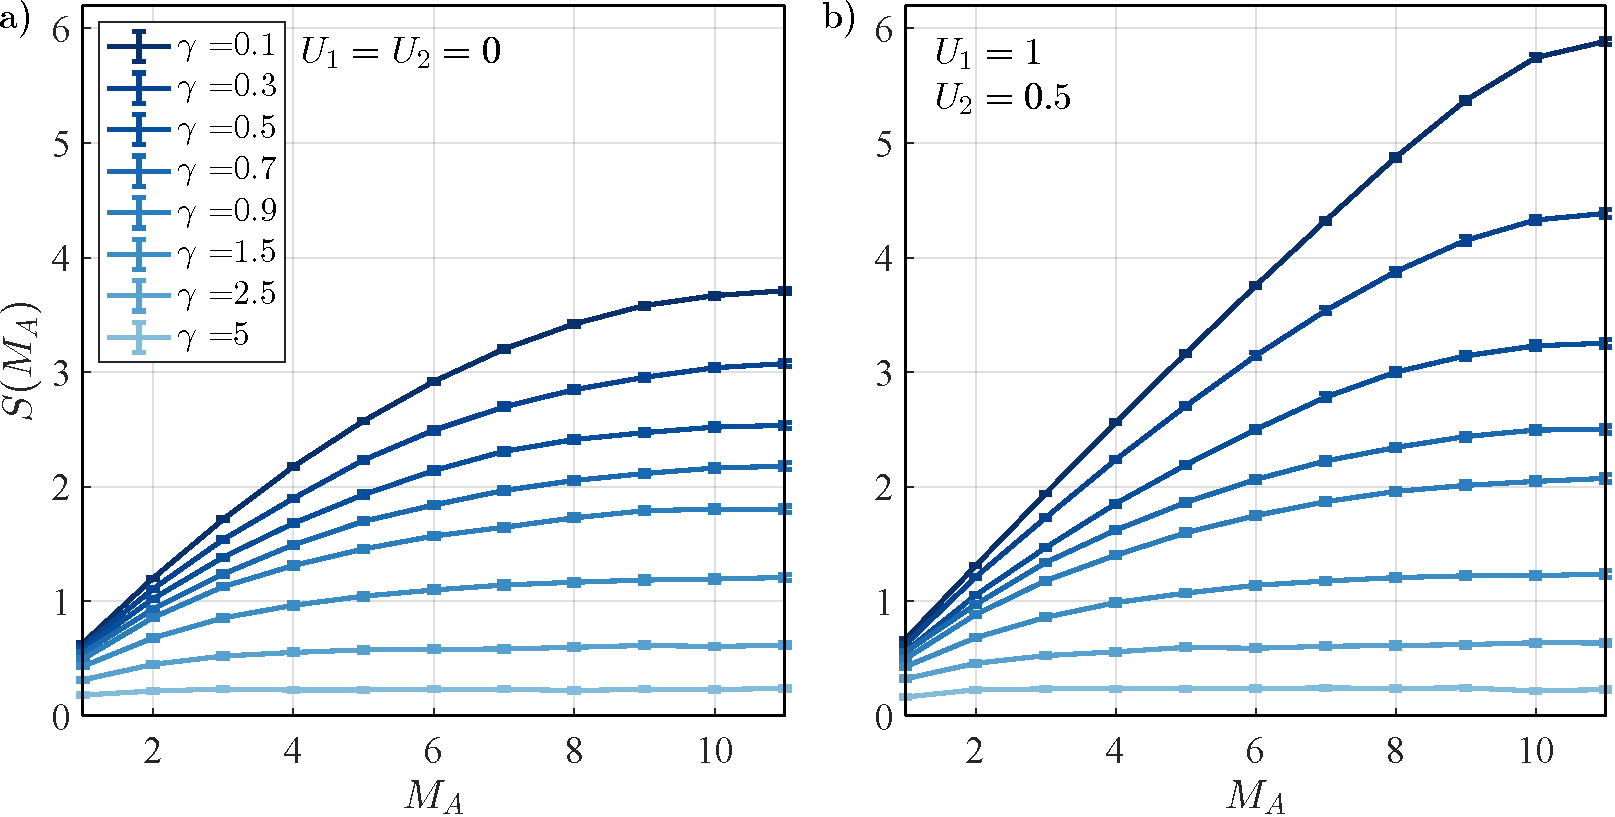
\includegraphics[width=\textwidth]{Chapters/Plots/Chapter4/Chapter3_Fig2.pdf}
        \caption{The von Neumann entropy $S(M_A)$ of the approximate stationary state as a function of subsystem size $M_A$ ($M=22$) for a) the non-interacting model $U_1 = U_2 = 0$, and b) the interacting model with $U_1 = 1, U_2 = 0.5$. A range of dissipation strengths is presented, $\gamma \in [0.1,0.3,0.5,0.7,0.9,1.5,2.5,5]$, visualized in dark to light blue. We time-evolve until ~$TJ = 60$ and compute trajectory averages using $N_t = 300$ trajectories. The statistical error bars are computed using $\sigma = \sigma_S / \sqrt{N_t}$, where $\sigma_S$ is the standard deviation of the data. As both plots highlight, the statistical error bars are small, and we observe good convergence. The legend presented in a) also applies to b).}
        \label{fig:Chapter3_Fig2}
    \end{figure}

In Fig.~\ref{fig:Chapter3_Fig2} b), we can see that the entropy displays significantly qualitatively different behavior for small and large $\gamma$ in the interacting model. For small $\gamma$, we see volume-law scaling, characterized by linear growth of the entropy with subsystem size. In contrast, for large $\gamma$, we see that the entanglement entropy remains invariant under the increase of the subsystem size, suggesting area-law scaling. In the volume-law phase, we see that as $M_A \to M/2$, the linear growth starts to curve, showing some logarithmic corrections to the linear growth, as seen in Ref.~\cite{fuji2020}. Even in these relatively small systems, there appears to be a clear transition between volume-law scaling and area-law scaling of the entropy. In contrast, in Fig.~\ref{fig:Chapter3_Fig2} a), in the non-interacting model for small $\gamma$, the entropy only grows logarithmically, is then fully suppressed in the area-law regime and remains constant as a function of subsystem size. The transition between logarithmic scaling and area-law scaling is present in both models and seems to occur around similar dissipation strengths. To characterize the change between these three distinct behavioral patterns, we can fit a function consisting of a linear, a logarithmic, and a constant term,
\begin{equation}
    f(x) = a x + b \ln{x} + c,
\end{equation}
and investigate how the fitting parameters vary with the dissipation strengths. 

\begin{figure}[ht]
    \centering
    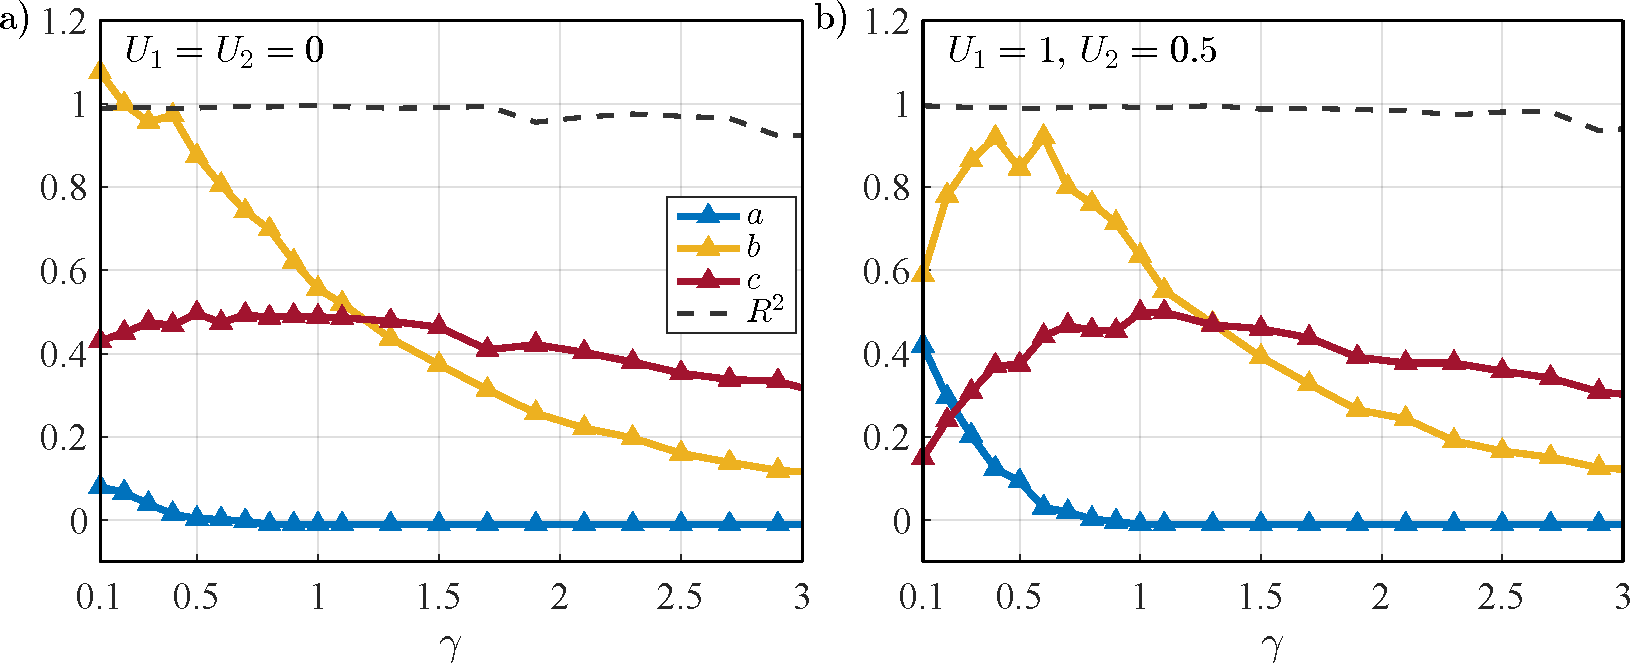
\includegraphics[width=\textwidth]{Chapters/Plots/Chapter4/Chapter3_Fig3.pdf}
    \caption{We plot the coefficients of the fitting function $f(x) = a x + b \ln{x} + c$ as a function of the dissipation strength $\gamma \in [0.1, 3]$ to analyze which terms dominate in which regimes, for a) the non-interacting model and b) the interacting model. The dotted line shows the coefficient of determination $R^2$ close to 1, indicating a good fit for the data. The function $f(x)$ was fitted to the data with $M = 22$ sites to limit the finite-size effects as much as possible. The legend presented in a) also applies to b). Due to the low statistical error bars in Fig.~\ref{fig:Chapter3_Fig2}, we can be confident that the fits we have obtained are accurate. All system parameters are identical to the ones presented in Fig.~\ref{fig:Chapter3_Fig2}}
    \label{fig:Chapter3_Fig3}
\end{figure}

From Fig.~\ref{fig:Chapter3_Fig3}, we can guess where the transition points might lie by analyzing where the different coefficients dominate the scaling behavior. Firstly we can see a clear difference in the linear coefficient $a$. It only plays a small role in the non-interacting case, whereas in the interacting model, we can see a larger contribution matching the behavior we have seen for small $\gamma$ in Fig.~\ref{fig:Chapter3_Fig3}. Secondly, the logarithmic coefficient $b$ dominates the scaling of the entropy in the non-interacting model for small $\gamma$. It continuously decreases with increasing dissipation strength, while in the interacting model, it first grows until $a \approx 0$. Then it also decreases continuously with a similar trend as in the non-interacting model. The constant term $c$ fluctuates around $0.5$ in the non-interacting model while it increases until $\gamma = 1$, and then the qualitative behavior of $c$ appears to be the same in both models. We learn from this figure that there seem to be two regimes for the two models, one in which the fitting coefficients behave differently and one where they appear to exhibit the same trends. While $\gamma<1$, we see significant differences in the fitting parameters between the two models, which is what we would expect as the non-interacting model does not have a volume-law phase while the interacting model does. Then as we have already seen in Fig.~\ref{fig:Chapter3_Fig2}, the transition point between logarithmic and area-law scaling seems to occur around the same dissipation strength, which seems to be in the range $\gamma \in [1,2]$, as this is the regime in which $c$ remains approximately constant, while $b$ continuously approaches $0$. Our data suggests that in the interacting model, a transition between volume-law and logarithmic scaling occurs near $\gamma = 1$, while in both models, a transition appears from logarithmic scaling to area-law scaling on the interval $\gamma \in [1,2]$. Furthermore, the scaling forms of the entropy in the interacting case seem to follow a linear trend with logarithmic corrections and a constant term, and as we approach $\gamma = 1$ the linear term vanishes. After that, logarithmic scaling of the entropy with a constant term describes the behavior of the entropy in the interacting and non-interacting cases.

This analysis provides estimates of which regimes of the parameter space to look for a scaling collapse of the data, also referred to as data collapse. This means rather than considering one single system size to find the transition point; we simulate a range of system sizes and \textit{collapse} all of our data onto a single curve to gain insight into the critical parameters of the transition using a standard scaling form which we introduce below. To further investigate this, we plot the von Neumann entropy in Fig.~\ref{fig:Chapter3_Fig4} between two equally sized subsystems $M_A = M/2$ for a variety of system sizes as a function of the dissipation strength $\gamma$.

\begin{figure}[ht]
    \centering
    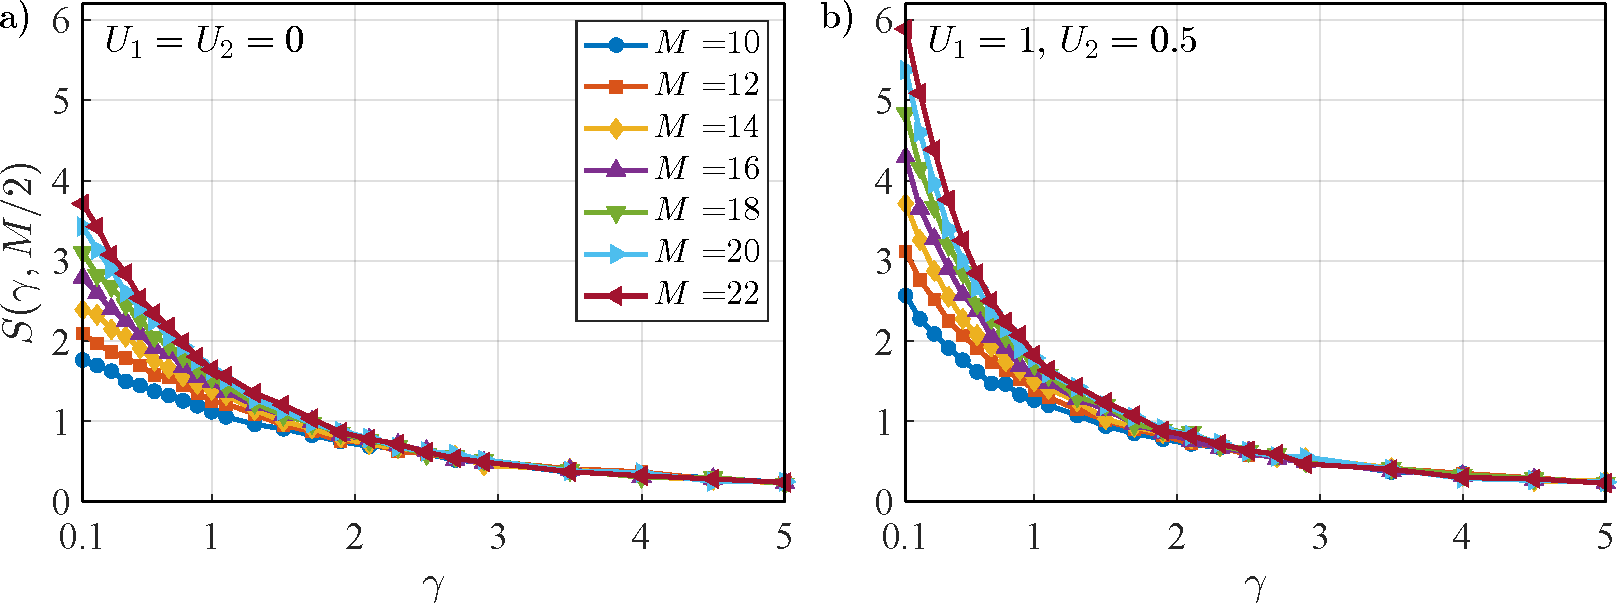
\includegraphics[width=\textwidth]{Chapters/Plots/Chapter4/Chapter3_Fig4.pdf}
    \caption{We plot the trajectory-averaged approximate steady-state von Neumann entropy in the middle bipartition as a function of dissipation strength $\gamma$ for various system sizes. Numerical parameters remain as described in Fig.~\ref{fig:Chapter3_Fig2}. As before, we plot the a) non-interacting case, $U_1 = U_2 = 0$, and b) interacting case $U_1 = 1, U_2 = 0.5$. The legend presented in a) also applies to b).}
    \label{fig:Chapter3_Fig4}
\end{figure}
This plot clearly shows the data begins to collapse in the regime $\gamma \in [1,2]$ for the non-interacting and interacting cases. This is the regime we associate with the transition to area-law scaling; however, this figure reveals no indication regarding a transition from volume-law scaling to logarithmic scaling. Moreover, this figure demonstrates the difficulty of highlighting an exact transition point where the volume-law phase ends, which is most likely due to the limited system sizes we have been able to access in our calculations. We dedicate the next section to the closer examination of this problem by looking at finite size scalings proposed in the literature \cite{skinner2019} and explain the conclusions we draw from our data and calculations.
 
\section{Discussion of scaling collapses}
\label{subsec:discussion_scaling}

In this section, we attempt to pinpoint the critical points at which the transitions between the different regimes occur. As mentioned in the introduction, near criticality, quantum systems are said to be \textit{scale-invariant}. We, therefore, expect that some continuous function describes the behavior of the entropy at criticality, independent of the total system size. In general, we cannot simulate infinitely large systems, which is why we consider a range of accessible system sizes and perform finite size scaling to extract the critical point and exponents. 

From our analysis, we expect the entropy in the vicinity of the critical point to behave as $S(\gamma,M_A) \sim c \ln(M_A)$, where $c$ is a constant. We introduce a scaling function $G(M/\xi)$, where $M$ is the system size and $\xi \sim |\gamma - \gamma_c|^{-\nu}$ describes the correlation length for the critical exponent $\nu$. With this scaling function, we can write, 
\begin{equation}
\label{eq:scalingG}
    S(\gamma,M_A) = c \ln(M_A) + G(M |\gamma - \gamma_c|^{-\nu}).
\end{equation}
By subtracting the entropy at the critical point $S(\gamma_c, M_A)$, we can rewrite Eq.~\ref{eq:scalingG} as,
\begin{equation}
    S(\gamma,M/2) - S(\gamma_c,M/2) = F((\gamma - \gamma_c) M^{1/\nu}), 
\end{equation}
where $F$ is a different scaling function than before, $S(\gamma,M/2)$ is the von Neumann entropy in the steady state between two equal subsystems ($M_A = M/2$) for a dissipation strength $\gamma$ and $\nu$ is the critical exponent associated to the correlation length $\xi \sim |\gamma - \gamma_c|^{-\nu}$.

When $\gamma_c$ and $\nu$ are known, this form can then easily be verified by plotting $S(\gamma,M/2) - S(\gamma_c,M/2)$ as a function of $(\gamma - \gamma_c) M^{1/\nu}$ for a range of system sizes, and all simulated data points should collapse onto a single curve. As in our case, we do not know $\nu$ and have only estimates for $\gamma_c$ we can use this Ansatz to search for the optimal collapse parameters which should pinpoint the transition point. This Ansatz also has been used in related works \cite{skinner2019, fuji2020, li2019} in random circuit models and continuous-time systems.

We now provide a brief overview of the algorithm used to search for the optimal collapse parameters; the full outline is provided in Ref.\cite{skinner2019}. First we define the parameters, $x = (\gamma - \gamma_c) M^{1/\nu}$ and $y(x) = S(\gamma,M/2) - S(\gamma_c,M/2)$. Using spline interpolation for all simulated system sizes, we estimate $S(\gamma_c,M/2)$ for a given estimate $\gamma_c$. We then compute $x$ and $y(x)$ for all simulated parameters $\gamma$ and $M$ in the dataset. This results in a family of curves, and we obtain the optimal scaling parameters by minimizing the mean-square deviation from their mains for any given point $x_i$. All points $x_i$ that lie outside the range of simulated values for $x$ are discarded.

The application of this algorithm to our data has shown scaling collapses for multiple parameter combinations. We expect to see a data collapse at the critical point where we change from one regime into the other. Only the interacting model exhibits a volume-law phase, and from Fig.~\ref{fig:Chapter3_Fig3}~b), we expect that the transition occurs close to where the linear term of the fitting function vanishes, which is the case around $\gamma_c \approx 1$. 

\begin{figure}[ht]
    \centering
    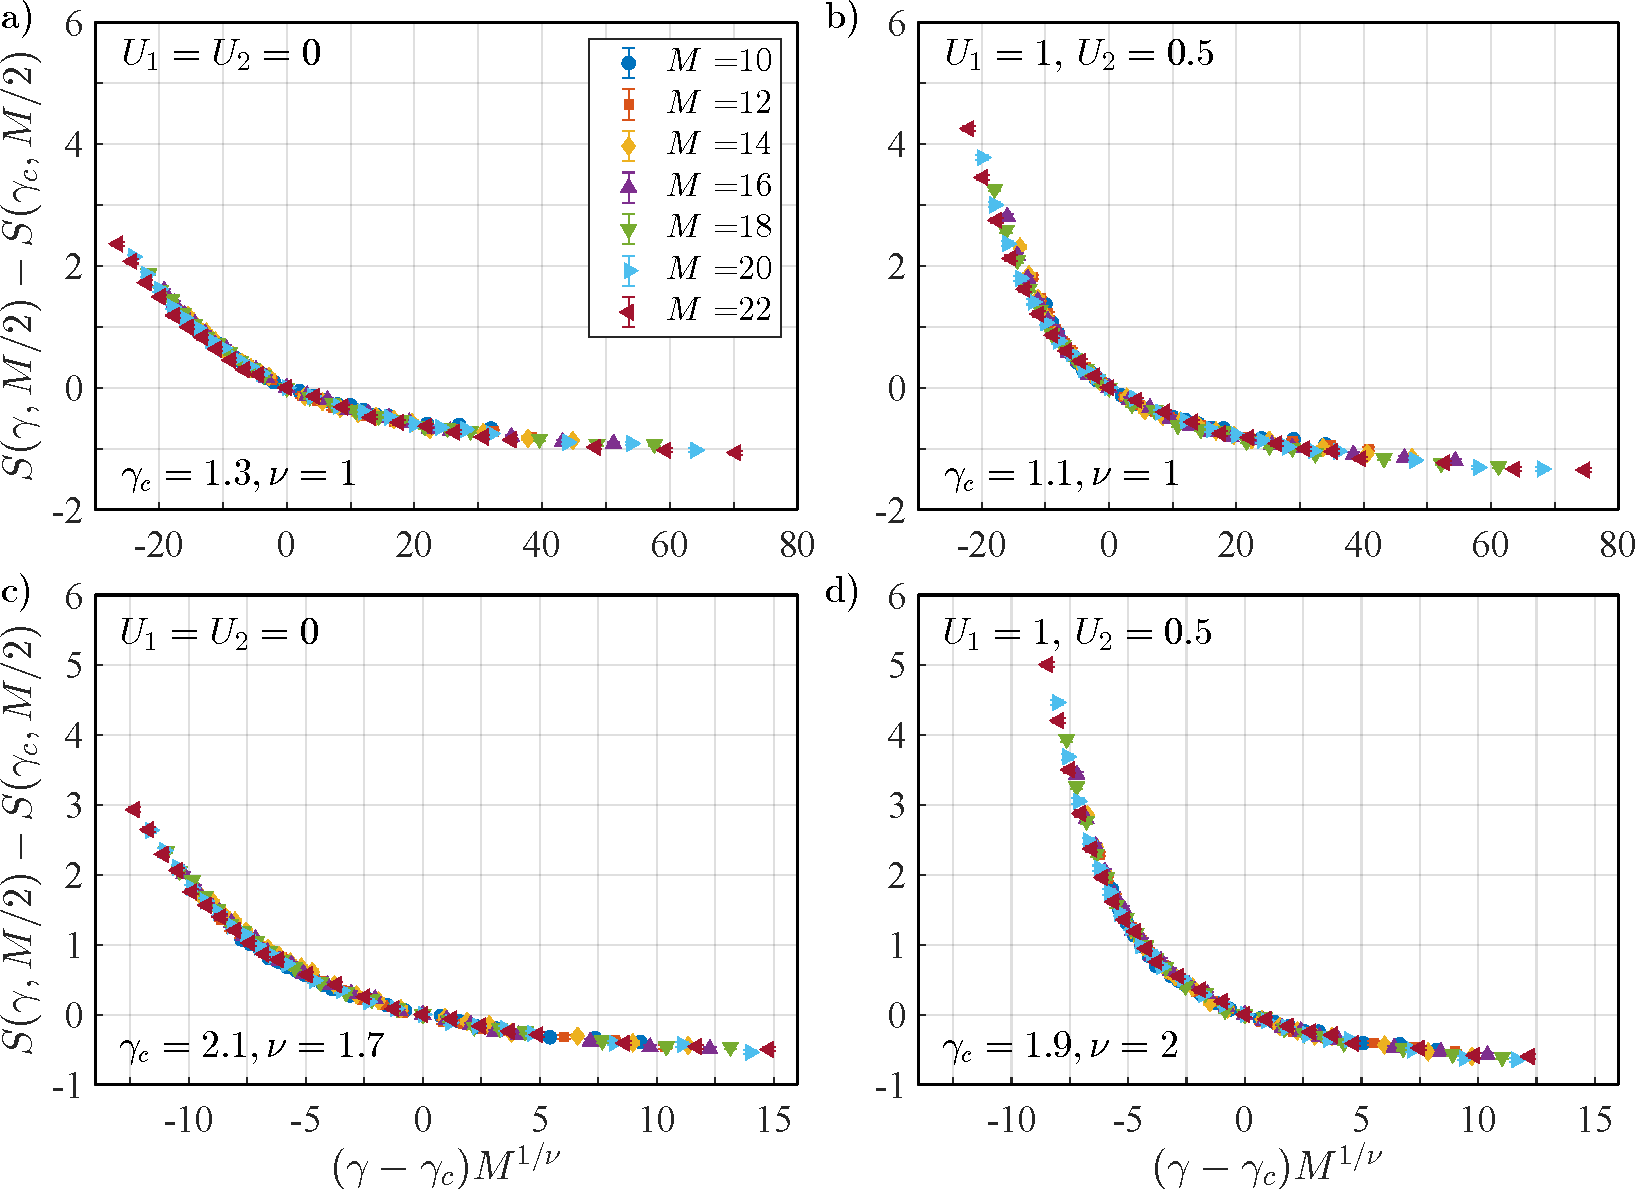
\includegraphics[width=\textwidth]{Chapters/Plots/Chapter4/Chapter3_Fig5.pdf}
    \caption{Scaling collapse of the data from Fig.~\ref{fig:Chapter3_Fig4}, for a) the non-interacting integrable model, and b) the interacting non-integrable model. The scaling parameters depicted here are a) $\gamma_c = 1.3, \nu = 1$, b) $\gamma_c = 1.1, \nu = 1$, c) $\gamma_c = 2.1, \nu = 1.7$, and d) $\gamma_c = 1.9, \nu = 2$. The legend presented in a) also applies to b)-d).}
    \label{fig:Chapter3_Fig5}
\end{figure}

In Fig.~\ref{fig:Chapter3_Fig5}~a)-b) we plot the data collapse in a) the non-interacting model with critical dissipation rate $\gamma_c = 1.3$, and b) in the interacting model with critical dissipation rate $\gamma_c = 1.1$ and $\nu = 1$ in both models. These parameters are obtained by minimizing a cost function, and the resulting scaling collapses are presented here. The critical dissipation rates we have obtained here match our estimates $\gamma \approx 1$, for the volume-law transition. In the non-interacting model, we also see a data collapse for a similar dissipation rate. This is surprising as we do not expect this to happen as this model does not exhibit a volume-law phase. Other parameter values for which the cost function of the search algorithm is minimal could be found, which we have displayed in Fig.~\ref{fig:Chapter3_Fig5}~c)-d). These parameter values match our estimates, where we expect the transition from logarithmic to area-law scaling for $\gamma \approx 2$. As this behavior is present in both models here, we would expect to see a data collapse in both models. 

Furthermore, we found that it was possible to obtain collapses for other parameter values in the non-interacting model. This means that although we observe the transition in the entanglement entropy, we are not able to pinpoint the critical dissipation rates exactly, as we are able to collapse the data for a variety of parameter values, suggesting that the system sizes that we have explored here are not large enough. 

To test whether the system size is the issue, we use Fermionic Gaussian States (FGS) and consider a 1D-chain of free fermions. The non-interacting model we have considered is described by a quadratic Hamiltonian, which allows us to efficiently simulate larger systems consisting of free fermions using the methods introduced in chapter~\ref{sec:FGS}. We simulate the same system sizes that we explored for the hard-core bosons, perform a data collapse, and then add larger system sizes to see whether the data collapse remains unchanged. 

\begin{figure}[ht]
    \centering
    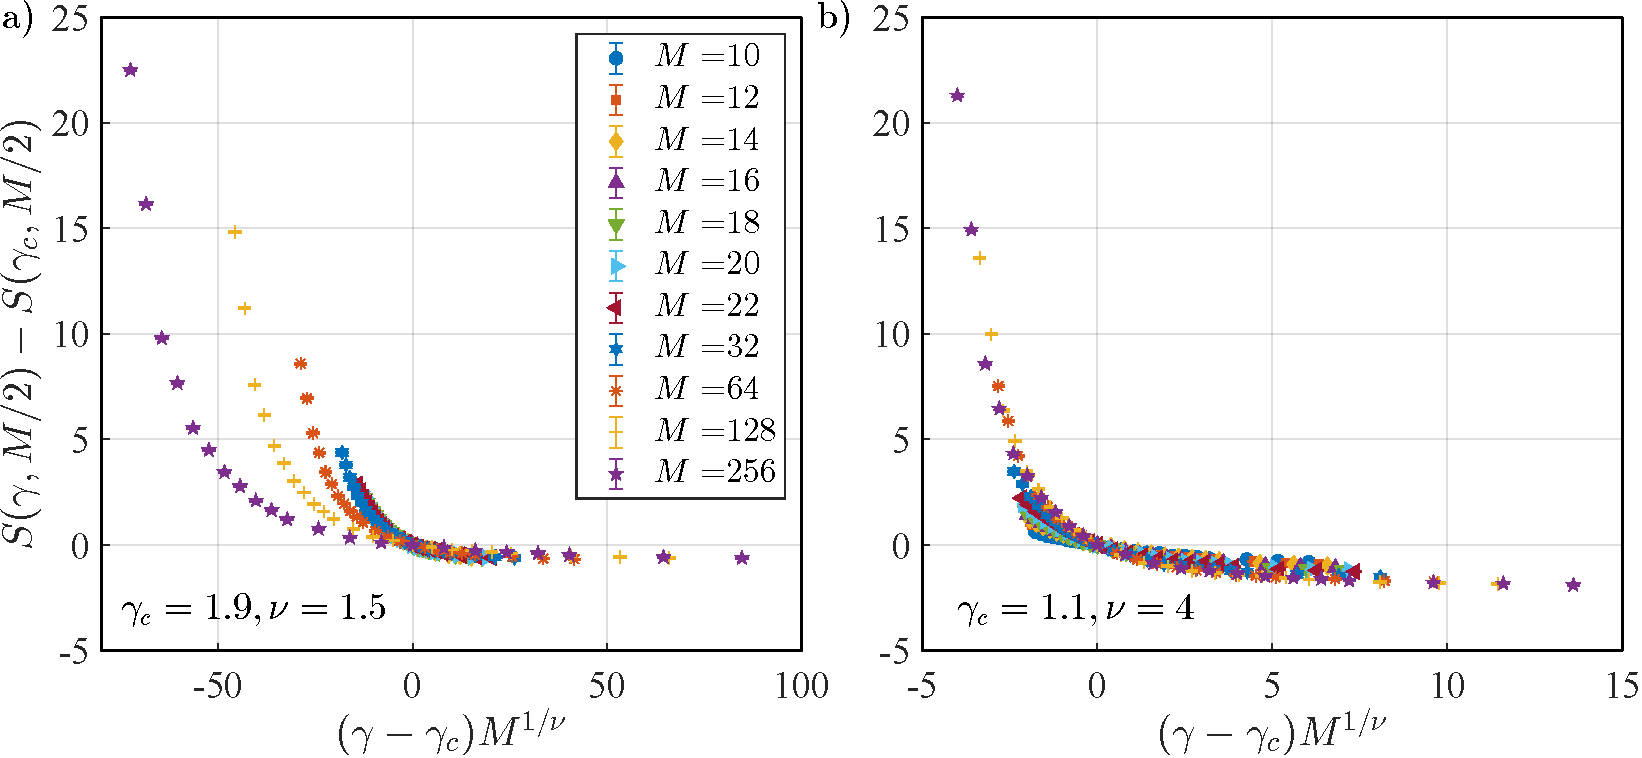
\includegraphics[width=\textwidth]{Chapters/Plots/Chapter4/Chapter3_Fig6.pdf}
    \caption{Scaling collapse of the von Neumann entropy in the fermionic system. In a), we use system sizes $M \leq 32$ to search for optimal collapse parameters; in b), we use the system sizes $M \geq 64$. We then plot the resulting data collapse for all the parameters. The depicted scaling parameters are a) $\gamma_c = 1.9, \nu = 1.5$, and b) $\gamma_c = 1.1, \nu = 4$. The legend presented in a) also applies to b).}
    \label{fig:Chapter3_Fig6}
\end{figure}

Fig.~\ref{fig:Chapter3_Fig6}~a) shows the data collapse when we only include system sizes $M \leq 32$ in the data set. We find that $\gamma_c = 1.9, \nu = 1.5$ leads to the optimal data collapse. This plot clearly shows, however, that the scaling collapse does not work for larger system sizes, which means the system sizes in the data set are simply too small. Furthermore, if we use the large system sizes and perform a data collapse, depicted in Fig.~\ref{fig:Chapter3_Fig6}~b), we see a much better data collapse, where the smaller system sizes follow the trend of the larger ones. 

In this section, we have demonstrated that we can clearly distinguish the different regimes by plotting the entropy as a function of system size; however, we cannot make definitive claims about where the transition points lie when we can only access relatively small system sizes. We have observed large deviations in the scaling collapses when including and excluding certain system sizes for the free fermion model. Moreover, for the hard-core boson data, we expect a data collapse for the interacting model at small measurement strengths but do not expect one in the non-interacting model. Fig.~\ref{fig:Chapter3_Fig5}~a), b), however, shows data collapses for similar collapse parameters in the interacting and non-interacting model, irrespective of whether or not we expect a data collapse to occur. We conclude that we cannot trust the data collapses and critical parameters we extract from a data set if it only contains data for small system sizes.

\section{Breaking the \texorpdfstring{$U(1)$}~~symmetry: single pump and loss}

In this section, we will focus on Model II as described in section~\ref{subsec:model2}. Instead of considering a local dephasing process, we introduce single-particle pump and loss in the system. In Model I, we conserve the $U(1)$ symmetry associated with the total particle number conservation. By considering single pump and loss processes, with respective strengths, $\gamma^+$, and $\gamma^-$, we explicitly break the particle number conservation to explore whether we can witness and pinpoint the transition. For the remainder of this section, we will only consider the case $\gamma^\pm = \gamma^+ = \gamma^-$ to ensure the steady state remains the infinite temperature state with average particle number $M/2$. 

\begin{figure}[hbt!]
    \centering
    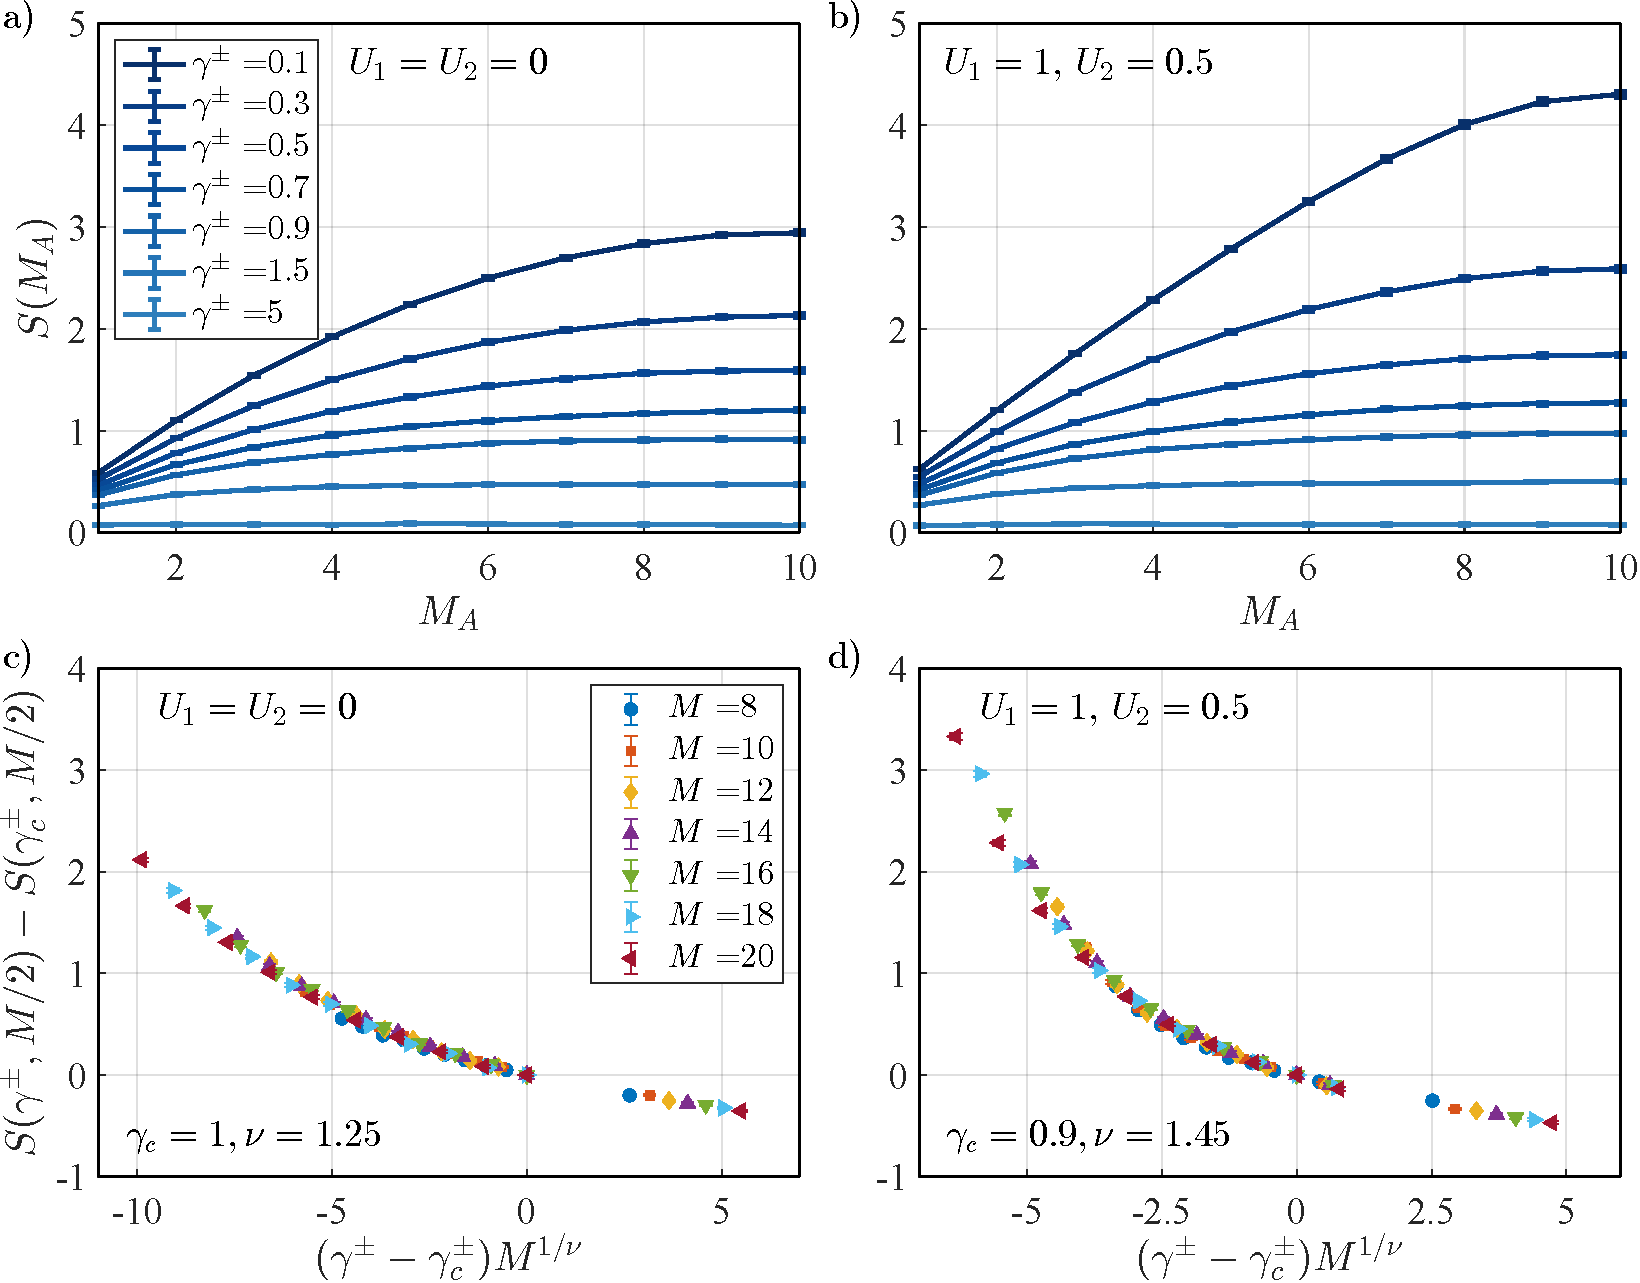
\includegraphics[width=0.99\textwidth]{Chapters/Plots/Chapter4/Chapter3_Fig7.pdf}
    \caption{a)-b) The von Neumann entropy of the approximate stationary state as a function of subsystem size $M_A$ ($M=20$) for a) the non-interacting model $U_1 = U_2 = 0$, and b) the interacting model with $U_1 = 1, U_2 = 0.5$. We time-evolve until $TJ = 60$ and compute trajectory averages using $N_t = 300$ trajectories. The legend presented in a) also applies to b). c)-d) Scaling collapse of the data from a)-b) for the non-interacting and interacting models, respectively. The statistical error bars for a) and b) were calculated in the same fashion as in Fig.~\ref{fig:Chapter3_Fig2} and are sufficiently small, indicating good convergence. The scaling parameters depicted here are c) $\gamma^\pm_c = 1, \nu = 1.25$, and d) $\gamma^\pm_c = 0.9, \nu = 1.45$.}
    \label{fig:Chapter3_Fig7}
\end{figure}

In Fig.~\ref{fig:Chapter3_Fig7}~a)-b), we plot the von Neumann entropy for the non-interacting and interacting models, respectively. As before, we witness volume-law scaling of the entropy in the interacting model for small dissipation strengths $\gamma^\pm$, characterized by linear growth of the entropy with subsystem size. Moreover, as for Model I, we witness a logarithmic regime, which then transitions into an area-law phase where the entropy is constant. We see that there are no qualitative differences in the behavior of the entropy when compared to the case of dephasing despite explicitly breaking the $U(1)$ symmetry. Although we clearly see different signatures in the behavior of the entropy, it is difficult to pinpoint the exact transition point. In Fig~\ref{fig:Chapter3_Fig7}~c)-d), we plot the scaling collapses of the von Neumann entropy of the bipartition, $M_A = [1, M/2]$, for the optimal scaling parameters. Again, we see a similar situation as before: similar critical dissipation strength and exponents collapse the data. In addition, we found other parameters that also collapsed the data, further proving that the accessible system sizes were not sufficiently large to pinpoint the critical point exactly. 

\section{Conclusion}

In this chapter, we have explored the dynamical phase transition that arises due to the competition between coherent time evolution and disentangling dissipative processes such as dephasing and single particle pump and loss. We have seen that we can clearly distinguish between different regimes characterized by the behavior of the entanglement entropy. When using standard methods to extract critical parameters to reveal the transition points, we find that scaling collapses can appear regardless of whether a transition occurs. We have seen that for similar critical parameters, we see data collapses in the bosonic system in both the interacting and non-interacting models, which is concerning since we do not see a transition from volume-law to logarithmic scaling of the entropy in the non-interacting model. We are limited to moderate system sizes ($M \sim 20$) that we can simulate using exact diagonalization, and we do not have the same tools as in random circuits where efficient algorithms exist for system sizes that are an order of magnitude larger ($M \sim 10^2$). 

For the non-interacting model, we also considered a system of free fermions, where we simulated the same system sizes as for the bosonic system but also included larger system sizes, up to $M = 256$. This allowed us to assess the quality of the data collapse we witnessed in the bosonic system by considering different subsets of the system sizes. We first only used small system sizes to obtain a data collapse, which drastically changed upon including the large system sizes to extract the collapse parameters. Furthermore, the collapse parameters we extracted using only the small system sizes do not collapse the larger ones. We, therefore, conclude from this analysis that it is difficult to pinpoint the transition point precisely when we only have access to small system sizes, and we cannot necessarily trust the collapse results when only considering small system sizes, as we did in the bosonic case.

We further explored a system consisting of hard-core bosons, described by the same Hamiltonian but with a single particle pump and loss term, and found qualitatively the same behavior in the entanglement entropy and distinct regimes. Similarly, as for the first model, we see again that scaling collapses appear whether or not a transition occurs, resulting in the conclusion that the accessible system sizes we have been able to explore are too small to make exact claims regarding the precise location of the critical points at which the transitions occur. 

A natural approach to simulate larger system sizes would be to write the system wave function as a matrix product state, which could efficiently represent the state in the area-law regime. In the volume-law regime, however, we could not efficiently represent the system wave function as the truncation to low bond dimensions in the matrix product state relies on working with states that only have moderate or small amounts of entanglement. This clearly is not the case in the volume-law regime, making this not a suitable solution for this problem. 

In the following chapters, we will continue to explore the competition between unitary and dissipative dynamics that give rise to MIPTs. We explore questions regarding the experimental detection of such dynamical phase transitions in chapter~\ref{chap:MIPT_continuous_measurement} and our efforts to find observables that witness the transition that would be experimentally feasible. In chapter~\ref{chap:short_time_dynamics}, we explore whether we can find evidence of different regimes when considering the short-time dynamics as we have only explored the behavior of the stationary states. We further explore whether we can find a feasible method of revealing the transition in an experiment. 

	
	\chapter{Nonlinear Correlations and Measurement-Induced Phase Transitions}
\thispagestyle{empty}
\label{chap:MIPT_continuous_measurement}

In this chapter, we present a project which evolved from the work presented in the previous chapter. We saw that we can model free fermions for larger system sizes, and this makes it natural to explore ways to experimentally detect the measurement-induced phase transition discovered by Alberton et al.~\cite{alberton2021}. We show that a correlation function, which we introduce below, is able to distinguish between the two phases that emerge when changing the measurement strength. Moreover, we are able to reconstruct this correlation function from linear information extracted from many measurement trajectories. This initially suggests that it might be possible to extract the behavior of the correlation function from the noisy measurement record, which emerges naturally from our measurement scheme. However, what can be measured is very subtle, and we found that this cannot be directly measured in experiments. In this chapter, we present the work we did in this project and also show why it is not possible to extract any nonlinear information from different measurement outcomes.

\section{Introduction}

In chapter~\ref{chap:MIPT_bosons}, we explored a system consisting of hardcore bosons where coherent dynamics compete with projective measurements, leading to measurement-induced phase transitions. We simulated the non-interacting case for free fermions as it allowed us to access larger system sizes and helped in our analysis of the bosonic system. In this chapter, however, we will exclusively consider free fermions and explore whether we can detect the transition resulting from the competition between coherent Hamiltonian dynamics and continuous local weak measurement~\cite{szyniszewski2019,romito2020}, illustrated in Fig.~\ref{fig:Chapter4_Fig1}a). In this model, the system undergoes a MIPT from a critical to an area-law regime~\cite{alberton2021}, with a schematic representation of the phase diagram in Fig.~\ref{fig:Chapter4_Fig1}b).

    \begin{figure}[ht]
        \centering
        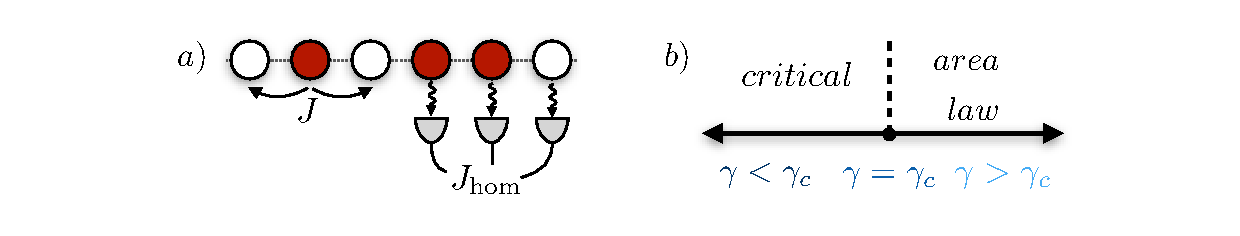
\includegraphics[width = \textwidth]{Chapters/Plots/Chapter5/Chapter4_Fig1.pdf}
        \caption{a) Schematic representation of free fermions on a 1D chain with nearest-neighbor hoping and subject to continuous measurement of the local particle number. b) Schematic representation of the phase diagram as a function of the measurement strength $\gamma$.}
        \label{fig:Chapter4_Fig1}
    \end{figure}
    
As we saw in chapter~\ref{chap:MIPT_bosons}, these phases are characterized by a logarithmic scaling of the entanglement entropy in the critical regime and constant entanglement entropy with subsystem size in the area-law regime. Furthermore, we will show that we can distinguish between the two phases using a nonlinear correlation function, which decays algebraically in the critical regime and exponentially in the area-law regime. Although both quantities are extremely useful in characterizing and distinguishing different phases, they cannot be measured efficiently in experiments, as this would require reproducing individual stochastic trajectories more than once. As in previous sections, the MIPT is not present at the level of the density operator as the trajectory-averaged density matrix is the trivial infinite temperature state for any non-zero measurement rate \cite{li2018,li2019,bao2020,alberton2021}, from which we cannot extract any useful information. Nonlinear functions of the state, however, capture information on the competition between the coherent Hamiltonian dynamics and the continuous weak measurements. 

Suitable nonlinear functions include the von Neumann entropy (Eq.~\ref{eq:vnE}), which we already used to distinguish different phases in chapter~\ref{chap:MIPT_bosons}. Furthermore, the second moment of the two-point correlation function $C_2(l,m) = \overline{|\langle \hat{a}^\dagger_l \hat{a}_{m} \rangle|^2}$, (where $\hat{a}^\dagger_i,\hat{a}_i$ are fermionic creation and annihilation operators respectively in site $i$ and $\overline{.\phantom{l}.\phantom{l}.}$ denotes trajectory averaging), displays a non-trivial trajectory average, which we present in the next section. Note that $\langle \hat{a}^\dagger_l \hat{a}_{m} \rangle$ is non-hermitian. However, we consider the second moment of the correlation function and we will see that this quantity can also be expressed as the connected-correlation function between the local fermion densities $\hat{n}_l$ and $\hat{n}_{m}$ (with $\hat{n}_i = \hat{a}_i^\dagger \hat{a}_i$). We continue by introducing the model we consider in this chapter, exploring whether it is possible to reconstruct the correlation function using only linear information in the density operator and the difficulties we have encountered when extending this idea to experimental setups.

\section{Free Fermion Chain with Continuous Weak Measurement}

In this chapter, we consider free fermions on a periodic, one-dimensional chain with nearest-neighbor hopping that are subject to continuous measurement of the local particle number, as illustrated in Fig.~\ref{fig:Chapter4_Fig1}a). The quadratic hopping Hamiltonian for a chain consisting of $M$ sites is, 
\begin{equation}
H =-J \sum\limits_{i=1}^{M} ( \hat{a}^{\dagger}_i \hat{a}_{i+1} + \hat{a}_i \hat{a}^{\dagger}_{i+1}),
\end{equation}
where $J$ is the tunneling amplitude, $\hat{a}^{\dagger}_i$,$\hat{a}_i$ are the respective fermionic creation and annihilation operators on site $i$. We also assume periodic boundary conditions to limit finite-size effects seen in our analysis. Coherent dynamics lead to a build-up of entanglement as particles hop between neighboring sites while the continuous measurement of the local fermion densities $\hat{n}_i = \hat{a}_i^\dagger \hat{a}_i$ reduces entanglement. This competition leads to a MIPT from a critical phase to an area-law phase \cite{alberton2021}, as noted above. 

We consider a specific type of continuous weak measurement \cite{wiseman2009,jacobs2006}, namely homodyne detection ~\cite{barchielli1991,gisin1992,wiseman1993}, which we introduced in section~\ref{subsec:hom_detec} and may be realized via dispersive coupling of the fermions to cavity photons~\cite{yang2018} or fluorescence measurements of superconducting qubits~\cite{campagne-ibarcq2016}. Yang et al. propose a scheme where a scanning microscope monitors the quantum dynamics of a system in a cavity QED setup. In this scheme, atoms manifest their presence via resonance shifts in the output field of the cavity, which is mixed with a local oscillator, resulting in a homodyne current containing information about the atomic densities. Campagne-Ibarcq et al. propose a scheme where the fluorescence field of qubits is measured using heterodyne detection, which allows the authors to gain information about the state of the qubits. 

The time evolution of the fermion wavefunction follows the stochastic Schr\"{o}dinger equation (SSE), which we defined in section \ref{subsec:qsd},
\begin{equation}
\label{eq:SSE1}
    \ket{\psi(t+dt} = \Big(1-iH dt + \sum\limits_{i=1}^M\Big[ \sqrt{\gamma} \tilde n_{i,t} dW_{i,t}- \frac{\gamma}{2} \tilde n_{i,t}^2 dt\Big]  \Big) \ket{\psi_t},   
\end{equation}
where $\tilde n_{i,t} = \hat{n}_i - \expectation{\hat{n}_i}_t$ which includes a state dependence, $\gamma$ is the measurement rate, and $dW_{i,t}$ is Wiener increment with mean $0$ and variance $dt$, satisfying the conditions described in Eq.~\ref{eq:noise}.

As we discussed in section~\ref{sec:FGS}, the SSE \ref{eq:SSE1} is quadratic in fermion operators, and the dynamics of the wave function can be simulated efficiently in terms of Fermionic Gaussian States (FGS). In this case, the fermion wave function is completely characterized by the correlation matrix, $D_{ij} = \langle \hat{a}^\dagger_i \hat{a}_j \rangle$. The detailed numerical procedure is outlined in section \ref{sec:FGS}. 

\section{Reconstruction of the correlation function \texorpdfstring{$C_2(l,m)$}{TEXT} using linear information}

As we have already seen, nonlinear functions allow us to gain insight into the different phases. The critical phase is characterized by logarithmic scaling of the entanglement entropy for small measurement rates and algebraic decay of the correlation function $C_2(l,m)$. However, in the strong measurement regime, measurements prevent entanglement and long-range correlations from building up, resulting in area-law entanglement and exponentially decaying correlations. 

\begin{figure}[ht]
    \centering
    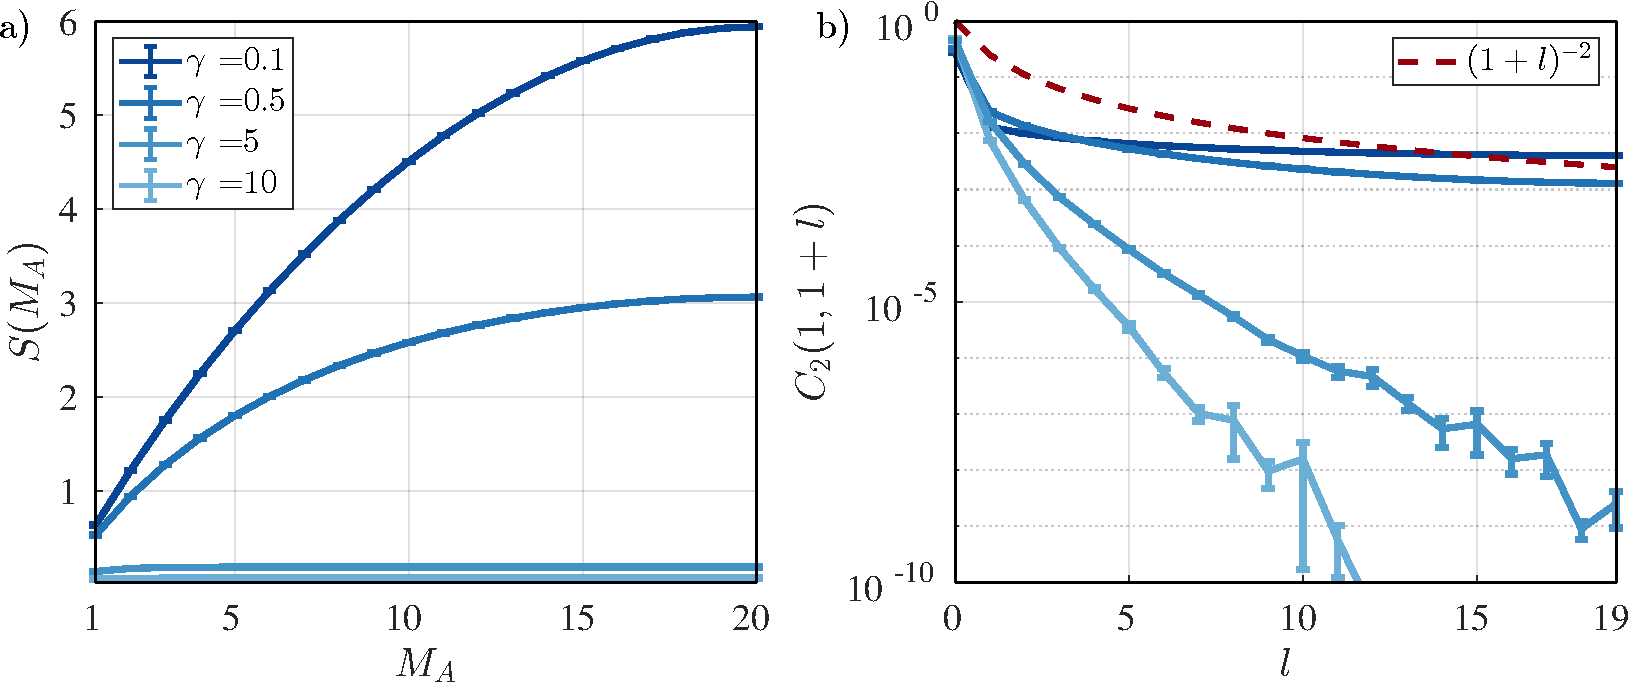
\includegraphics[width=\textwidth]{Chapters/Plots/Chapter5/Chapter4_Fig2.pdf}
    \caption{a) The von Neumann entropy of the approximate stationary state as a function of subsystem $M_A$ ($M = 40$) for measurement strengths, $\gamma = 0.1, 0.5, 5, 10$. b) The correlation function $C_2(1,1+l) = |\expectation{a_1^\dagger a_{1+l}}|^2$ as a function of distance $l$. We time-evolve until $TJ = 60$ and compute trajectory averages using $N_t = 10^6$ trajectories. The legend presented in a) applies also to b).}
    \label{fig:Chapter4_Fig2}
\end{figure}

In Fig.~\ref{fig:Chapter4_Fig2}~a), we plot the von Neumann entropy in the approximate steady state as a function of the subsystem size for a range of measurement strengths. We observe logarithmic scaling of the entropy with the subsystem size for the small measurement strengths. In contrast, in the large measurement regime, the entanglement only grows minimally and afterward remains constant. In Fig.~\ref{fig:Chapter4_Fig2}~b), we plot the correlation function $C_2(1,1+l)$ as a function of the distance $l$, which also witnesses the transition. For small measurement strengths, we observe the correlation function follows the same qualitative behavior as that of the curve $(1+l)^{-2}$, indicating algebraic decay. We also observe the characteristic exponential decay of the correlation function with the distance $l$ for the large measurement strengths, which is indicated here by the linear downward trend on the logarithmic scale.

As noted before, we cannot measure these quantities in an experiment as this would require accessing individual trajectories multiple times. We can, however, express the connected correlation function in terms of number operators \cite{alberton2021}, 
\begin{equation}
    C_2(l,m) = \overline{|\langle \hat{a}^\dagger_l \hat{a}_{m} \rangle|^2} = \overline{\expectation{\hat{n}_l} \expectation{\hat{n}_m}} - \overline{\expectation{\hat{n}_l \hat{n}_m}},
\end{equation}
where $\expectation{n_i}$ are the expectation values of the local number operators in site $i$. The second term in this expression $\overline{\expectation{\hat{n}_l \hat{n}_m}}$ corresponds to the linear average in the infinite temperature state and is determined by the initial state. We consider an initial product state at half filling, and as we time-evolve under a number-conserving Hamiltonian, the total particle number does not change. 
Therefore, if we measure $n_m$ the probability of detecting a particle at site $m$ to not detecting it is $N/M$ on average, and then as we have $N-1$ particles left, spread over $M-1$ sites, the probability of detecting a particle at site $l$ to not detecting it, is $\dfrac{N-1}{M-1}$ on average after measuring $n_m$. Hence we have, 
\begin{equation}
    \overline{\expectation{\hat{n}_l \hat{n}_m}} = \frac{N}{M}\frac{N-1}{M-1},
\end{equation}
where $N = M/2$ as we only consider initial states at half-filling. Note that in the thermodynamic limit, as $M\to\infty$, $\overline{\expectation{\hat{n}_l \hat{n}_m}} \to \frac{1}{4}$. Using this we can reconstruct the correlation function $C_2(l,m)$, 
\begin{equation}
   \tilde C_2(l,m) = \overline{\expectation{\hat{n}_l} \expectation{\hat{n}_m}} - \frac{N}{M}\frac{N-1}{M-1},
\end{equation}
where $\tilde C_2(l,m)$ is the correlation function computed directly from the local fermion densities. 

In Fig.~\ref{fig:Chapter4_Fig3}, we plot $\tilde C_2(i,i+l)$ as a function of the distance $l$, where we have averaged over all sites, as well as over the time interval $TJ \in [55, 60]$, to reduce the statistical errors as much as possible. We also plot $C_2(i,i+l)$ to compare it to the reconstructed correlation function.

\begin{figure}[ht]
    \centering
    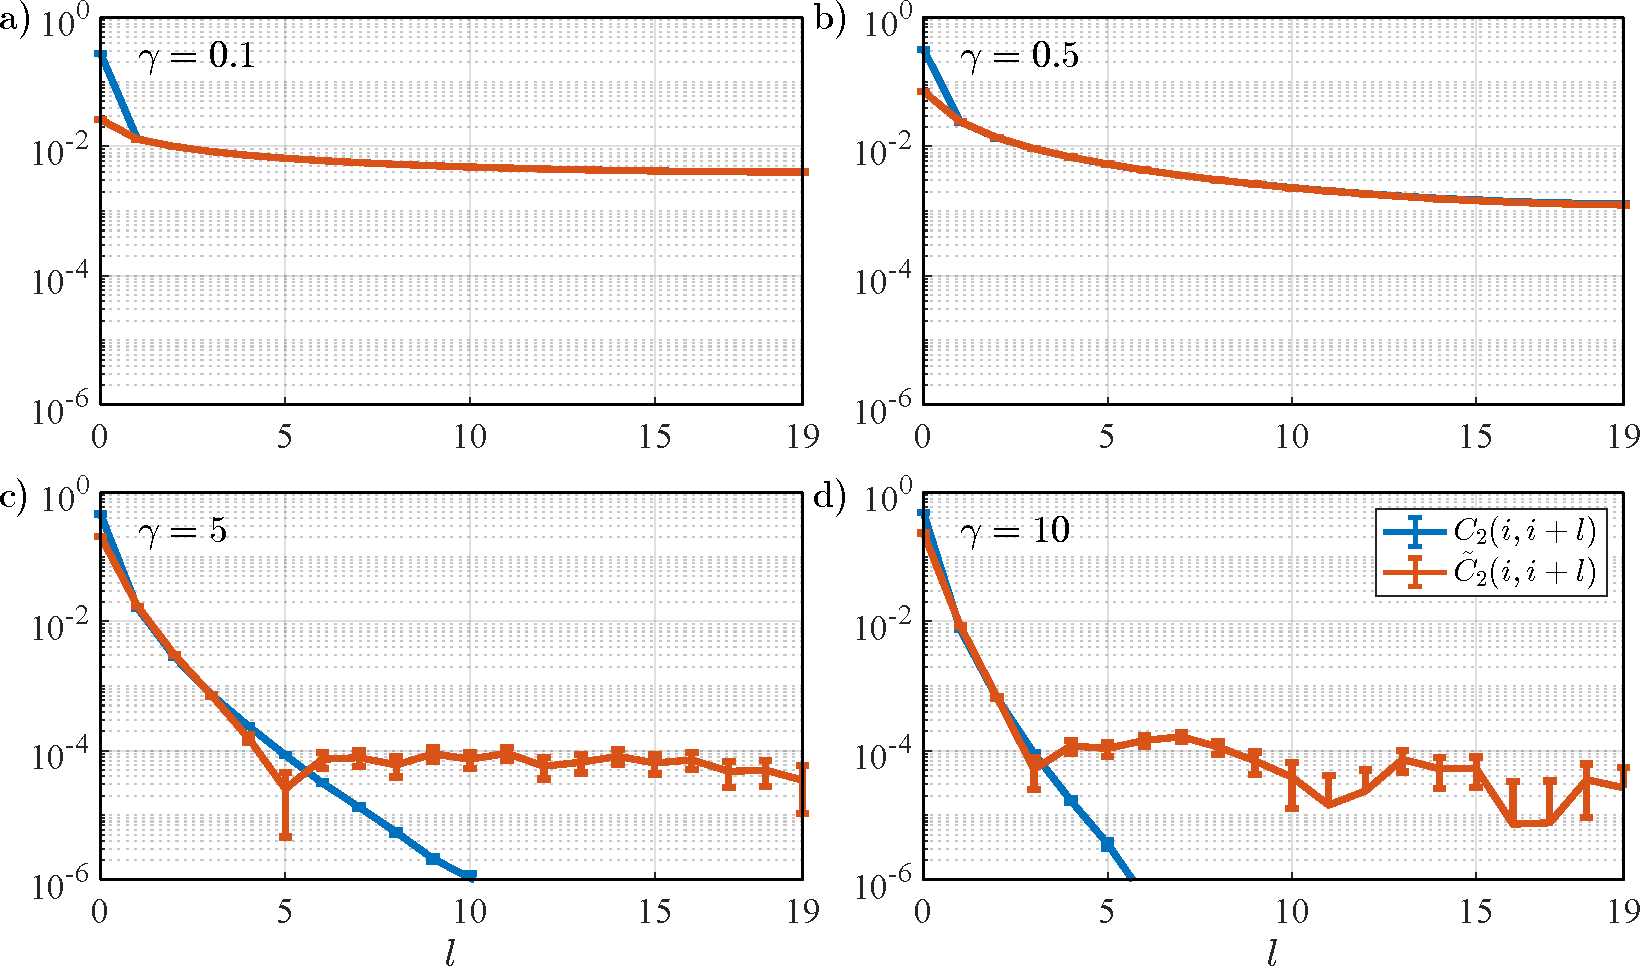
\includegraphics[width=\textwidth]{Chapters/Plots/Chapter5/Chapter4_Fig3.pdf}
    \caption{The second moment of the correlation function $C_2(i,i+l) = |\expectation{a_i^\dagger a_{i+l}}|^2$ as a function of distance $l$. We compare $C_2(i,i+l)$ to $\tilde C_2(i,i+l)$, which is the correlation function computed from the local fermion densities. We time-evolve until $TJ = 60$, with a numerical time step $dt = 0.01$, and compute trajectory averages using $N_t = 10^6$ trajectories. We further average $\tilde C_2(i,i+l)$ over the interval $TJ\in[55,60]$ and spatially average over all sites, $i \in [1,40]$. The legend presented in d) applies also to a)-c).}
    \label{fig:Chapter4_Fig3}
\end{figure}

 In Fig.~\ref{fig:Chapter4_Fig3}~a), b) we plot the correlation functions for $\gamma = 0.1, 0.5$ respectively, and we observe near perfect overlap between the two correlation functions, indicating that this method in the small measurement regime works very well. In the large measurement regime, however, the correlations decay faster than the statistical errors, which we observe in Fig.~\ref{fig:Chapter4_Fig3}~c), d) where we plot the correlation functions for $\gamma = 5, 10$ respectively. We initially see a good agreement to roughly a distance $l \sim 4,5$ between the two correlation functions. At distances $l > 5$, the correlation function computed directly from the state continues to decrease fast, while the reconstructed correlation function remains approximately constant at an order of magnitude $\sim 10^{-4}$. Furthermore, the error bars are roughly of the same order of magnitude, which implies we have reached the maximal accuracy we can achieve with the number of trajectories we have simulated. As the statistical errors scale with $\sqrt{N_t}$, we would need to compute $100$ times as many trajectories, which is not feasible as we already simulate $10^6$ trajectories.

Although we only have an agreement for short distances in the large measurement regime, this shows that it is possible to reconstruct the correlation function using only the local fermion densities, which are linear in the density operator, although it requires a lot of sampling. This is, in principle, an interesting starting point, but (perhaps surprisingly) this correlation function is not accessible in experiments.

\section{Correlations of homodyne currents at different sites}

Given that $C_2(l,m)$ is related to $\expectation{\hat{n}_l} \expectation{\hat{n}_m}$ it is natural to ask if this might be extracted from $\expectation{J_l(t) J_m(t)}$ and we will show here what is obtained. The type of continuous weak measurement we consider results in homodyne currents, 
\begin{equation}
    J_i(t) = \expectation{n_i(t)} + \xi_i(t) 
\end{equation}
which are continuous random variables, with $\xi_i(t) = \dfrac{dW_i(t)}{\sqrt{\gamma} dt}$ as we have discussed. $\xi_i(t)$ is a Wiener process, which by definition has zero mean, and hence by averaging homodyne currents, we can measure the local fermion densities, $\overline{J_i(t)} = \overline{\expectation{n_i(t)}}$. Since this quantity is linear in the density operator, it is useless to us, as the average corresponds to the expectation value in the trivial infinite temperature. 

On the other hand, averaging the product of homodyne currents is nonlinear in the density operator, and we gain access to information about the competition between coherent and dissipative dynamics. Let us consider the average over different noise realizations of the product of two instantaneous homodyne currents (in It\^o calculus) at time $t$,
\begin{align}
\begin{split}
    \overline{J_l(t) J_m(t)} &= \overline{\Big(\expectation{n_l(t)} +  \xi_l(t) \Big) \Big(\expectation{n_m(t)} +  \xi_m(t)  \Big)} \\
     &= \overline{\expectation{n_l(t)}\expectation{n_m(t)}} + \overline{\expectation{n_m(t)}  \xi_l(t)}  + \overline{\expectation{n_l(t)}  \xi_m(t)}  + \overline{\xi_l(t) \xi_m(t)}\\
     &= \overline{\expectation{n_l(t)}\expectation{n_m(t)}},
\end{split}
\end{align}
since for $\overline{\expectation{n_{m,l}(t)}  \xi_{l,m}(t)} = 0$ as they are independent of each other, and by definition, $\overline{\expectation{\xi_l(t)}\expectation{\xi_m(t)}} = 0$ (Eq.~\ref{eq:noise}) for $m \neq l$. 

With this naive approach, limited to a single It\^o step \cite{wiseman1993,wiseman1994, wiseman1994a}, we obtain the desired nonlinear correlations, which allows us to reconstruct the correlation function that witnesses the phase transition. This approach, however, does not reflect an experiment, as the measured homodyne currents are not instantaneous values as we have assumed here but are time-integrated signals. The correct approach is to consider the product of homodyne currents that have been averaged in time before being trajectory-averaged to reflect a realistic measurement signal (or work in a Stratonovich form from the outset). Due to time-averaging, the homodyne signals are now correlated as continuous measurements condition the system, and the wavefunction describing the state at later times depends on the expectation values and noise realizations at earlier times. This means that the products of the type $\expectation{n_{i}(t+dt)}  \xi_{j}(t) $ do not automatically average to zero but instead result in a rather spectacular cancellation of the nonlinear terms that we are interested in measuring. We will now prove why this is the case.

\textbf{Proof}
For the simplest case, let us consider a homodyne current that is averaged over two time steps, 
\begin{align}
\begin{split}
    J_i^\text{avg}  &= \frac{1}{2} \big[ J_i(t)+J_i(t+\delta t) \big] \\ 
                    &= \frac{1}{2} \big[ \expectation{n_i(t)} + \xi_i(t) + \expectation{n_i(t+\delta t)} + \xi_i(t+\delta t) \big]\\
                    &= \frac{1}{2} \big[ \expectation{n_i^0} + \xi_i^0 + \expectation{n_i^1} + \xi_i^1 \big],
\end{split}
\end{align}
where we have introduced the superscripts $0, 1$ for more concise notation. The superscripts denote the time-dependence, $A^0 \equiv A(t)$ and $A^1 \equiv A(t+\delta t)$.

Note that at this point, we still obtain the correct linear expectation values upon averaging, $\overline{J_i^\text{avg}} = \frac{1}{2} (\overline{\expectation{n_i^0}} + \overline{\expectation{n_i^0}})$ as the noise terms have zero mean. Time-averaging the homodyne currents results in the time-averaged expectation values of the fermion densities. The problem leading to the cancellation arises due to the product we compute before trajectory averaging.

Let us consider the product of two homodyne currents that have been averaged over two time steps, 
\begin{align}
\begin{split}
\label{eq:prodJ_expand}
    J_l^\text{avg} J_m^\text{avg} &= \frac{1}{2} \big[ \expectation{n_l^0} + \xi_l^0 + \expectation{n_l^1} + \xi_l^1 \big] \frac{1}{2} \big[ \expectation{n_m^0} + \xi_m^0 + \expectation{n_m^1} + \xi_m^1 \big] \\
    &= \frac{1}{4} \big[ \expectation{n_l^0} + \expectation{n_l^1} \big] \big[ \expectation{n_m^0} + \expectation{n_m^1} \big] + \frac{1}{4} \big[ \xi_l^0 + \xi_l^1 \big] \big[ \xi_m^0 + \xi_m^1 \big] \\
    &+ \frac{1}{4} \big[\expectation{n_l^0} \xi_m^0 + \expectation{n_l^0} \xi_m^1 + \expectation{n_l^1} \xi_m^0 + \expectation{n_l^1} \xi_m^1  \big] \\
    &+ \frac{1}{4} \big[\expectation{n_m^0} \xi_l^0 + \expectation{n_m^0} \xi_l^1 + \expectation{n_m^1} \xi_l^0 + \expectation{n_m^1} \xi_l^1  \big].
\end{split}
\end{align}
This expression looks quite tedious to evaluate; however, if we consider the linear trajectory average of this product, most of these terms will vanish.

First, we have, 
\begin{align}   
    \frac{1}{4} \overline {\big[ \expectation{n_l^0} + \expectation{n_l^1} \big] \big[ \expectation{n_m^0} + \expectation{n_m^1} \big]} = \overline{\expectation{n_l^0} \expectation{n_m^0} },
\end{align}
assuming that in the steady state, the expectation value of the local density does not change considerably, $(\expectation{n_{l,m}^0} + \expectation{n_{l,m}^1})/2 \approx \expectation{n_{l,m}^0}$.

Secondly, 
\begin{align}
    \frac{1}{4} \overline{\big[ \xi_l^0 + \xi_l^1 \big] \big[ \xi_m^0 + \xi_m^1 \big]} = \frac{1}{4} \big[ \overline{\xi_l^0 \xi_m^0} + \overline{\xi_l^0 \xi_m^1} + \overline{\xi_l^1 \xi_m^0} + \overline{\xi_l^1 \xi_m^0 } \big] = 0,
\end{align}
since all noise terms are uncorrelated in time and space and satisfy Eq.~\ref{eq:noise}.

Finally, if we consider the remaining terms in Eq.~\ref{eq:prodJ_expand}, $\overline{\expectation{n_l^0} \xi_m^0} = 0$, $\overline{\expectation{n_l^1} \xi_m^1} = 0$ since these products are uncorrelated at equal times and $\overline{ \expectation{n_l^0} \xi_m^1 } = 0$ as the expectation value is not correlated with the noise term at a later time. Similarly, $\overline{\expectation{n_m^0} \xi_l^0} = 0$, $\overline{\expectation{n_m^1} \xi_l^1} = 0$, and $\overline{ \expectation{n_m^0} \xi_l^1 } = 0$ using the same arguments. The only non-zero terms are $\overline{ \expectation{n_l^1} \xi_m^0}$ and $\overline{ \expectation{n_m^1} \xi_l^0}$, as the conditioned state (and therefore the expectation value) at time $t+\delta t$ depends on the noise at time $t$. 
Removing all the vanishing terms yields, 
\begin{equation}
\label{eq:J_prod}
    \overline{J_l^\text{avg} J_m^\text{avg}} = \overline{\expectation{n_l^0} \expectation{n_m^0} } + \frac{1}{4} \big[\overline{\expectation{n_l^1} \xi_m^0} + \overline{ \expectation{n_m^1} \xi_l^0 } \big].
\end{equation}
To evaluate Eq.~\ref{eq:J_prod}, we need to compute the two non-vanishing terms, and we can do this by using Eq.~4.97 from Wiseman and Milburn~\cite{wiseman2009}, which provides an expression of the conditioned state $\hat{\rho}^1$ at time $t+\delta t$, which reads, 
\begin{equation}
\label{eq:cond}
    \hat{\rho}^1 = \hat{\rho}^0 + \sqrt{\gamma} \sum\limits_i dW_i^0 \big( \{n_i, \hat{\rho}^0\} - 2 \expectation{n_i^0} \hat{\rho}^0 \big),
\end{equation}
where $\{n_i, \hat{\rho}^0\} = n_i \hat{\rho}^0 + \hat{\rho}^0 n_i$ is the anti-commutator.

Then by rewriting $\expectation{n_l^1} = \Tr(\hat{\rho}^1 n_l)$, we can now substitute $\hat{\rho}^1$ from Eq.~\ref{eq:cond},
\begin{align}
\begin{split}
    \overline{\expectation{n_l^1} \xi_m^0} &= \overline{ \Tr(\hat{\rho}^1 n_l) \xi_m^0} \\ 
    &= \overline{ \Tr\Big( \Big[ \hat{\rho}^0 + \sqrt{\gamma} \sum\limits_i dW_i^0 \big( \{n_i, \hat{\rho}^0\} - 2 \expectation{n_i^0} \hat{\rho}^0 \big) \Big]  n_l \Big) \xi_m^0} \\
    &= \overline{\Tr\big( \hat{\rho}^0 n_l \xi_m^0 \big)} + \overline{\Tr\Big( \sum\limits_i dW_i^0 \frac{dW_m^0 }{dt} \big[ \{n_i, \hat{\rho}^0\} - 2 \expectation{n_i^0}\hat{\rho}^0 \big]   n_l \Big)},    
\end{split}
\end{align}

where $\overline{\Tr\big( \hat{\rho}^0 n_l \xi_m^0 \big)} = \overline{\expectation{n_l^0} \xi_m^0} = 0$ as these are uncorrelated, and using $\overline{dW_i^0 dW_m^0} = \delta_{i, m} dt$ we can write,
\begin{align}
\begin{split}
\label{eq:final1}
    \overline{\expectation{n_l^1} \xi_m^0} &= \overline{\Tr\Big( \big[ \{n_m, \hat{\rho}^0\} - 2\expectation{n_m^0} \hat{\rho}^0 \big]   n_l \Big)} \\
    &= \overline{\Tr\Big( \big[ n_m \hat{\rho}^0 + \hat{\rho}^0 n_m \big] n_l \Big)} - \overline{\Tr\Big( 2\expectation{n_m^0} \hat{\rho}^0 n_l \Big)} \\
    &= 2\overline{\expectation{n_l^0 n_m^0}} -2 \overline{\expectation{n_l^0}\expectation{n_m^0}}
\end{split}
\end{align}

Following the same steps, we further obtain, 
\begin{equation}
\label{eq:final2}
    \overline{\expectation{n_m^1} \xi_l^0} = 2\overline{\expectation{n_l^0 n_m^0}} -2 \overline{\expectation{n_l^0}\expectation{n_m^0}}.
\end{equation}
Finally substituting Eq.~\ref{eq:final1}-\ref{eq:final2} in~\ref{eq:J_prod} we obtain, 
\begin{align}
\begin{split}
        \overline{J_l^\text{avg} J_m^\text{avg}} &= \overline{\expectation{n_l^0} \expectation{n_m^0} } + \frac{1}{4} \big[ 4\overline{\expectation{n_l^0 n_m^0}} -4 \overline{\expectation{n_l^0}\expectation{n_m^0}} \big] \\
    &= \overline{\expectation{n_l^0 n_m^0}}. 
\end{split}
\end{align}

$\hfill\blacksquare$

With this, we have proven that we cannot use the product of two time-integrated currents to gain access to nonlinear information of the density operator as this information cancels, and we are only left with the trivial linear average that coincides with the expectation value in the infinite temperature state. 

\section{Discussion}

In this section, we have attempted to find an approach that allows us to access nonlinear information in the density operator, with which one would be able to experimentally witness the measurement-induced phase transition that arises in this model through competition between coherent time evolution and continuous weak measurement of the fermion densities. Due to the weak measurement, a homodyne current arises in which the monitored fermion densities are encoded. This linear information is equivalent to the expectation value in the trivial infinite temperature state, which does not depend on the measurement strength and is, therefore, useless. The second moment of the correlation function witnesses the phase transition, as it exhibits long-ranged algebraically decaying correlations for small measurement strengths and exponentially decaying correlations for large measurement strengths. By rewriting this correlation function in terms of the product of local densities and a linear term, we are, in principle, able to reconstruct the correlation function. As we have seen, this approach requires a large number of trajectories in order to obtain statistical error bars that are small enough, but given access to the local fermion densities, it is possible. The second step of our approach was to consider the product between homodyne currents, hoping to recover the product of fermion densities and, therefore, the correlation function. We realized, however, that this approach was not possible as the homodyne currents are time-integrated correlated signals, which lead to-- cancellations, and we are left with only linear information about the state. This is the reason why this project did not lead to a publication, as we did not manage to find another way in which we would be able to measure the fermion densities. 



	
	\chapter{Probing Competition between Coherent and Dissipative Dynamics At Short Times}
\thispagestyle{empty}
\label{chap:short_time_dynamics}

In this final chapter, we will present a different approach to characterize the competition between coherent dissipative dynamics in the models that we considered in chapter~\ref{chap:MIPT_bosons} and~\ref{chap:MIPT_continuous_measurement}. The content of this chapter is the result of the author's final project, which is presented in Ref.~\cite{bintener2024}.

\section{Introduction}

In the previous two chapters, we have explored the measurement-induced phase transitions that result from the competition between coherent dynamics, which build up entanglement, and quantum correlations and measurements, which lead to the localization of information and a decrease of entanglement. The MIPTs resulting from this competition have been studied in several contexts in recent years~\cite{li2018,li2019,skinner2019} and are characterized by nonlinear functions in the density operator at long times. The time evolution of the system wavefunction follows independent measurement trajectories, where nonlinear functions, upon averaging, display qualitatively different behavior with varying measurement strength. The steady state of the models we have considered is the trivial infinite temperature state, which is reached independently of the measurement strength. Therefore, linear quantities computed from individual trajectories coincide with their expectation values in the infinite temperature state, while nonlinear functions, in general, do not. So far, we have only analyzed the steady-state properties of our models, and two interesting questions arise: Can we relax this requirement, and are we able to distinguish features of the different phases during the short-time dynamics of the system evolution? The transition only clearly is a transition in the steady state as a balance in the competition between coherent and dissipative dynamics has been reached. At short times, we expect that for very small measurement strengths, the behavior of the system is dictated by coherent dynamics. In contrast, at short times, for large measurement strengths, measurements occur so frequently that the system will tend to remain in its initial state. In between, we expect a crossover region rather than the phase transition at a critical measurement strength, as the competition between coherent and dissipative dynamics results in damped oscillations of both linear and non-linear quantities, as we will show in the following sections. Still, relaxing the requirement of only considering steady-state properties allows us to investigate linear functions of the density operator, which, as we will see, can be used to characterize not the phase transition itself but rather the competition between coherent and dissipative dynamics differently than we have seen so far. The goal remains to devise an approach that allows us to find signatures to detect the underlying many-body phenomena experimentally. We conclude this chapter with a reproducible method that allows us to characterize the different behaviors in our model using a cross-trajectory correlator, which we adapt from the protocol from Ref.~\cite{vermersch2019}. We compute the correlator by sampling directly from the infinite temperature state, and we show that although the infinite temperature state itself is featureless, we can discriminate between the area-law and intermediate regime, which is characterized by logarithmic scaling of the von Neumann entropy in the steady state. We now briefly recap the model we have encountered in chapter~\ref{chap:MIPT_bosons} and present the results for early-time dynamics of our model as well as experimental probing of the competition between coherent and dissipative dynamics.

\section{Model}

As mentioned in this chapter, we consider the model we investigated in chapter~\ref{chap:MIPT_bosons}. We consider a periodic $1$D chain that consists of hardcore bosons with nearest-neighbor hopping and first- and second-neighbor interactions, described by the Hamiltonian,
\begin{equation}
\hat{H}_\text{hop} =-J \sum\limits_{i=1}^{M} ( \hat{a}^{\dagger}_i \hat{a}_{i+1} + \textrm{h.c.}) + U_1\sum\limits_{i=1}^{M} \hat{n}_i \hat{n}_{i+1}
+ U_2\sum\limits_{i=1}^{M} \hat{n}_i \hat{n}_{i+2},
\end{equation}
with hopping parameter $J$, interaction strengths $U_1, U_2$ between first and second neighbors respectively, and the respective bosonic creation and annihilation operators $\hat{a}^\dagger_i, \hat{a}_i$. 

Furthermore, the system is subject to dephasing of the local particle numbers, with jump operators $\hat{n}_i = \hat{a}^\dagger_i \hat{a}_i$. As before, the MIPT in the steady state is not accessible through linear functions in the density operator, which is the reason why we consider a photon counting unraveling of the master equation to simulate the dynamics and access the transition. 

\section{Short-time behavior of nonlinear and linear functions}

As we have seen in chapter~\ref{chap:MIPT_bosons}, the MIPT in this model is best characterized by the von Neumann entropy in the steady state, computed in individual measurement trajectories and then averaged. In this model, the entropy at small measurement strengths scales linearly with subsystem size, exhibiting volume-law scaling. At large measurement strengths, information becomes localized due to frequent measurements, and the system is in the area-law phase, where entropy is independent of subsystem size. In the intermediate regime, the entropy grows logarithmically with subsystem size. 

As mentioned in the previous section, an interesting question that arises is how the entropy behaves at short times, which we now explore. In Fig.~\ref{fig:Chapter5_Fig1} a), d), we plot the entropy at $TJ = 1$ for the non-interacting and interacting cases, respectively. For large measurement strengths $\gamma$, the entanglement entropy exhibits area-law scaling with the subsystem size. Comparing this to the steady-state behavior in Fig.~\ref{fig:Chapter5_Fig1} c),f) and intermediate times~\ref{fig:Chapter5_Fig1} b), e), we note that the area-law behavior manifests at very short times and does not change considerably as we time-evolve. This is expected, as frequent measurements result in a Zeno-type effect, which means at the trajectory level, the system remains close to a product state with low entanglement. Therefore, there appears only a small entanglement build-up, which then remains constant. 
\begin{figure}[ht]
    \centering
    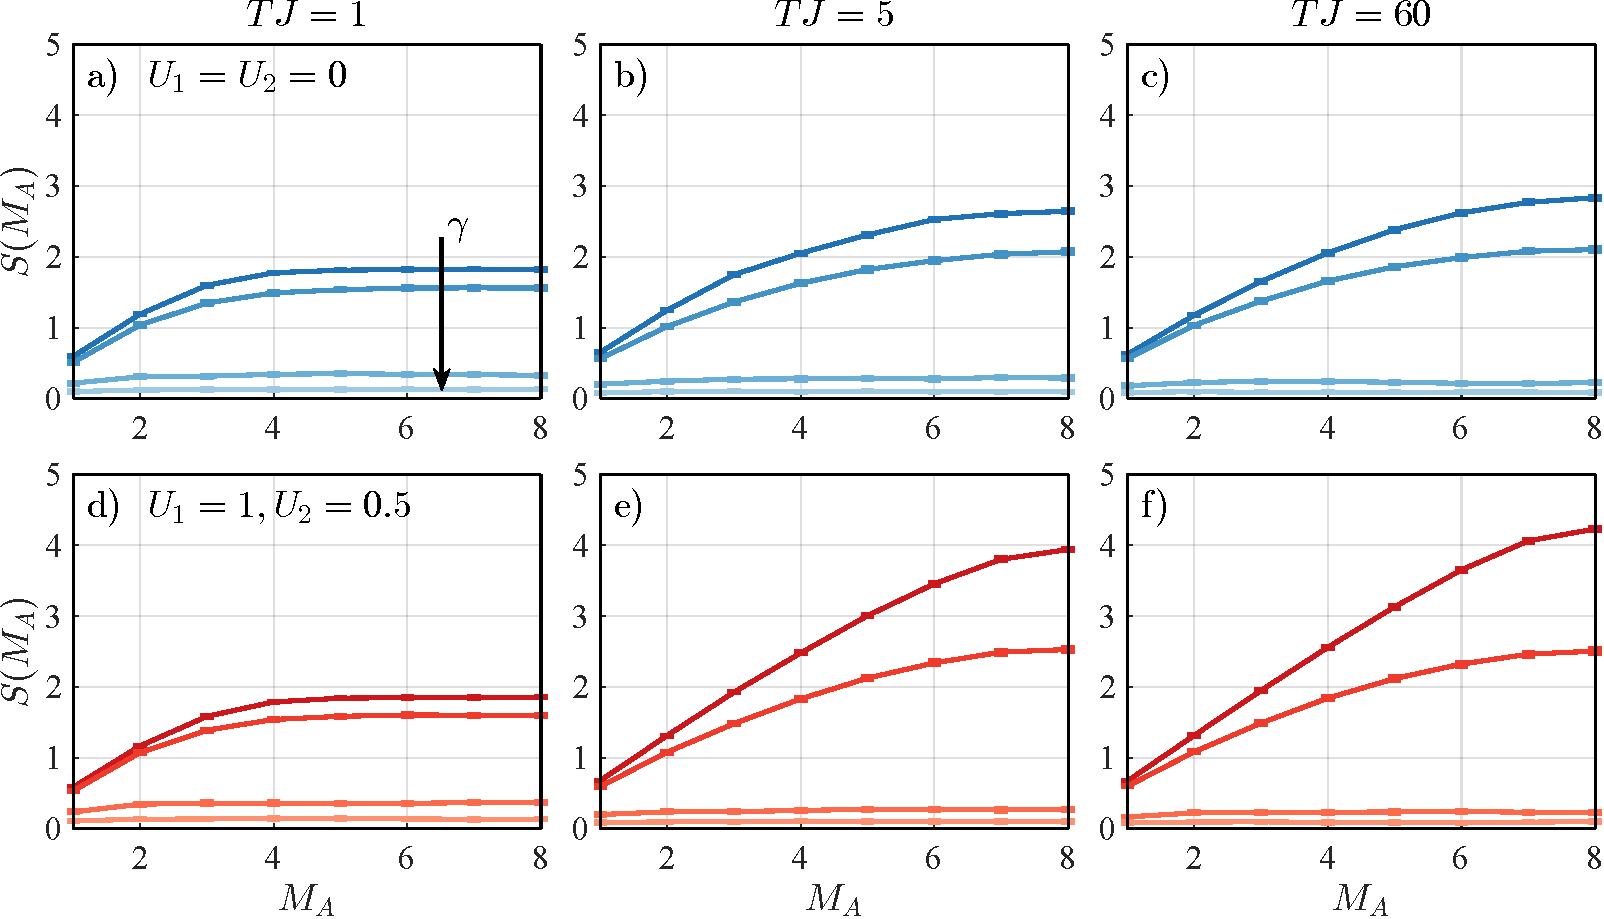
\includegraphics[width=\textwidth]{Chapters/Plots/Chapter6/Chapter5_Fig1.pdf}
    \caption{Snapshots of the von Neumann entropy at three different points in time, $TJ  = [1, 5, 60]$, as a function of subsystem size $M_A$ ($M=16$) for a)-c) the non-interacting model $U_1 = U_2 = 0$, and d)-f) the interacting model with $U_1 = 1, U_2 = 0.5$. We display the entropies for dissipation strengths, $\gamma \in [0.1,0.5,5,10]$, increasing in the direction of the arrow in a). For each snapshot, we time-evolve until $TJ = [1, 5, 60]$, and compute trajectory averages using $N_t = 300$ trajectories.}
    \label{fig:Chapter5_Fig1}
\end{figure}
On the other hand, however, for small measurement rates and at short times, for $TJ = 1$, we see for both the interacting and non-interacting cases in Fig.~\ref{fig:Chapter5_Fig1}a),d) that the entanglement grows with subsystem size to around a subsystem size around $M_A \sim 4$. As only a little time has passed, correlations have not spread further through the system, and hence, at larger subsystem sizes, the entanglement entropy remains constant. At long times for this system size, $TJ = 5$, we now see the entropy behavior in Fig.~\ref{fig:Chapter5_Fig1} b),e) coincides with the steady-state behavior. However, the important conclusion we draw from this analysis is that the qualitative behavior already manifests in the entropy at short times. The quantitative differences arise due to coherent oscillations of the entropy at short times and small measurement strengths. Still, once correlations have been able to travel through the whole system, the qualitative entropy behavior becomes apparent, and we can distinguish the different phases effectively by studying the scaling with time and subsystem size. Note that since we only consider specific snapshots in time, the quantitative entropy behavior changes at intermediate times as a function of the choice of time, which is also a reason why we do not expect to detect the transition itself but rather a crossover region, where features of the transition are already present.

As we have seen, it is possible to clearly distinguish the two regimes, even at early times, where coherent dynamics are still competing with the measurements. Being able to focus on early time dynamics also gives us the advantage of analyzing linear quantities. Starting from a state with all particles initially in odd sites, coherent time evolution allows the particles to hop to neighboring sites and occupy even sites. The coherent time evolution is interrupted by random projective measurements. For small measurement strengths, the unitary time evolution leads to tunneling of the particle to neighboring sites, and projective measurements only rarely occur. In the large measurement regime, measurements occur frequently and project the particles often in odd sites, as they are not able to tunnel to neighboring sites. We further comment on this later in the chapter. To characterize the competition between the coherent dynamics and local projective measurements, we consider the imbalance, defined as the difference between the sum of local densities in event and odd sites,  
\begin{equation}
    \label{eq:imbalance}
    I = (N_e - N_o)/N = \frac{\sum_i (-1)^i \expectation{\hat{n}_i}}{\sum_i  \expectation{\hat{n}_i}},
\end{equation}
where $N_e, N_o$ are the total particle numbers in even and odd sites, respectively, and $N = N_e+N_o$ is the total particle number. For our analysis, we consider an initially imbalanced product state, with all particles in odd sites, and explore how the imbalance relaxes in the presence of measurements. With all particles initially in odd sites, $N_e(t=0) = 0$, and $N_o(t=0) = N$, we have $I(t=0) = -1$. In our model for non-zero measurement rates, at long times, the system loses all information about the initial state, and the average particle number for site $i$ is $\expectation{\hat{n}_i} = 1/2$, hence $I(t\to \infty) = 0$ for all $\gamma \neq 0$. We will now explore the early-time dynamics of the population imbalance and analyze how it relaxes from $-1$ to $0$. 

\begin{figure}[ht]
    \centering
    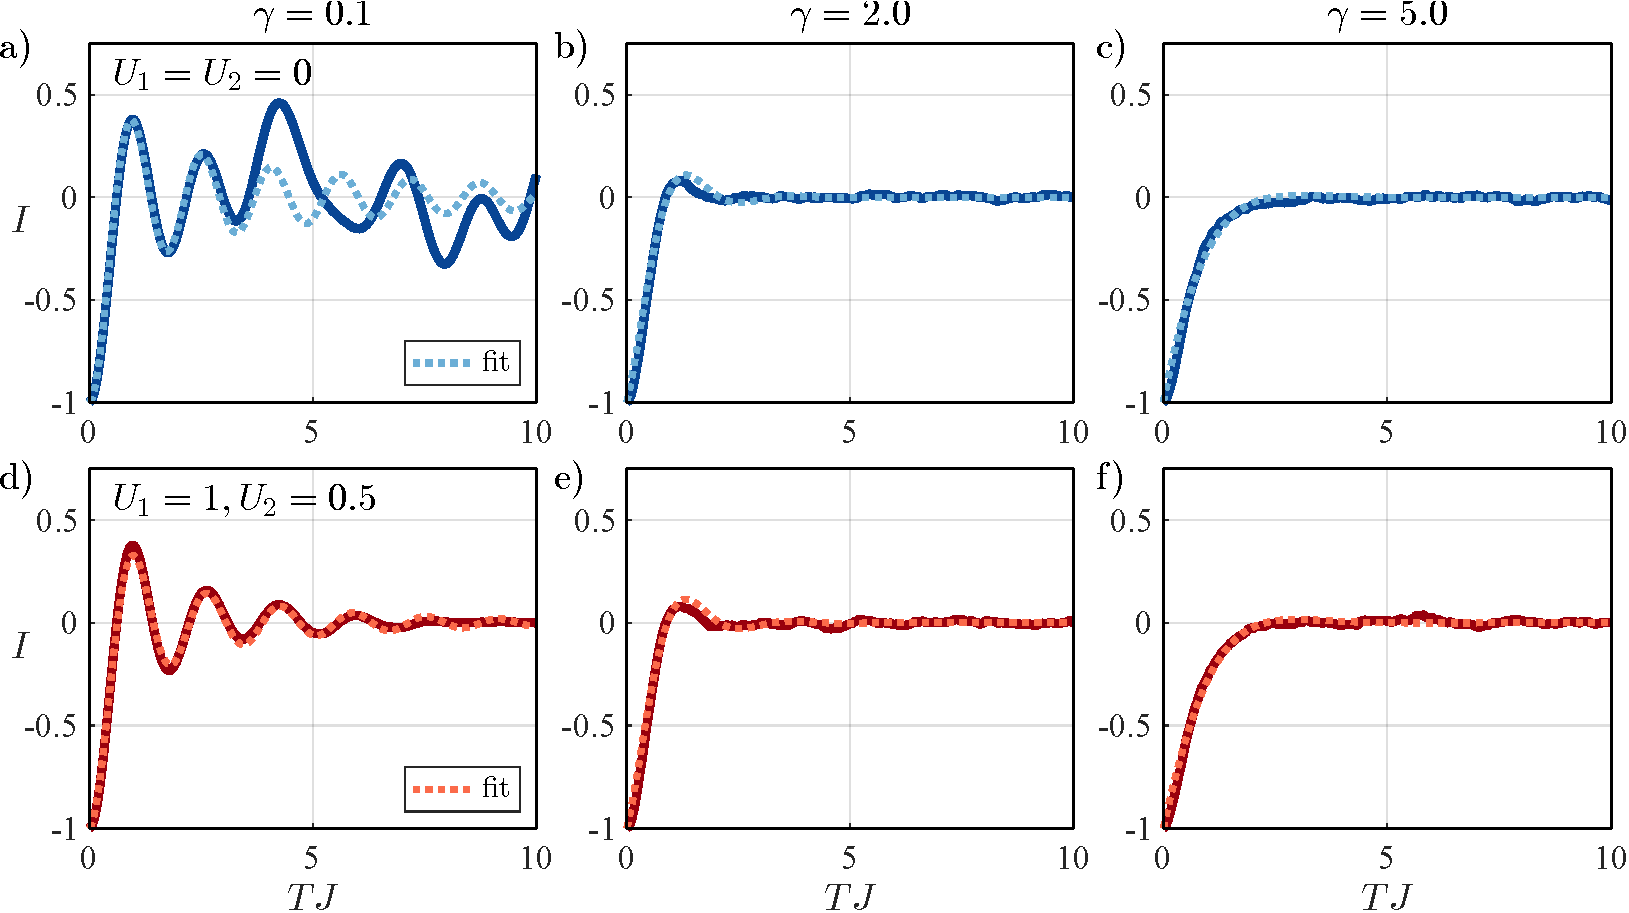
\includegraphics[width=\textwidth]{Chapters/Plots/Chapter6/Chapter5_Fig2.pdf}
    \caption{The population imbalance for a)-c) the non-interacting model $U_1 = U_2 = 0$, and d)-f) the interacting model with $U_1 = 1, U_2 = 0.5$. We display three measurement strengths: a),d) $\gamma=0.1$, b),e) $\gamma=2$, and c),f) $\gamma=5$. For each curve, we also compute a fit of the form $f(t) = J_0(at) e^{-\Gamma t}$, where $J_0$ is the zeroth-order Bessel function of the first kind and fitting parameters $a, \Gamma$. We compute trajectory averages using $N_t = 300$ trajectories.}
    \label{fig:Chapter5_Fig2}
\end{figure}

In Fig.~\ref{fig:Chapter5_Fig2} a),d), we consider the evolution of the imbalance for the measurement strength $\gamma = 0.1$ for the non-interacting and interacting models. In the non-interacting model, finite-size effects are relatively prominent; however, in the interacting model, we can observe dampened coherent oscillations resulting from the competition between the coherent and dissipative dynamics. In the strong measurement regime, depicted in Fig.~\ref{fig:Chapter5_Fig2} c),f), for $\gamma = 5$, the oscillations are fully suppressed as the measurements dominate the dynamics in the system. From our analysis in Chap.\ref{chap:MIPT_bosons} we expect a transition from logarithmic to area-law scaling of the entropy around $\gamma = 2$ and we, therefore, display the imbalance in Fig.~\ref{fig:Chapter5_Fig2} b),e) for this measurement strength. There are no clear visible oscillations for this measurement strength; however, we observe a small increase in the value before the imbalance remains constant around $0$. This analysis clearly shows the competition between the measurements and coherent time evolution, with indications of a transition in the qualitative behavior at around $\gamma = 2$. 

To better understand and analyze the behavior of the imbalance, we also include a fit to the data in Fig.~\ref{fig:Chapter5_Fig2}. In the absence of measurements, the population imbalance in this model follows a zeroth-order Bessel function of the first kind \cite{barmettler2009}. As the coherent oscillations are increasingly stronger damped with growing measurement rate, we characterize the nature of the damping by fitting an exponentially decaying Bessel function to our data of the form, 
\begin{equation}
    f(t) = J_0(at) e^{-\Gamma t},
\end{equation}
where $J_0$ is the zeroth-order Bessel function of the first kind with fitting parameters $a, \Gamma$. In Fig.~\ref{fig:Chapter5_Fig2}, we generally observe good agreement between the fit and the simulated data. In the non-interacting model for small measurement rates, we observe some significant deviations from the fit, which are the result of finite-size effects in the simulation. These deviations, however, are only present for $\gamma < 0.5$ in the non-interacting model, and we otherwise have good agreement with our data and a coefficient of determination $R^2 \approx 1$. 

\begin{figure}[ht]
    \centering
    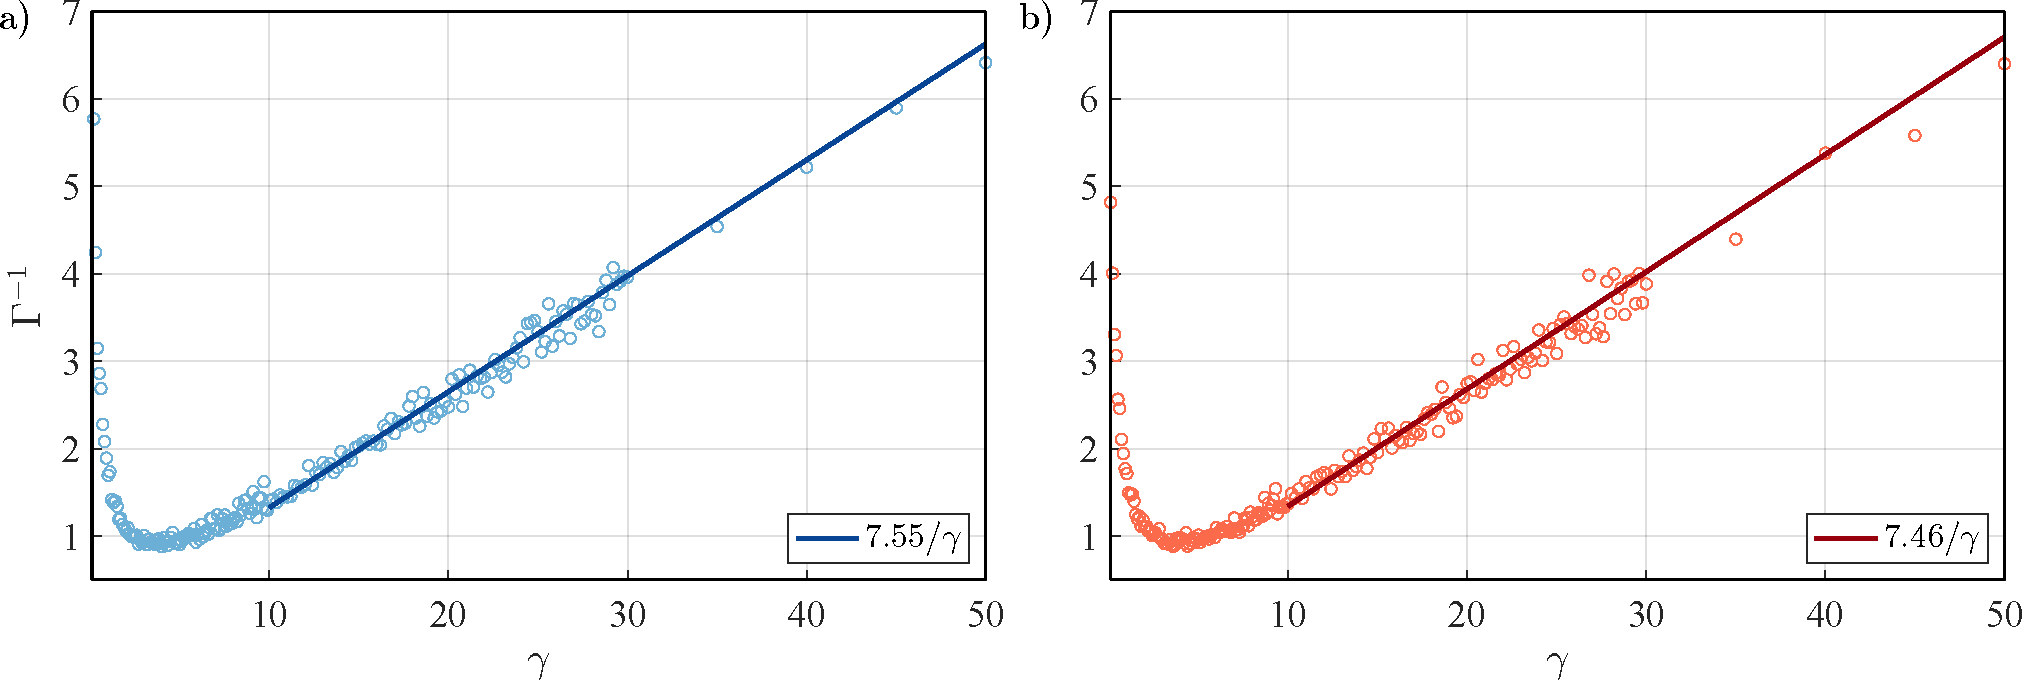
\includegraphics[width=\textwidth]{Chapters/Plots/Chapter6/Chapter5_Fig3.pdf}
    \caption{The fitted damping parameter $\Gamma$ as a function of the measurement strength $\gamma \in [0.1,50]$ for a) the non-interacting model $U_1 = U_2 = 0$, and b) the interacting model with $U_1 = 1, U_2 = 0.5$. The solid lines are fitting functions of the form $f(\gamma) = a/\gamma$ as indicated in the respective legends.}
    \label{fig:Chapter5_Fig3}
\end{figure}

In Fig.~\ref{fig:Chapter5_Fig3}, we analyze the behavior of the damping rate $\Gamma$, and we observe an initial increase of the damping rate $\Gamma$ with increasing measurement strength, indicated by the downward trend of $1/\Gamma$. As the measurements occur more frequently, the coherent oscillations become increasingly suppressed, matching our expectations from the analysis in Fig.~\ref{fig:Chapter5_Fig2}. Once we reach the strong measurement regime, the quantum Zeno effect takes over as particles remain trapped in the initial state for long times and only rarely hop to neighboring sites. Due to this effect, the origin of the suppression of coherent oscillation changes as now the damping rate $\Gamma$ decreases with the measurement strength $\gamma$. 

To better understand the behavior of the damping rate $\Gamma$, let us consider a simple system where only one particle is present in the system at site $j$. The average time between measurements is $1/\gamma$, and after this time, the state has evolved according to 
\begin{equation}
    \ket{\psi(t = 1/\gamma)} = e^{-i H / \gamma} \ket{\psi(t=0)}.
\end{equation}
When $\gamma \gg J$, the system will not have had a lot of time to evolve, and after time $1/\gamma$, the particle will be at site $j$ with amplitude $\sim 1$ or at one of its neighboring sites with amplitude $i J/\gamma$. Then, the measurement projects the particle onto its initial site with probability $\sim 1$ or onto one of its neighboring sites with probability $J^2/\gamma^2$. Therefore, we expect that this process occurs at a rate $J^2 / \gamma$ in the large measurement regime. We confirm that this expectation matches the data as we can observe the linear scaling of the inverse of the damping rate Gamma in Fig.~\ref{fig:Chapter5_Fig3} for large measurement strengths, $\gamma \geq 10$. The scatter points correspond to the simulated data points of the damping parameter $\Gamma$. We then consider a fitting function of the form $f(\gamma) = a/\gamma$, which we fit in the interval $\gamma \in [10, 30]$. We plot the inverse of the fitting function, $f(\gamma)^{-1}$ as a solid line, extending it to the range $[10, 50]$ and see that data points $\gamma > 30$ also follow the trend of the fitted solid line, indicating we have a good fit to the simulated data. 

This analysis suggests that although we are considering a linear function at short times, we can differentiate the area-law regime from the critical regime. Moreover, this analysis seems to fail to find evidence of a volume-law phase in the interacting model for small measurement strengths, which is consistent with the analysis from our previous chapters, where the detection of a volume-law phase has proven to be much more difficult than the transition from the intermediate to the area-law regime. 

\section{Experimental probing of the competition between coherent and dissipative dynamics}

So far, we have seen that non-linear quantities, such as the von Neumann entropy, exhibit signatures in the steady state that allow us to distinguish between the area-law and logarithmic regimes in our model as a function of the measurement strength. Furthermore, experimental detection of the transition using non-linear functions in the density operator is impractical as measurement outcomes are often not reproducible, and techniques for measuring the entropy cannot be used. In the previous section, we have shown that the population imbalance at early times may also be used to detect some features of the transition. In the model we are considering, the population imbalance oscillates due to the competition between coherent time evolution and projective measurements that localize system information. With increasing measurement rates, the oscillations become increasingly suppressed. This allows us to highlight a regime where oscillations become fully suppressed, and the projective measurements dominate the dynamics of the system. Although we cannot study the transition itself using linear quantities at short times, we are able to detect some features that we used to characterize the transition in Chap.~\ref{chap:MIPT_bosons}. 

With this in mind, we will consider a protocol that allows us to probe non-linear correlations at short times in a way that avoids having to access trajectories multiple times. The protocol is based on ideas proposed in Refs.~\cite{elben2018,vermersch2018, vermersch2019}, which allows us to sample the infinite temperature state and extract non-linear information in an experimentally feasible way. We will show that with this protocol, we are able to witness features of the transition by considering the cross-correlations between different measurement trajectories at short times, using random initial states.

\subsection{Protocol}

We begin by preparing an initial product state, $\ket{\psi_0}$, to which we apply local random rotations, 
\begin{equation}
\label{eq:Ru}
    \ket{\psi_0}_u = R_1 \otimes R_2 \otimes ... \otimes R_M \ket{\psi_0} = R_u \ket{\psi_0},
\end{equation}
where $M$ are the lattice sites, and $R_i$ are local random rotations drawn from the circular unitary ensemble (CUE). It can be shown that by averaging over random rotations, we approach the infinite temperature state with increasing precision as we increase the number of random rotations $N_u$ over which we average,
\begin{equation}
    E\big[\ket{\psi_0}\bra{\psi_0}_u\big] = \mathcal{I}/2^M,
\end{equation}
where $E[\cdot]$ denotes the average over many random rotations. This allows us to reliably sample the infinite temperature state and investigate the early-time dynamics using randomly rotated states. 

 In Ref.~\cite{vermersch2019}, the authors develop a protocol to measure out-of-time-ordered correlation (OTOC) functions. OTOCs have been found to be particularly interesting for studying quantum chaos \cite{cotler2018} and quantifying how information travels through many-body quantum systems \cite{hosur2016, chen2016,fan2017,nahum2018a, vonkeyserlingk2018a}. The experimental scheme they propose relies on measuring correlations between local operators, and they prove that it corresponds to the OTOC. In order to measure the cross-correlations between measurement trajectories in our model, we adapt the scheme proposed in Ref.~\cite{vermersch2019}, and we will show that we can use it to highlight features of the transition. 
 
 In particular, the quantity we propose to investigate is the cross-trajectory two-point correlator between local densities,
\begin{equation}
\label{eq:otoc_ru}
    O^{(\hat{n}_i,\hat{n}_j)}(t)= \frac{ E\big[\expectation{\hat{n}_j(t)} \expectation{\hat{n}_i(0) \hat{n}_j(t) \hat{n}_i(0)} \big] }{ E\big[\expectation{\hat{n}_j(t)}^2\big]}.
\end{equation}
where $\hat{n}_i$ is the local number operator acting at site $i$. We now outline the steps in Protocol~\ref{alg:protocol1} required to measure the correlator defined in Eq.~\ref{eq:otoc_ru}.

\begin{figure}[ht]
\begin{algorithm}[H]
\floatname{algorithm}{Protocol}
\caption{Measurement of $O^{(\hat{n}_i,\hat{n}_j)}$}
\label{alg:protocol1}
\renewcommand{\thealgorithm}{}
\begin{algorithmic}[1]
\State Prepare a product initial state $\ket{\psi_0}$ and apply the local random rotation to obtain $\ket{\psi_0}_u = R_u \ket{\psi_0}$, following Eq.~\ref{eq:Ru}. 
\State Apply the operator $\hat{n}_i$ to the randomly rotated state $\ket{\psi_0}_u$. 
\State Time-evolve it using standard quantum trajectory methods to the chosen time $T$ and measure the operator $\hat{n}_j$.
\State Repeat steps 1. and 3. with the same random rotation $R_u$ and measure $\hat{n}_j$ without first applying the local operator in step 2. 
\State Repeat steps 1. - 4. for $N_u$ random rotations and estimate $O^{(\hat{n}_i,\hat{n}_j)}$ using Eq.~\ref{eq:otoc_ru}. 
\end{algorithmic}
\end{algorithm}
\end{figure}

With this protocol, we sample the states from the infinite temperature state, and we can measure $O^{(\hat{n}_i,\hat{n}_j)}$ to investigate the short-time behavior of the system. Another critical factor is that we need to verify that our protocol also works in an experimental setting. To simulate an experimentally detected correlator $\tilde{O}^{(\hat{n}_i,\hat{n}_j)}$, we follow the same steps as in Protocol~\ref{alg:protocol1}, and instead of using the quantum mechanical expectation values, we simulate the experimental expectation values by randomly drawing a $1$ with probability $\expectation{\hat{n}_j(t)}$ and with the default being a $0$. In this way, we can test whether or not our proposed correlator is able to withstand additional noise. 

\subsection{Analysis of the correlator}

Now that we have discussed the protocol, we will look at the short-time dynamics of the correlator in our system. In Fig.~\ref{fig:Chapter5_Fig4}, we plot the correlator $O^{(\hat{n}_i,\hat{n}_j)}(t)$ as a function of time and space, where we chose $\hat{n}_i = \hat{n}_{M/2}$ as local operator to apply at $t=0$. As in our previous analysis, there is almost no qualitative difference between the non-interacting and interacting models, but we observe different behavior based on the measurement strength.

\begin{figure}[ht]
    \centering
    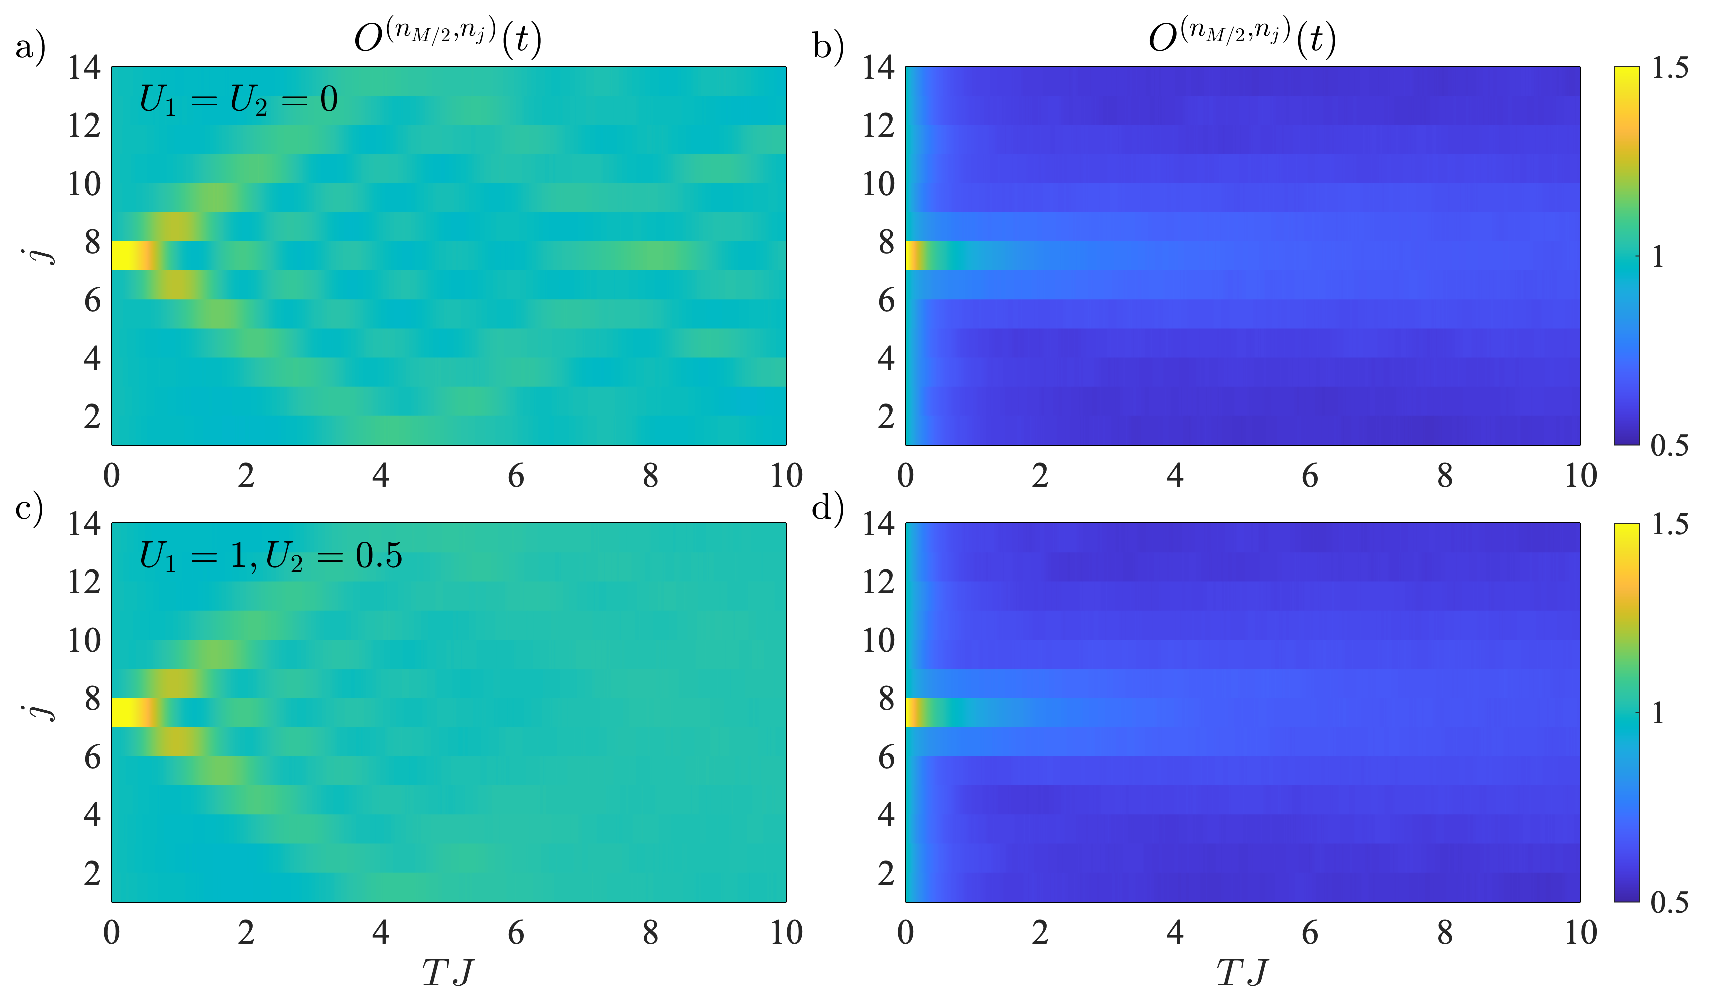
\includegraphics[width=\textwidth]{Chapters/Plots/Chapter6/Chapter5_Fig4.pdf}
    \caption{We plot the correlator $O^{(\hat{n}_{M/2},\hat{n}_j)}(t)$ a), c) for the measurement rates $\gamma = 0.1$ and b), d) $\gamma = 5$ and compare the non-interacting and interacting cases in a), b) $U_1 = U_2 = 0$ and c), d) $U_1 = 1, U_2 = 0.5$. The system consists of $M=14$ sites and time evolve over a range $TJ \in [0, 10]$ using a numerical time step $dt = 10^{-3}$ and average over $N_u = 10^4$ trajectories.}
    \label{fig:Chapter5_Fig4}
\end{figure}

In Fig.~\ref{fig:Chapter5_Fig4}, at $t=0$, the two terms in the numerator differ only at the central site where the operator was applied, highlighting the localized particle. For a small measurement rate $\gamma = 0.1$, we can observe ballistic operator spreading and coherent oscillations traveling through the system. In the interacting model, we additionally see that the oscillations stop after the operator spreading has reached the boundary of the system and the correlator reaches approximately steady behavior around $1$. For a large measurement rate $\gamma = 5$, there appear to be no qualitative differences, and the spreading appears reminiscent of a single particle diffusing in an empty lattice under continuous monitoring. Furthermore, the correlations decay to a value around $0.5$, and the coherent oscillations we saw for the small measurement rate case are fully suppressed by the dissipative dynamics. 

\begin{figure}[ht]
    \centering
    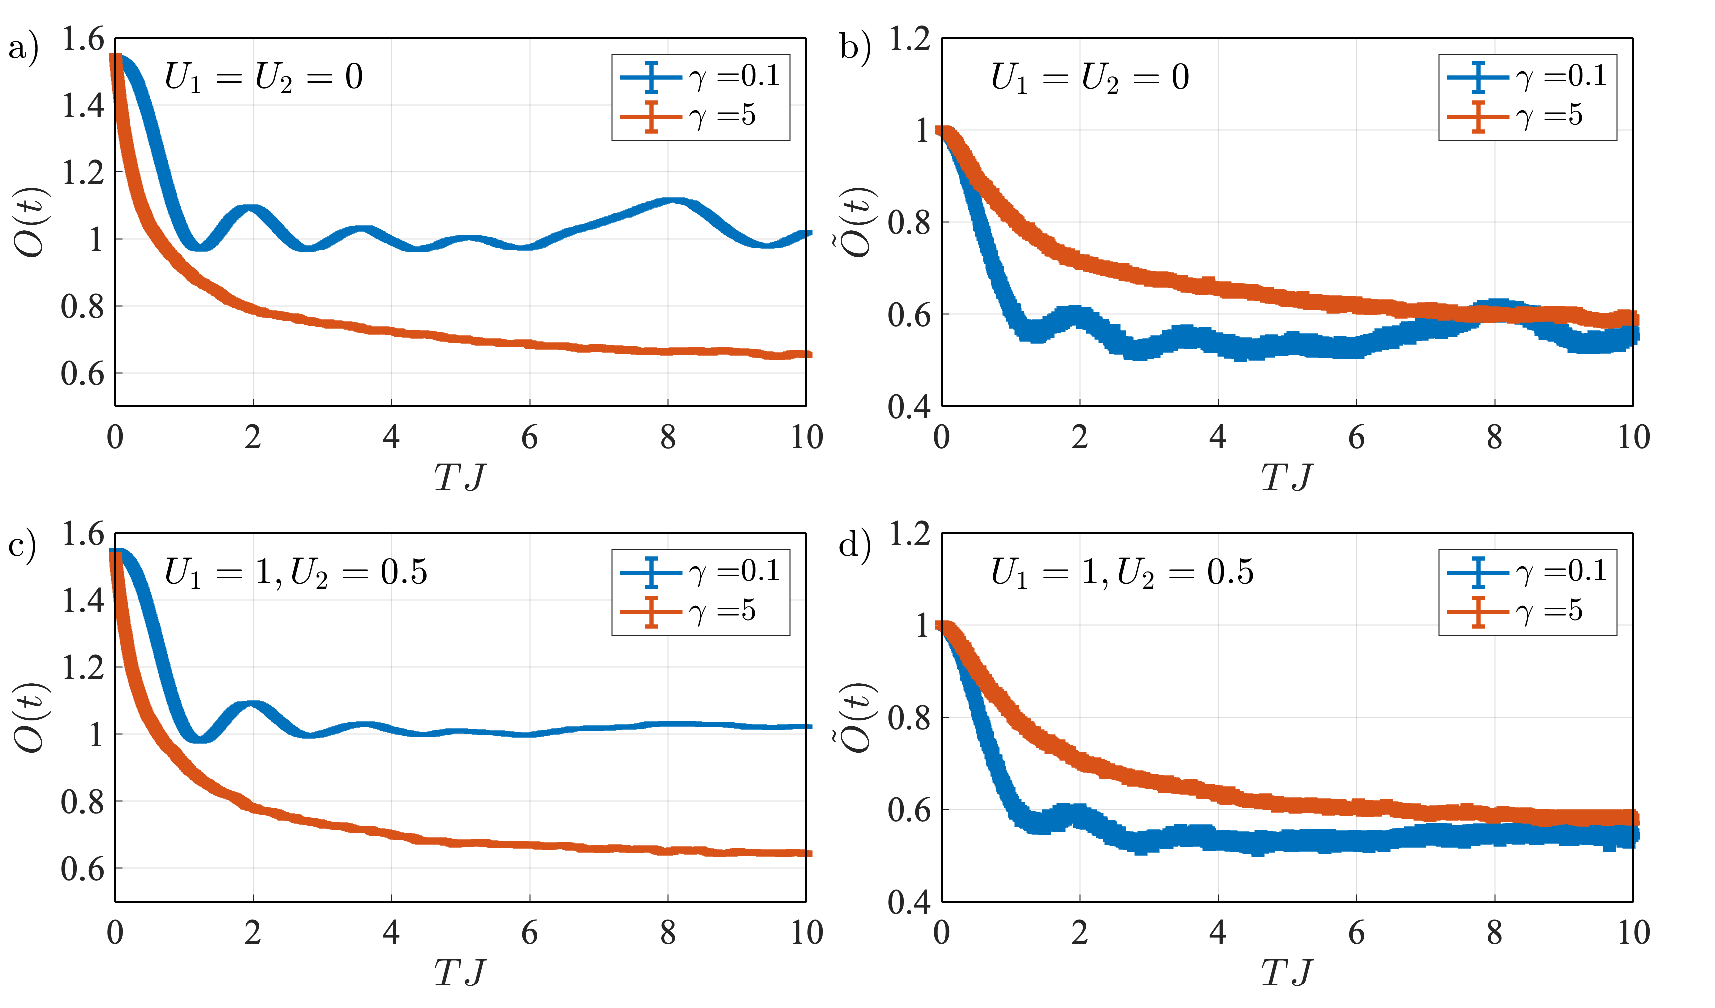
\includegraphics[width=\textwidth]{Chapters/Plots/Chapter6/Chapter5_Fig5.pdf}
    \caption{We plot a), c) the correlators $O^{(\hat{n}_{M/2},\hat{n}_{M/2})}(t) \equiv O(t)$ and b), d) $\tilde{O}^{(\hat{n}_{M/2},\hat{n}_{M/2})(t)} \equiv \tilde{O}(t)$ with $\hat{n}_i = \hat{n}_j = \hat{n}_{M/2}$ as a function of time for varying measurement rates. We compare a), b) the non-interacting, and c), d) the interacting cases. We consider a system of $M=14$ sites and time evolve over a range $t \in [0, 10]$ using a numerical time step $dt = 10^{-3}$ and $N_u = 10^4$ trajectories.}
    \label{fig:Chapter5_Fig5}
\end{figure}

We now more closely analyze the behavior of the correlator at the central site, where we compare $O^{(\hat{n}_i,\hat{n}_j)}$ and $\tilde{O}^{(\hat{n}_i,\hat{n}_j)}$, choosing operators $\hat{n}_i = \hat{n}_j = \hat{n}_{M/2}$. In Fig.~\ref{fig:Chapter5_Fig5}a), c) we plot the correlator in the small and large measurement regimes. The initial behavior for small measurement rates is similar to what we observed for the imbalance; there is an initial drop, and then oscillations appear as we evolve the system in time. In the non-interacting model, in Fig.~\ref{fig:Chapter5_Fig4}~a), we witnessed that once correlations reach the boundary, they travel back towards the center and interact. We also observe this in Fig.~\ref{fig:Chapter5_Fig4}~a), where correlations are damped but around $TJ=5$ increase again and oscillate. In contrast, in the interacting model, this effect is much less prominent, and we observe that around $TJ=5$, the correlator approaches a value $\sim 1$. In the strong measurement regime, however, oscillations due to coherent dynamics are completely washed out, allowing us to distinguish between these two regimes clearly. When we consider the correlator computed from simulated experimental expectation values, in Fig.~\ref{fig:Chapter5_Fig5}b), d), the same qualitative behavior in the two regimes appears. The oscillations in the small measurement regime are weaker due to the additional noise; however, we can still clearly distinguish the dominant coherent behavior in the small measurement regime from the strongly damped behavior in the large measurement regime. 

This analysis shows that we are able to distinguish between the two measurement regimes in both the interacting and non-interacting case, characterized by clear oscillations in the small measurement regime, which are fully damped in the large measurement regime. Since we chose $\hat{n}_i = \hat{n}_j = \hat{n}_{M/2}$, the measurement projects the particle in site $M/2$ at time $t=0$, which means we have, $\expectation{\hat{n}_i(0) \hat{n}_j(0) \hat{n}_i(0)} = 1$ and we obtain,
\begin{equation}
\label{eq:otoc_0}
    O(t=0) = \frac{ E\big[\expectation{\hat{n}_j(0)}\big] }{ E\big[\expectation{\hat{n}_j(0)}^2\big]}.    
\end{equation}
The random rotation of the state leads to a uniform distribution of the expectation values $\expectation{\hat{n}_j(0)} \sim U(0,1)$, with mean $E\big[\expectation{\hat{n}_j(0)}\big] = 1/2$. Given this, we can also find the mean of the distribution of the square $E\big[\expectation{\hat{n}_j(0)}^2\big]$. For simplicity, let us define $\expectation{\hat{n}_j(0)} \equiv N$. First, we need to find the cumulative probability function, 
\begin{equation}
    F_{N^2}(x) = P(N^2 \leq x) = P(0 \leq N \leq \sqrt{x}) = \int_0^{\sqrt{x}} dx = \sqrt{x},
\end{equation}
for $x\in[0,1]$ and using the fact that $N \sim U(0,1)$, where $U(0,1)$ is a uniform distribution on the interval $(0,1)$. To find the cumulative density function $f_{N^2}(x)$, we simply need to compute the derivative of $F_N^2$, 
\begin{equation}
    f_{N^2}(x) = \frac{d}{dx} F_{N^2}(x) = \frac{d}{dx} \sqrt{x} = \frac{1}{2\sqrt{x}},
\end{equation}
for $x\in[0,1]$. Finally, we can compute the mean of the distribution of the squared expectation values,
\begin{equation}
    E\big[\expectation{\hat{n}_j(0)}^2\big] = \int_0^1 x~f_{N^2}(x)~dx = \frac{1}{3}. 
\end{equation}

Substituting both values into Eq.~\ref{eq:otoc_0}, we obtain,
\begin{equation}
    O(t=0) = \frac{1/2}{1/3} = \frac{3}{2},    
\end{equation}
which matches the numerical data in Fig.~\ref{fig:Chapter5_Fig5}.

To compute the expected value at $t=0$ for the experimentally simulated correlator, Eq.~\ref{eq:otoc_0} still holds, however, we need to replace $\expectation{\hat{n}_j}(0)$ with $\expectation{\tilde{n}_j}(0)$, where $\tilde{\cdot}$ denotes that we replace the quantum mechanical expectation value with a $1$ with probability $\expectation{\hat{n}_j}(0)$ and a $0$ otherwise. Given a large enough sample size, when we compute the mean, it remains $1/2$. Since all values are either $0$ or $1$, however, this implies that the distribution of the squares remains unchanged and the mean of $\expectation{\tilde{n}_j}(0) = 1/2$.

Hence, we obtain, 
\begin{equation}
    \tilde{O}(t=0) = \frac{1/2}{1/2} = 1, 
\end{equation}
which also matches our numerical data. Interestingly, the dynamics of the correlator $O(t)$ are still captured by the simulated correlator $\tilde{O}(t)$, giving us an experimentally feasible protocol to show the behavioral difference of this quantity in the two regimes. 

This protocol, however, does have some drawbacks; namely, firstly, for the numerical simulation, we need a very small numerical time step, making it slower and, secondly, a large number of trajectories is needed to reduce the statistical noise enough to distinguish the signals in the two regimes. Since we are sampling the infinite temperature state, we need approximately $N_u \propto 2^M$ trajectories in order to get an accurate experimental signal. Due to these limitations, it becomes difficult to simulate larger systems as well as detect these quantities experimentally when the number of trajectories grows exponentially with the system size.

\section{Conclusion}

In this chapter, we further analyzed the competition between coherent and dissipative dynamics in a bosonic system, with and without interactions, by probing the small and large measurement regimes using linear and nonlinear functions in the density operator at short times. In chapter~\ref{chap:MIPT_bosons}, we showed the MIPT can be visualized using non-linear quantities, such as the von Neumann entropy at long times, and we can clearly distinguish between volume-law and area-law entanglement phases. The experimental detection of the MIPT proved to be a difficult obstacle, as measuring non-linear quantities requires accessing individual trajectories multiple times. Quantities that are linear in the density operator are not able to distinguish between the phases as the steady state is the featureless infinite temperature state. The main idea of this chapter was to relax these constraints of needing non-linear quantities at long times and instead analyze linear quantities at short times to find out whether or not this still allows us to distinguish features associated with the two phases, even if we cannot access the transition itself at short times. We first considered the von Neumann entropy to investigate whether the phase transition would still be present at short times, and we saw that for large measurement strengths, the entropy barely increases and already at very short times ($TJ \sim 1$) has reached its steady-state value. For small measurement strengths, however, the entropy still changes considerably at short times. However, its qualitative behavior is already clearly visible in small subsets of the whole system. This is due to the fact that correlations have not yet traveled through the system, but as the measurements occur infrequently in this regime, coherent dynamics dominate the behavior of the system. We next analyzed what happens to the population imbalance, which is defined as the difference between the population at odd and even sites normalized to the total particle number. This quantity is linear in the density operator and will approach $0$ as the local densities approach $1/2$ at long times for any non-zero measurement strength. In a system not subjected to measurements, the imbalance is described by a zeroth-order Bessel function. By introducing measurements, we saw that the coherent oscillations are increasingly suppressed with increasing measurement strengths. By fitting an exponentially decaying Bessel function, we were able to show that first, the strength of the damping increases with increasing measurement strength. After some point, due to the quantum Zeno effect, the damping rate decreases again, but oscillations continue to be increasingly suppressed as the particles remain trapped in the initial state for long times. It is interesting that this change occurs in the same regime where we expect the phase transition, and this analysis allows us to highlight this behavioral change. Finally, in this chapter, we analyzed a correlator that is non-linear in the density operator and proposed a protocol that allows us to measure it without needing to access individual trajectories multiple times. We achieve this by sampling from the infinite temperature by sampling random rotations of the initial state and analyzing the short-time behavior of the correlator. Although the protocol is numerically expensive to simulate, it has allowed us to demonstrate that we are able to distinguish between the two phases by showing that in an experimental setting, we can observe coherent oscillations for small measurement strengths, which are fully suppressed in the large measurement regime, leading to results closely related to what we saw from the analysis of the population imbalance. Experimentally, to implement this protocol, single-site control is required to prepare the initial states and apply the random rotations. Moreover, single-site resolution of the local particle number is required to evaluate the correlator we have proposed. Current experiments in quantum gas microscopes \cite{bakr2009, blatt2012, gross2017, gross2021} are promising examples where the local dissipation can be realized through noise or light scattering \cite{pichler2010, luschen2017, poletti2013, sarkar2014}. 
	
	\chapter{Conclusion}
\thispagestyle{empty}
\label{chap:conclusion}

In this thesis, we have explored measurement-induced phase transitions in continuous time models that result from the competition between coherent and dissipative dynamics. These transitions manifest in non-linear steady-state properties in many-particle quantum systems accessible only at the trajectory level since the system approaches the structureless infinite temperature state at long times, independent of the measurement or dissipation strength. To experimentally measure non-linear quantities, one would require accessing individual trajectories multiple times, making it challenging to find suitable quantities that reveal the phase transition in an experiment. We now summarize the ways in which we explored ways to understand these transitions better and find a way to detect them experimentally. 

In chapter~\ref{chap:MIPT_bosons}, we presented the measurement-induced phase transition that arises from the interplay between coherent time evolution and dissipative dynamics in a bosonic $1$D chain. The von Neumann entropy best characterizes the transition; for small dissipation strengths, we observed a volume-law phase where the entropy increases linearly with subsystem size, while for large dissipation strengths, we observed an area-law phase, where the entropy is approximately constant. At intermediate dissipation strengths, the entropy scales approximately logarithmically. To pinpoint the exact location of the transition, we performed a scaling collapse analysis of our numerically simulated data and concluded that we could not pinpoint the transition accurately. This was largely due to the fact that we were not able to simulate large enough system sizes, which in random circuit models, where such transitions were studied first, is not a problem as the numerical tools allow simulation of much larger system sizes. We considered two dissipative processes: dephasing and single-particle gain or loss. We showed that the exact type of dissipation did not make a difference. The $U(1)$ symmetry is broken for single particle loss or gain; however, the outcome of the scaling collapse analysis did not change. 

Then, in chapter~\ref{chap:MIPT_continuous_measurement} we shifted our focus to experimentally detecting the phase transition we studied in chapter~\ref{chap:MIPT_bosons}. We considered free fermions in a $1$D chain subject to weak measurements, which can be simulated for larger system sizes under the evolution of a quadratic Hamiltonian. The method for experimental detection we proposed was based on first rewriting a non-linear correlation function in the density operator as a function of local number operators. The transition is characterized by this correlation function, which decays algebraically in the small measurement regime and exponentially in the large measurement regime. Secondly, in the context of weak measurements, the natural choice was to consider a homodyne detection setup, where the measured output signals are homodyne currents, which contain only linear information in the density operator. In our case, this means that by averaging many homodyne currents, we can measure the local densities and use this to reconstruct the correlation function that characterizes the transition. However, we proved that extracting the correlation function using only homodyne currents is impossible, as the non-linear cross-product terms cancel out when computing the averages, rendering the protocol not feasible for experimental detection.

Finally, in chapter~\ref{chap:short_time_dynamics}, we asked whether detecting the competition between coherent and dissipative dynamics at early times during the system evolution is possible, considering the same model as in chapter\ref{chap:MIPT_bosons}. First, we showed that the von Neumann entropy at short times displays characteristic behavior associated with the phase transition. Secondly, coherent and dissipative dynamics are competing at short times, and we used a linear function, namely the population imbalance, to analyze the early time dynamics. We fitted an exponentially decaying Bessel function to the simulated data and analyzed the fitting parameters. We observed that the damping rate increases to approximately the dissipation strength at which we expect the transition to occur and then decreases algebraically. Lastly, we proposed a protocol in which randomly rotated states are sampled from the infinite temperature state, as they provide a way to reproduce initial states reliably. By measuring the number operator in a specific way, we showed that we could construct a correlation function that is able to display similar characteristic behavior we saw in the analysis of the population imbalance, therefore providing an experimentally feasible method to visualize features of the transition even if we cannot probe the transition itself. 

To summarize, we have analyzed a range of continuous time models in which measurement-induced phase transitions appear and explored some ways in which the competition between coherent and dissipative dynamics can be observed experimentally. Although these transitions can be studied using standard numerical methods to simulate the models, finding an experimentally feasible protocol is difficult, as we showed in this thesis. The main difficulty comes from the fact that the transition is masked at the level of the density operator and the restriction of being unable to access individual trajectories multiple times. 
		
    \printbibliography
	
\end{document}
